% !TEX TS-program = pdflatex
% !TeX encoding = UTF-8

\documentclass[a4paper,%
						11pt,%
						twoside,%
						english,%
						evenboxes,%
						numerazioneromana]{toptesi}
\usepackage[utf8]{inputenc}
\usepackage[T1]{fontenc}
\usepackage{lmodern}
\usepackage[a-1b]{pdfx}
\usepackage{hyperref}
\usepackage{cite}
\usepackage{listings}
\usepackage{color}
\usepackage{url}
\usepackage{multirow}
\usepackage{amsmath}
\usepackage{amsfonts}
\usepackage{amssymb}
\usepackage{amsthm}
\usepackage{subcaption}
\usepackage{xpatch}
\usepackage{cancel}
\usepackage{tcolorbox}

\ifpdf
\graphicspath{{Figures/}{Figures/PDF/}{Figures/}}
\else
\graphicspath{{Figures/Vector/}{Figures/}}
\fi

\lstdefinelanguage{P4}
{
	% list of keywords
	alsoletter=\#,
	morekeywords={
		header\_type,
		fields,
		header,
		parser,
		extract,
		return,
		default,
		next,
		\#define,
		latest,
		select,
		apply,
		control,
		table,
		reads,
		actions,
		modify\_field,
		action,
		valid,
		nop,
		exact,
		lpm,
		if,
		hit,
		and,
		extern,
		void,
		bit
	},
	sensitive=true, % keywords are not case-sensitive
	morecomment=[l]{//}, % l is for line comment
	morecomment=[s]{/*}{*/}, % s is for start and end delimiter
	morestring=[b]" % defines that strings are enclosed in double quotes
}

\definecolor{eclipseBlue}{RGB}{42,0.0,255}
\definecolor{eclipseGreen}{RGB}{63,127,95}
\definecolor{eclipsePurple}{RGB}{127,0,85}

\lstset{
	language={P4},
	basicstyle=\fontsize{8}{9}\ttfamily, % Global Code Style
	captionpos=b, % Position of the Caption (t for top, b for bottom)
	extendedchars=true, % Allows 256 instead of 128 ASCII characters
	tabsize=2, % number of spaces indented when discovering a tab 
	columns=fixed, % make all characters equal width
	keepspaces=true, % does not ignore spaces to fit width, convert tabs to spaces
	showstringspaces=false, % lets spaces in strings appear as real spaces
	breaklines=true, % wrap lines if they don't fit
	frame=trbl, % draw a frame at the top, right, left and bottom of the listing
	%frameround=tttt, % make the frame round at all four corners
	framesep=4pt, % quarter circle size of the round corners
	numbers=left, % show line numbers at the left
	numberstyle=\tiny\ttfamily, % style of the line numbers
	commentstyle=\color{eclipseGreen}, % style of comments
	keywordstyle=\color{eclipsePurple}, % style of keywords
	stringstyle=\color{eclipseBlue}, % style of strings
}

\hypersetup{%
    pdfpagemode={UseOutlines},
    bookmarksopen,
    pdfstartview={FitH},
    colorlinks,
    linkcolor={blue},
    citecolor={blue},
    urlcolor={blue}
  }

\newtheorem{osservazione}{Osservazione}% Standard LaTeX
\newtheorem{definition}{Definition}

% patch proof command for bold-face fond
\xpatchcmd{\proof}{\itshape}{\normalfont\proofnamefont}{}{}
\newcommand{\proofnamefont}{}
\renewcommand{\proofnamefont}{\bfseries}

\mathchardef\mslash="202F
\DeclareMathOperator*{\dprime}{\prime \prime}

\begin{document}
%\blankpagestyle{empty} %no numbers in blank pages
\english
\ateneo{Politecnico di Torino}
\corsodilaurea{Communications and Computer Networks Engineering}

\titolo{Optimized Flow Scheduling for Low Latency Data Center Networks}

\candidato{Alessandro \textsc{Cornacchia}}
\relatore{Prof.\ Paolo \textsc{Giaccone}}
\secondorelatore{Prof.\ Andrea \textsc{Bianco}}
\sedutadilaurea{\textsc{Academic~Year} 2019-2020}
\logosede{Frontespizio/Logoblu}

\CorsoDiLaureaIn{Master Degree course in\space}
\TesiDiLaurea{Master Degree Thesis}
\InName{in}
\CandidateName{Candidate}
\AdvisorName{Supervisors}
\sedutadilaurea{July 2020}
%\Materia{Ciao micia}
\frontespizio

\paginavuota

%\begin{dedica}
%	"Credo che la curiosità sia l'unica cosa di cui abbiamo bisogno nella vita. Se sei curioso troverai la tua passione e i risultati che avrai saranno il frutto di quanta passione metterai nella tua vita".
%\end{dedica}

\ringraziamenti

Thanks

\abstract
Major cloud computing providers agree on denoting the Flow Completion Time (FCT) as one of the primary goals to achieve in the design of a Data Center Network (DCN). This is motivated by the fact that latency affects the performance of interactive cloud computer services, such as web search, social networks and online applications, with a direct impact on the Quality of Experience as perceived by end users, hence ultimately on provider revenues.

Several approaches in literature rely on priority mechanisms at flow or packet level and schedulers in the network to reduce the average and tail FCT of latency-constrained flows. 
% albeit for many applications also tail latency is important. 
To this purpose, the Shortest Remaining Processing Time (SRPT) scheduling policy is proven to be optimal when the job size is known in advance. Unfortunately, this information is rarely available and would require expensive modifications to the protocol stack. Therefore, some proposals emulate a size-agnostic scheme that gives precedence to the flow with Least Attained Service (LAS), exploiting a finite number of priority queues in network switches. The effectiveness of these algorithms largely depends on the number of priority levels employed. However, DCNs are usually realized with low cost commodity devices, where only few queues per port - typically two - are vacant.

The contribution of this work is to investigate a design which exploits path abundance --- offered by DCN Fat-Tree topologies --- to intelligently route flows across the switching fabric, depending on their priority. The basic idea is to consider multiple switches as a whole switch, sharing the priority queues. Flows are scheduled both across priority queues and across multiple links, thus augmenting the priority granularity with spatial diversity. 
%In this load balancing and prioritization are jointly analyzed, in what multiple links together provide higher priority granularity than a port alone. ... with a scope limited to single bottleneck interfaces, the problem can be 
In short, flow scheduling is addressed at DC-wide level, considering the queues of different equal cost links together. Hence, unlike aforementioned techniques, load balancing and prioritization are jointly analyzed, since load balancing directly depend on flow priorities. This approach seems appealing for its very limited complexity. 

First, an analytical model is provided for the setting of optimal parameters. Then, it will be shown through a numerical fluid-model simulator that the proposed strategy indeed is helpful when the flow serving policy is FIFO. Conversely, few unexpected impairments under Processor Sharing discipline have been discovered. They are deeply analyzed, in relationship to the size of the topology and to the number of priority queues per interface. Finally, a broad spectrum of packet level simulations in a real data center topology have been conducted with OMNeT++ discrete-event simulator, in order to validate the FCT trends obtained in previous steps. 
%, but that long flows can be excessively penalized. .....
%We were able to show the same FCT trends and provide few additional insights . At the same time, we were able to identify downsides of this methodology and provide a possible strategy to overcome them.

%\tablespagetrue
\figurespagetrue
\indici

\mainmatter
\chapter*{Introduction}
\addcontentsline{toc}{chapter}{Introduction}
In the last decades,  with the spreading of cloud services accessible to anyone, computing has undergone a remarkable evolution. Encouraged by the astonishing growth of virtualization technologies in the IT industry, as well as the availability of storage and chips at ever-more modicum prices, over-the-top (OTT) players like Google, Amazon and Microsoft, have been building datacenter hotspots all around the world. Their data center infrastructures house critical applications for most business activities, such as commercial and financial services, Web search, scientific computing, on-demand video streaming, recommendation systems, not to mention social networking and online gaming. Indeed, from small enterprises to large corporations it has been a common cost-saving strategy to offload, up to a certain extent, the deployment and operation of their own information systems to third parties, the cloud service providers. Computing resources have been being centralized in data centers facilities and shared among plenty of customers, enabling better resource utilization. \\
At the same time, cloud computing posed notable issues in the design, scalability and mantainance of systems running the aforementioned services. A major challenge is certainly the design of a huge capacity communication network hosting hundreds of thousands of servers, while guaranteeing
% that is required to simultaneously provide high throughput and low-latency, 
uninterruptible service continuity and relentless expansion. Unlike traditional TCP/IP networks such as the Internet, the data center network is characterized by a massive amount of equipment confined in a circumscribed area and administrated by a single entity, able to embrace changes to legacy protocol stack in order to accommodate their needs. 
Vast scientific literature has been produced by the research community, addressing new solutions for efficient network operations in the data center. Its peculiar environment have pushed the deployment % exploration the lack of flexibility of 
of unconventional approaches, such as centralized control and network softwarization (SDN/NFV), laying the premises for a wide transformation process in the network industry. In this sense, datacenters can be credited to having represented natural incubators for part of the evolution of telecommunication networks happening during the last few years. As a matter of fact, virtualization technologies and control plane programmability would have become soon disruptive innovations in the networking ecosystem.
%, that started to experience the same changes the IT world faced years before.
%Pushed by datacenters' needs, the research community, both from industry and academia, started to work on innovative solutions that ...  
As a result of this process, nowadays, Internet Service Providers are trying to convert their infrastructure towards the same solutions, re-architecting PoPs as small-scale datacenter, with massive employment of virtualization as regards network functions and devices. Similarly, the next generation mobile network, 5G, is going to base both its core and edge functions on the same paradigm, as revealed by its standardization and by the investments in Multi-access Edge Computing. 

In a Data Center Network (DCN) coexist traffic of a myriad applications and generally belonging to different tenants, which may have contracted a Service Level Agreement (SLA) with the provider. In general, flows with different Quality of Service (QoS) demands share the same resources. Some applications require low latency in delivering their data across servers, whereas others only require huge bandwidth but are less sensitive to timing constraints. Delays on flows that are generated by interactive applications --- like web search or social networks --- have a direct impact on the quality of user experience. Indeed, the responsiveness of these services is crucial to gain user satisfaction, hold customers in the long term and ultimately to determine revenues. As a consequence, all data center providers seek for traffic control algorithms that accomplish low response times for this kind of flow, while ensuring maximum resource utilization in the network and QoS guarantees for coexisting flows. Many of these solutions rely on advanced transport protocols and schedulers in the network to handle different flows with different priorities. The goal of this research is to devise a traffic control scheme that improves the performances of state-of-the-art schedulers, without introducing additional complexity. As it will be extensively discussed hereafter, the proposed algorithm aims to exploit one property of modern data center topologies to enhance the capabilities of current scheduling strategies. 

The remainder of this work is organized as follows. Chapter \ref{ch1} is a review of the design and management principles of data center networks. It describes reference architectures for modern interconnection fabrics, adopted in practice by main players such as Google and Facebook. Then, it reports the main characteristics of data center traffic, measured in production scenarios. Finally, it exposes in details the goals of traffic control schemes and illustrates the failure of legacy protocols, like the TCP, in meeting applications requirements. Next, Chapter \ref{ch:theoretical-scheduling-bg} focuses on scheduling disciplines that best perform with data center's traffic properties in minimizing the Flow Completion Time (FCT). Some theoretical background is provided, together with two practical proposals that leverage switches priority queues (PQ) to target ideal performances. Then, Chapter \ref{ch:sdframework} presents the key idea of the present work, referred to as \emph{spatial diversity}. In the first part it is illustrated qualitatively how it works and why it should give benefits. In the second part, it is formulated an analytical model that will be used for setting the parameters involved in the system and adopted in its evaluation in subsequent chapters. Specifically, the validation of the system traversed two stages. Chapter \ref{ch:numerical-simulator} describes a set of results obtained through a numerical job-level simulator, which neglects all the aspects of a real data center network implementation, rather it simulates flows as jobs in an equivalent queuing model. The outcomes of this step have been of uttermost importance for understanding the advantages and the limitations of the proposed approach. Finally, its implementation in a data center network is shown in Chapter \ref{ch:dcn-simulations}, confirming similar trends to the numerical model. A broad spectrum of simulations have been carried out with the academic and educational license of the OMNeT++ framework and the INET library. Computational resources have been kindly provided by the High-Performance Computing facility of Politecnico di Torino and required engineering few MPI routines for best appreciating parallelism gains. Also, a working implementation of Data Center TCP (DCTCP) --- currently not available for the network simulator tool ---  has been delivered and it will be shared with the interested community under open source license.
%Since web applications pay also extra delays when traversing the Internet to reach the end-user, latencies inside the data center must be within tight constraints, on the order of some milliseconds. A design principle driving the development of the system is its ease of deployment with current technologies without expensive hardware/software modifications.
\chapter{Datacenter networks}
\label{ch1}
% pervasive extensively widespread make use of massively plenty 
%\section{Datacenter design and management principles}
% dire che è semplice perchè unica entità amministrativa e single location
\section{Interconnection network design}
\label{sec:topology}
The typical structure of a datacenter, as shown in Fig.\ref{fig:topology},  
is comprised of many \textit{racks}, interconnected among each other thanks to a common network infrastructure. A rack is nothing else than a group of servers physically co-located in a common cabinet, attached to the same \textit{Top of Rack} switch (ToR) and thus  separated by a single hop. In achieving the goal of hosting an enormous amount of servers, the principal bottleneck often results in being the interconnection fabric, usually referred to as \textit{Data Center Network} (DCN). Ideally, it should act as a huge switch, able to provide maximum-rate communication among servers, that is their NIC's access capacity.  At high level, there are fundamentally two ways for practically realizing such infrastructure. The first choice is to rely on complex specialized solutions, like InfiniBand, or high-performance IP devices with many ports, that successfully provide bandwidth for thousands of nodes, however incurring in high deployment and management costs. Conversely, the second possibility is to build the network infrastructure by simply leveraging on commodity off-the-shelf switches that are cheaper, already on economy of scale and fully compatible with existing hardware and operating systems, just as large distributed clusters are made of general purpose cheap computers. This is usually the design pursued by principal cloud providers, as recently disclosed by some of them \cite{jupiter, facebook_dcn}. A major drawback of the latter strategy, is the difficulty in providing full-rate communication among hosts in different racks. In other words, depending on traffic patterns and especially network topology, it is very hard to place enough inter-rack capacity - usually referred to as \textit{bisection bandwidth} - to satisfy the collective demand of all the racks. 
For this reason, the topology design plays a fundamental role for the feasibility of scalable and cost-beneficial large datacenters. It is worth noticing that sometimes, building a DCN with full bisection bandwidth is unnecessary and cost prohibitive, therefore it is commonly accepted some degree of \textit{oversubscription}, meaning that the ratio between total intra-rack and bisection bandwidth is greater than 1. This choice is acceptable when applications are mostly rack local and statistical multiplexing is beneficial. In general, a non-oversubscribed network allows greater flexibility in resource allocation and deployment of applications across racks, leading to higher utilization which is also important for big cloud providers.
\begin{figure}
	\centering
	\begin{subfigure}[b]{0.45\textwidth}
		\centering
		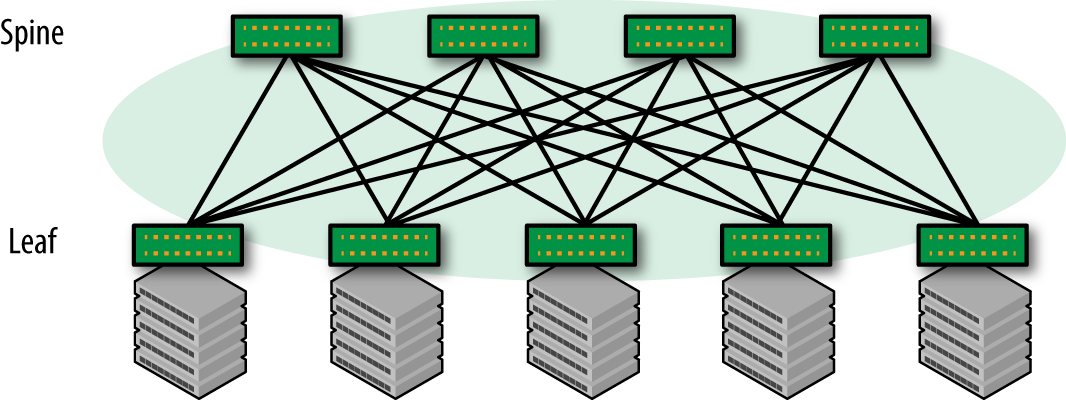
\includegraphics[width=\textwidth]{Chapter1/Figures/leaf-spine}
		\caption{Leaf-Spine}
		\label{fig:leafspine}
	\end{subfigure}
	\hfill
	\begin{subfigure}[b]{0.45\textwidth}
		\centering
		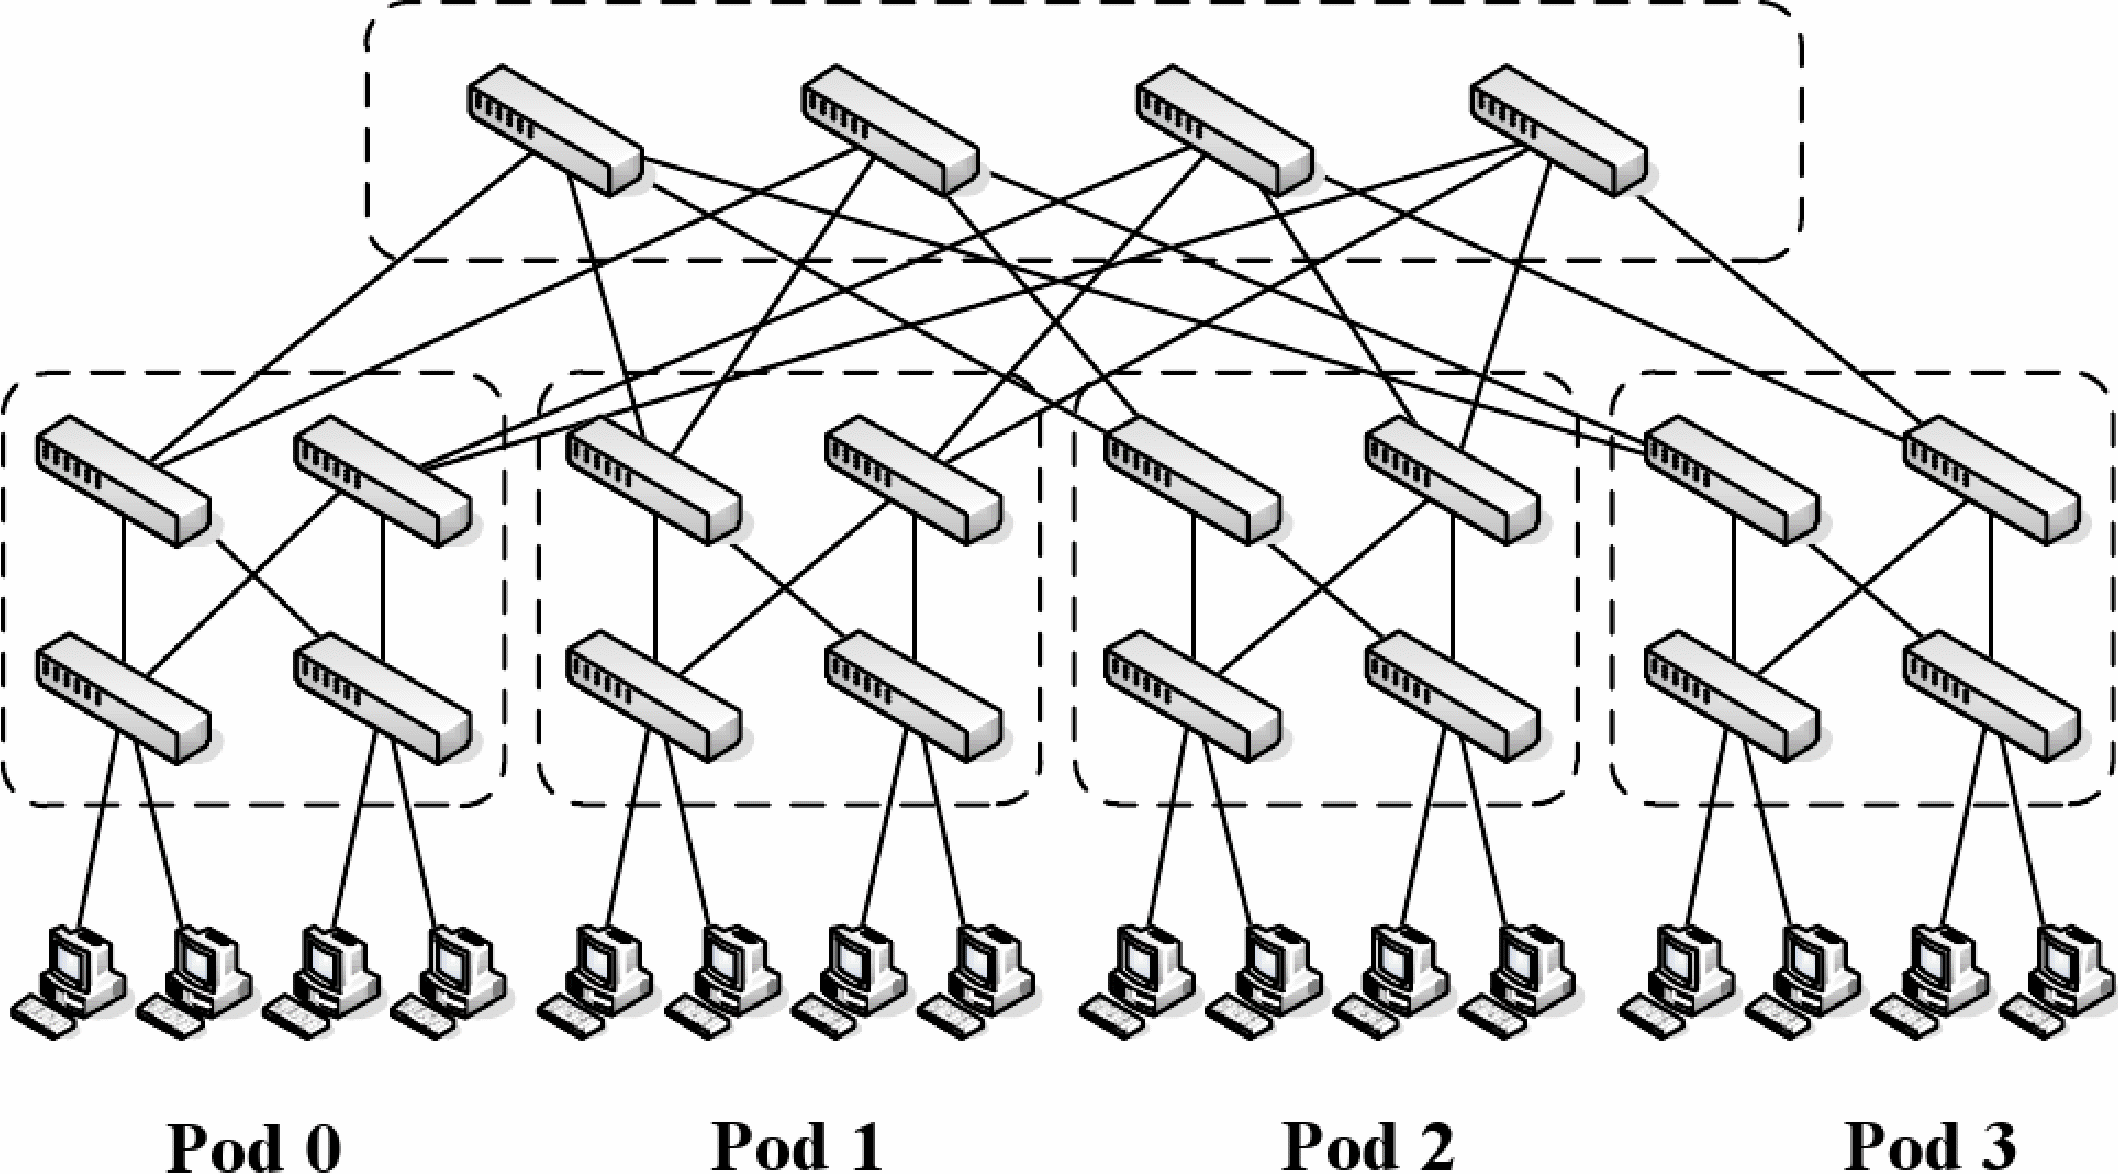
\includegraphics[width=\textwidth]{Chapter1/Figures/fat-tree}
		\caption{3-layers Fat-Tree}
		\label{fig:fattree}
	\end{subfigure}
	\caption{interconnection networks.}
	\label{fig:topology}
\end{figure}

Two examples of topology design are provided in Fig. \ref{fig:topology}.
The \textit{Leaf-Spine} (Fig. \ref{fig:leafspine}), is a typical hierarchical architecture, where the interconnection between leaf and spines switches form a bipartite graph. Despite being popular in campus networks, scaling to thousands of servers would require having spines with lots of high-capacity ports .  
%In general, the desired properties can be summarized in:
%\begin{itemize}
%	
%	\item \textbf{Non-blocking}
%	
%	\item \textbf{Scalable}
%	
%	\item \textbf{Fault tolerant}
%	
%\end{itemize}
A more flexible solution dates back to the early telephone network, when Charles Clos had to solve a similar problem and came up with its proposal for multi-stage switching fabrics. Indeed, the \textit{Fat-Tree} (Fig. \ref{fig:fattree}), representing the most widely adopted topology, is a folded Clos network. The main plus of this configuration is the possibility to host as many servers as desired, using only switches with a fixed number of port $k$, eventually providing full bisection bandwidth, just by recursively adding new layers, or stages. Fig. \ref{fig:fattree} shows an example of 3-layer Fat-Tree with 4 ports switches. Essentially, it is a recursive design, in which a $l$-layer network is built by connecting $k$ blocks, called \textit{Point of Delivery} (POD). Note that in terms of PODs, a Fat-Tree is actually a Leaf-Spine with $k/2$ spines and $k$ POD leafs. Each POD has the same structure of a ($l$\nobreakdash-1)\nobreakdash-layer network, unless for the fact that $k/2$ ports from those nodes that were the spines of layer $l$\nobreakdash-1 have been used for interconnecting the POD to the new spines of the $l$\nobreakdash-layer architecture. To put it differently, the $l$\nobreakdash-layer DCN can become a POD for the ($l$\nobreakdash+1)\nobreakdash-layer DCN by disconnecting $k/2$ PODs from the spines to and connecting them to a new row of spines (core switches). The elementary POD is the 2\nobreakdash-layer architecture, that can host at most $k/2)^2$ servers. Thus, a datacenter with $l$ stages can support up to $k^l/2^{l-1}$ machines, and this is the 
reason behind popularity of Fat-Tree, other than its compatibility with main requirements for datacenters, such as path diversity, which is important for fault-tolerance and traffic engineering. Throughout this work, in particular, it will be investigated a flow scheduling solution that exploits this multi-path property. 

\section{Traffic engineering}

Large data centers represent a challenging environment for network designers. They host many thousands of servers running a myriad of applications belonging to tenants with heterogeneous QoS demands on a very physically circumscribed network. Data travel for no more than few hundreds meters with negligible propagation delays, through links of huge capacities up to 40Gbps and beyond. In such a context, the traditional TCP/IP protocol stack alone operates inefficiently, hence custom transport protocols, traffic control and traffic management techniques have been deployed. In this section will be first pointed out common objectives for network operations, then briefly reviewed the traffic characteristics and the subsequent issues they pose, in order to lay down the fundamentals of this work and justify the choices for traffic generation undertaken in its simulative part.

\subsection{Traffic control objective: FCT}
There is unanimous consensus among data center providers in putting effort to minimize the \textit{Flow Completion Time} (FCT) metric, that is the all-up delay since when data are requested by a client application to the time they are at its disposal. The reason behind this interest is that latency directly impacts the quality of experience (QoE) as perceived by end users and ultimately operator revenues.  For interactive Web applications and online services, the responsiveness determines the number of users on the long run. Also, low-latency communication also enables flexible inter-rack deployment of micro-services across the network. Therefore, a common goal is to find efficient traffic control algorithms to handle latency sensitive flows, while maximizing network utilization which is also important for cost savings. Usually, different techniques are compared by measuring the \emph{average} flow completion time.\\

\subsection{Traffic properties}
\label{sec:traffic-properties}
Several studies has been conducted in literature to characterize the main properties of traffic in data centers. Traffic characteristics are highly dependent on applications, that determine flow sizes, flow arrival patterns and the requirements from a network perspective. Common applications running in datacenters and for which there exist traffic studies are Web search, data mining (e.g. Hadoop) and cache services. For Web search queries and the corresponding responses, for example, few packets are enough, so they generally comprise short flows. Instead, other services such as data mining and batch computing tasks, may transfer large amount of data. Additionally, long-lived background connections of large size are continuously present for VM migration, backups, consistency updates and data replication. A common scenario observed by different studies is that the majority of flows are short, but overall they do not significantly contribute to the total traffic, which is mainly carried by few large flows. Measurements from a large cloud provider production datacenter reveal that 80\% of flows are are less than 10KB and almost all flows (99\%) are less than 100MB. However, more than 90\% of transfered bytes are in the 1\% of flows greater than 100MB.  Facebook \cite{facebook_dcn} shared its traffic statistics and reported the median flow size to be 3KB for Web Search and 100KB for data mining with Hadoop \cite{hadoop}, while the tail flow size 10MB and 100MB respectively. Similar trends are claimed by other authors \cite{net-traffic-characteristics-benson, pFabric, dctcp}, although flow sizes are slightly different depending on datacenter services. \\ 
Therefore, the first remark is that a variety of flows with different sizes coexists on the same DCN, the majority of which lasts a couple of packets only. 

Frequently, different flow sizes happen to be associated with different QoS requirements, whose knowledge drives in the design of transport protocols and traffic control algorithms and meet application demands. Short flows are typically query traffic, very sensitive to latency, stemming from the \textit{Partition/Aggregate} pattern which is widespread in distributed computing, from social networking content composition to retail and reccomendations. According to this paradigm, a task requested at higher layer to an \textit{Aggregator}, is broken into simpler units that are dispatched along a tree-like logic to lower level aggregators, that may further break the request into smaller pieces, until they're finally handled by worker nodes. The responses of the workers, when ready, are then conveyed back along the same reversed tree logic to aggregators that put together the results. Key in this process is that it must complete within strict deadlines, on the order of 10-100ms, that are determined in order to satisfy the worst-case latency tolerated by the Service Level Agreement (SLA) with customers, or tenants in cloud computing jargon. Ideally, application developers should not be concerned of network delays and should be entitled to employ the time before deadlines to improve final results thus end user satisfaction, without resorting to the implementation of complex ad-hoc solutions to compensate for network inefficiency. 
On the other hand, long flows are mainly comprised of update flows that carry fresh data for parallel computing jobs (e.g. MapReduce \cite{MapReduce}), or transfers for data replication across servers, also located in different facilities in the globe. They are throughput-oriented flows, demanding considerable bandwidth, but they are not sensitive to delays. Section \ref{label} will highlight some issues deriving from the mix latency critical  flows arising from the partition/aggregate workload with background long-lived connections.

Finally, one may also be interested in understanding the communication patterns to tailor traffic engineering choices and perform capacity planning. For instance, knowing the degree of traffic rack locality would allow better awareness in deciding the oversubscription ratio. To this extent, it is difficult to draw general conclusions and prior studies have given contradictory results: some work in literature \cite{net-traffic-characteristics-benson} reports a marked locality, whereas some other observes completely different patterns with traffic not at all rack local. The reason lies in how applications are deployed across servers and clusters. In the Facebook data center each machine in assigned a precise role and machines with a same role are grouped in the same rack. Since Web Servers machines talk primary to Cache Followers machines, there is substantial intra-rack communication for this service. Conversely, Hadoop traffic stays 75\% of the times in the same rack.
What is true in general is that flow arrival rates are quite high, as many as thousands flows per second per server. Combined with the fact that the majority of them is short and that their destinations is often randomized at application level to avoid hot-spots, it follows that the traffic matrix of a datacenter network has been revealed to be very fluctuating, unstable and difficult to predict. 

\subsection{Challenges in traffic control}
The traffic characteristics illustrated so far, produce undesired pattern and effects on data center networks, which standard TCP transport suffers specifically. They are \textit{queue buildup} and \textit{incast} problems.
\begin{enumerate}
	\item \textsl{Queue buildup}. On the basis of well-known congestion control mechanisms, traditional TCP sources increase their window until they experience either a timeout or a packet drop, resulting in the usual sawtooth pattern. This causes switch queues to grow, mainly due to long connections which have time to inflate enough their window. In the context of traffic depicted in the previous section, this is especially problematic because long flows sharing the same queues with short flows harvest much of the buffer space, causing short flows either to queue behind them and increase their latency, or to experience more penalizing packet drops. The queue buildup impairment is even more severe in data center networks, since commodity switches are generally cheap shared buffer architectures, where packets from different ports are stored logically in the same memory space. Thus, high utilization of a single port could degrade the performance of flows traversing a different interface of the same device.
	\item \textsl{Incast}. The incast problem arises from the Partition/Aggregate pattern common in data centers applications. After the aggregators assign portions of the same task to different workers, the flows containing the responses tend to be cluster at the same time on the same switch ports, on the way back towards aggregators. Such a flow synchronization, in conjunction with the queue buildup phenomenon, causes synchronized drops even if the flows are short, as in the case of responses to Web queries. Packet drops, therefore timeouts, are not acceptable for deadline constrained flows, typical of the Partition/Aggregate pattern. 
\end{enumerate}

\chapter{Reducing FCT with flow prioritization}

To the purpose of minimizing the average flow completion time (FCT), a common strategy is to treat short flows with tight latency constraints differently from the others. This can be managed with prioritization and scheduling algorithms, for which there already exist numerous theoretical studies. In the following of this chapter will be reviewed the most significant of them, with care to their application to datacenter networks. 

\section{Theoretical scheduling background}
At high level, scheduling policies can be classified into two categories, depending whether or not flow properties --- such as size and deadline --- are known a priori.

\subsection{Flow-aware disciplines}
Flow-aware disciplines are those techniques that assumes the job characteristics are precisely known before initiation. While this is often the case for many systems in other industries like manufacturing, it is not always so in communication networks. Sometimes the flow size is known exactly, for example when a server is requested a static object (e.g. a static Web page, a file transfer) or it can be roughly estimated, but generally speaking this information is either not available or it involves undesired modifications of the application layer. \\
The optimal approach to minimize the job completion time for an offline system is the \emph{Shortest Job First} (SJF) discipline that consists in serving jobs in decreasing order with respect to their size. However this policy is not suitable for dynamic contexts where new jobs can arrive at any time instant. For such scenarios has been adopted a preemptive version of SJF, known as \emph{Shortest Remaining Processing Time} (SRPT), which chooses first the job with shortest time left to its completion, or equivalently in the context of flow scheduling, the smallest amount of bytes left. SRPT has been proven for long to be the optimal policy for minimizing the average response time (i.e. FCT) in a single server system, regardless of the serving time and inter-arrival distribution \cite{schrage_1968}. 
%however it can excessively penalize large flows with a protracted starvation. 
%However, its performances on long flows depend on the job size distribution and in particular for heavy-tailed distributions also long flows experience lower completion time in respect to the simple Processor Sharing (PS) policy. Thus, the fact that in a datacenter network the majority of flows are short, but nearly all bytes are carried by few elephants, makes this strategy very attractive.

\subsection{Flow-agnostic disciplines}
\label{sec:las}
In absence of precise knowledge about the flow length, a very effective policy is the dual approach to SRPT, the so called \emph{Least Attained Service} (LAS) or \emph{Foreground-Background} (FB). LAS is a preemptive scheduler which gives service first to the flow that has transmitted less bytes, serving in processor sharing when there are ties among flows. In other words, a job retains alone the processor until it is has received the same service of another jobs in the system or it is preempted by a newly arrived shorter job. If no fresh jobs arrive, those in the systems prosecute sharing the processor. The main insight of LAS is to exploit the increasing knowledge about the flow size gained during its service. In fact, the LAS scheduler becomes more and more confident that a given flow is a large one, as further of its bytes are transmitted. 

LAS is optimal among the flow-agnostic disciplines when the hazard rate of the flow size distribution is a  decreasing function \cite{Gittins}. The hazard rate is defined as the ratio of the probability density function $f_X(x)$ to the survival function:
\[
	h(x) = \dfrac{f_X(x)}{1-F_X(x)}
\]  and it is a function that represents the instantaneous failure rate of a quantity. For instance, it can be seen as the likelihood that the flow size $X$ ends at value $x$ given that $x$ bytes have already been observed. As a general rule, heavy-tailed distributions exhibit a decreasing $h(x)$, whereas $h(x)$ is increasing for light-tailed distributions and constant for the exponential distribution. Thus, LAS works at best under job size distributions that present high variability, which is a case of interest since they well model datacenter's traffic where a majority of short flows coexists with few very large flows. 

At this point, it is interesting to better understand how LAS compares to other disciplines, such as PS, not only on average but in depth with respect to flow sizes, in order to quantify its impact on small and large jobs. Also, it would be useful to bound the sub-optimality of LAS with respect to the SRPT flow-aware scheduler.  To this purpose, the authors of \cite{LAS_analysis} compared different distributions with increasing coefficients of variation, under LAS, PS and SRPT disciplines.  The \emph{coefficient of variation} C, is a single number measure of the variability of a distribution and it is expressed as the standard deviation $\sigma$ normalized to the mean of the distribution $\mu$: 

\[
 C = \dfrac{\sigma}{\mu}
\] The comparison was based on the \emph{average conditional completion time}, that is the average completion time of flows belonging to a given size. Formally, denoting as $T$ the random variable associated to the completion time and X as the random variable associated to the flow size, the average conditional completion time is defined as $\mathbb{E}[T | X = x]$. This is a rather practical quantity to tell how the FCT vary with flow sizes and to highlight unfairnesses brought by the scheduling policy.

The distributions taken into account were the negative exponential distribution, whose probability density function rapidly converges to zero, and a set of Bounded Pareto distributions with varying $C$, as example of heavy-tailed distributions. Their probability density functions are given by:

\begin{align*}
	& f(x)_{Exp} = u(x) \mu e^{-\mu x}, & \qquad \mu \geq 0 \\
	& f(x)_{BP} = \frac{\alpha k^{\alpha}}{1-(k/p)^{\alpha}}x^{-(\alpha+1)}, & \qquad  k \leq x \leq p, 0 \leq \alpha \leq 2
\end{align*}

\noindent For the Pareto distributions, different setting of their parameters correspond to different $C$ values, but generally it holds $C \gg 1$ which means essentially high variability. For the negative exponential distribution $C$ is constant and equal to 1.  

\begin{itemize}
	\item \textbf{LAS vs PS.}  They found that for Pareto distribution with $C \ge 6$, LAS outperforms PS above the 99th percentile of the flow size distribution, that is the conditional completion time $\mathbb{E}[T | X = x]$ is better under LAS than under PS for all but the largest 0.3\% flows. Additionally, even the penalty of the longest flows is within a factor 2. Notice that it is reasonable to expect some slowdown for very long flows due to starvation, especially when an elephant flow meet a longer one, which is queued behind it. Instead, for exponential distribution, flows with size above the 80th percentile are severely penalized using LAS, but overall the average FCT is still better. \\
	The final message to be derived here is that LAS is always beneficial for the average flow completion time in respect of PS for distributions with $C\ge1$.
	 
	\item \textbf{LAS vs SRPT.} This comparison is of interest because it shows quantitatively the performance gap with the optimal policy. Indeed, it was provided an analytical expression for the worst case penalty of LAS with respect to SRPT in terms of mean conditional completion time, valid for every continuous time finite mean and finite variance distribution.  In particular, when applied to Pareto, LAS is very close to SRPT for all job sizes, with a penalty of 1.25 under all load conditions. This result is of remarkable importance as essentially states that for heavy-tailed distributions with high variability there is no significant gain in knowing the flow size beforehand, but good performances can be achieved with the LAS policy, which is simpler to implement.
\end{itemize}

In short, the ideal scheduler is SRPT if detailed flow information are available at transport upon flow initiation, alternatively LAS is the best choice provided that flow sizes present high variability. Any practical design proposed in literature and revised in the following sections aim to approximate any of these targets.

\section{State-of-the-art solutions in practical networks}
Theoretical results, both for flow-aware and flow-agnostic scheduling disciplines, refer to a scenario with a single link and do not account at all for the implementation complexity. A major restraint of LAS and SRPT that limits their practical applicability are the fine-grained decisions they adopt for flow scheduling. To determine the next job to serve, it is required to mantain per-flow state information and perform comparisons among them at every packet transmission. These operations can be very complicated to implement at high line rates with thousands of simultaneous flows, as typically happens in DCNs. (Sec. \ref{traffic-properties}). Moreover, in a data center network many servers are connected through a multi-stage switching fabric (\ref{sec:topology}), which implies that, actually, from source to destination multiple links are traversed, hence optimizing local decisions does not ensure global optimality. As a trivial example, consider a situation with three server $s_1$, $s_2$ and $s_3$ and three flows $f_1:s_1 \longrightarrow s_2$, $f_2:s_1 \longrightarrow s_3$ and $f_3:s_2 \longrightarrow s_3$. With this setting $f_1$ competes against $f_2$ in the access interface of $s_1$, while $f_2$ competes with $f_3$ in the egress towards $s_3$. If a local scheduler in the outgoing interface of $s_1$ decide to serve $f_2$ before $f_1$, but a second independent scheduler in the last interface ahead of $s_3$ prioritize $f_3$ over $f_2$, the choice of the former scheduler would be vanished by the conflicting choice of the latter, because $f_2$ would delay $f_1$ despite being queued back $f_3$. Therefore, the optimal scheduling pattern could be achieved by means of a global network view. 

The state-of-the-art proposals that address these issues are pFabric \cite{pFabric} and PIAS \cite{pias}. They have been taken as the reference model of this work, which will try to extend their fundamental insights.  

\begin{subsection}{pFabric: targeting ideal schedulers}
Alizadeh et al. provide a general representation about the problem of scheduling flows over the datacenter fabric. Specifically, they abstract the DCN as a giant switch inter-connecting all the servers, as shown in Fig. \ref{fig:pfabricdcn}. In this representation all the links are assumed to be unidirectional, so that leftward there are the servers' access NICs and rightward the ToR egress interfaces towards the same servers.

\begin{figure}
	\centering
	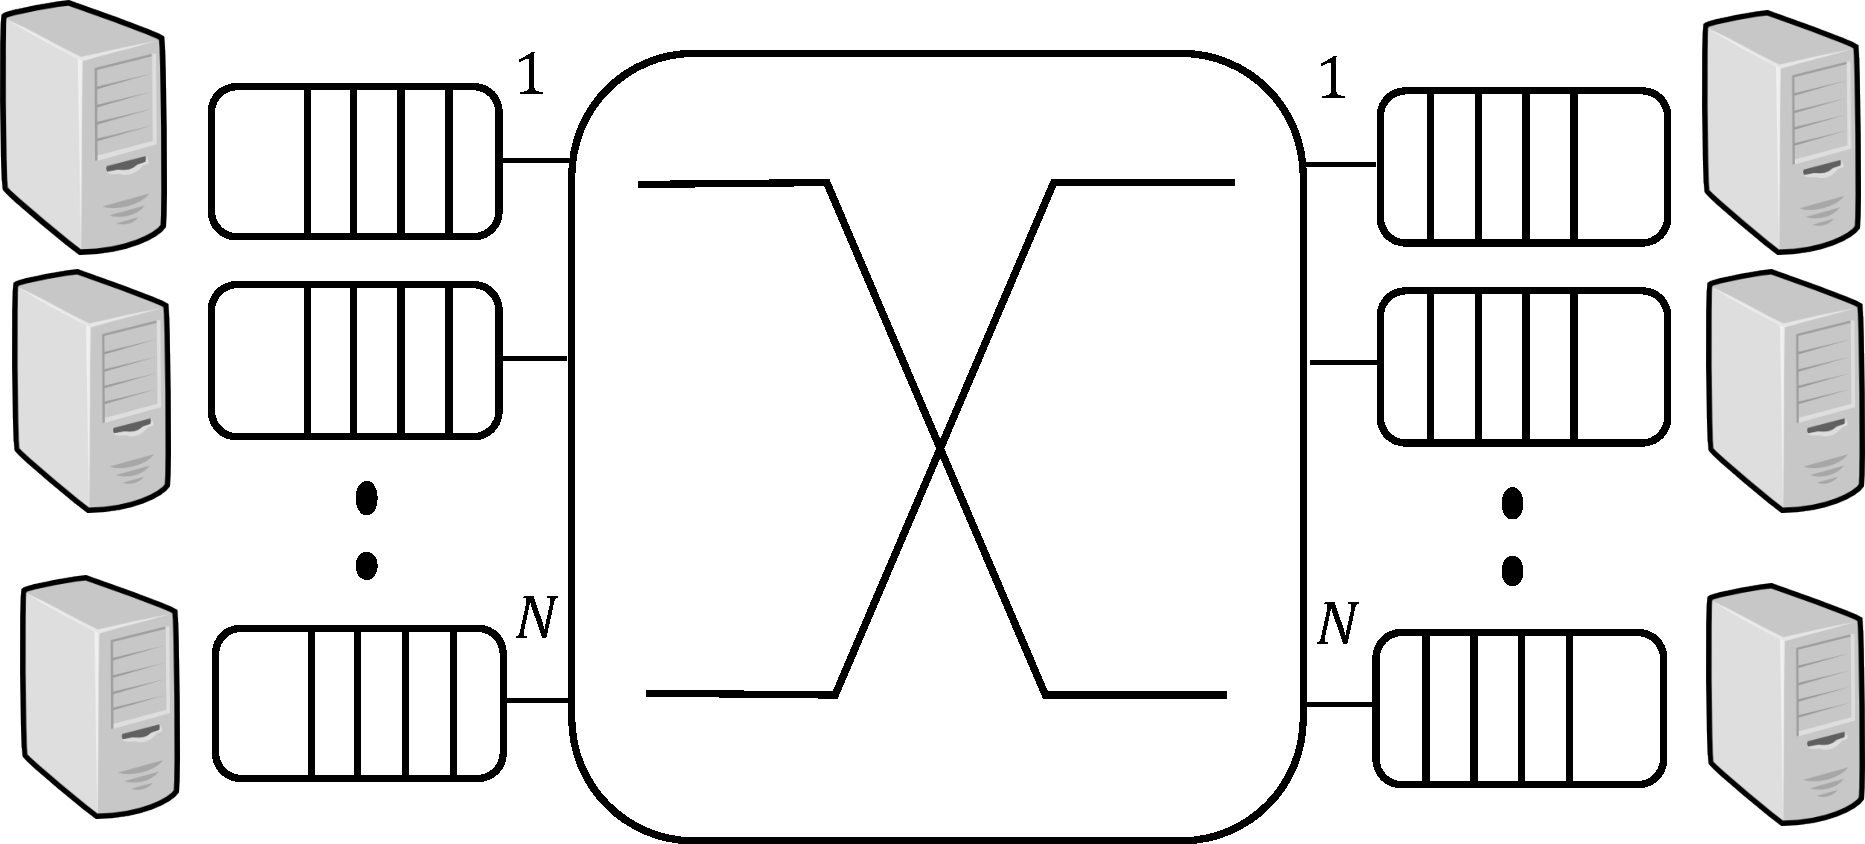
\includegraphics[width=0.55\textwidth]{Chapter2/Figures/pfabricdcn}
	\caption{Datacenter fabric abstraction as a giant switch}
	\label{fig:pfabricdcn}
\end{figure}

\subsubsection{Ideal flow scheduling in DCN}
Assuming that the fabric can sustain maximum throughput and that flows compete against each other only at ingress and egress interfaces, the optimal solution to minimize the flow completion time can be found solving a NP-hard problem known as \textit{sum-multicoloring}. Nevertheless, a simpler greedy algorithm exists and it has been proven to be very close to the optimum. Authors referred to this algorithm as the \textit{Ideal} algorithm and used it as a baseline for the evaluation of pFabric.  Briefly, it consists in a maximal flow scheduling, where at every new flow arrival or depart, flows are sorted in ascending order of data remaining up to their completion and served with this order. Flows are not served until there is another flow with less data remaining traversing the same ingress or egress port. Despite being a simplified model, still the \textit{Ideal} algorithm is a valid benchmark for any design that targets flow completion time minimization, since it is a sort of best case latency at a desired level of load and over an ideal interconnection network. \\
At this point, pFabric showcased that it is possible to achieve nearly ideal performances in a distributed way, treating each interface on its own with local scheduling decisions and simultaneously rely on minimal transport strategies. In particular, their work can be summarized in the following key aspects. \\
\begin{enumerate}
	\item \textit{Knowledge of flow requirements}. It is assumed to know at transport layer flow sizes or flow deadlines for deadline-constrained traffic. 
	\item \textit{Prioritization}. Schedulers in the network are priority schedulers. Depending on the scheduling objective, the packets encode with a priority a different metric, on which the scheduler choices are based on. For example, to approximate SRPT on every single link, the priority may indicate the amount of bytes still to transmit for a given flow. Packets are dequeued and dropped according to their priority. 
	\item \textit{Simple rate-control}. Rate control at end hosts is minimal and aims just to avoid persistent congestion. In fact, contrary to DCTCP (Sec. \ref{sec:dctcp}), even if queue sizes grow, only the performance of few long flows is significantly impacted, since it is used a detailed prioritization mechanism both for packet transmission and drops. Some shrinkage to standard TCP have been described to realize such minimalistic transport.
\end{enumerate}
 
 \subsubsection{Approximate optimality with priority queues}
As already mentioned, implementing such a prioritization scheme on available commodity devices is very challenging and for sure would require hardware modifications. The interested reader could find a possible digital design in the paper of pFabric. The same source, however, provided also a straightforward solution readily deployable with current switches. The idea is to coarse the granularity of the scheduler by adopting only a finite number of priority levels. Then, packets with different priorities are enqueued in corresponding priority queues (PQs) and handled with traditional network schedulers (SP, WRR, WFQ, etc.). In pFabric it is employed a Strict Priority (SP) scheduler, but in general other choices are not precluded \cite{mqecn}. In short, LAS and SRPT schedulers, as well as other disciplines, can be emulated by tagging packets with a priority label and leveraging separated queues in network interfaces. The typical number of priority queues available in datacenter switches ranges between 2 and 8, albeit it often occurs that some of them are reserved --- more details in Sec. \ref{sec:pias}. Of course, increasing the number of PQs results in better approximation of the ideal scheduling, that implicitly would correspond to having an infinite number of PQs. In fact, the ideal scheduler directly compares each other all priorities of the packets in the buffer.

Finally, the FCT gain obtained with this system largely depends on the way flows are clustered in priority levels. This underlies the need of a careful tuning of a set of thresholds which split packets among the priorities available. A dedicated section of this work illustrates some criterion to choose them (\S \ref{sec:thresholds}). 

\end{subsection}

\begin{subsection}{PIAS: the reference model}
	\label{sec:pias}
	The next step with respect to pFabric as well as the starting point of this work is PIAS: Practical Information-Agnostic Scheduler \cite{pias}. This proposal is the first which addresses the scheduling problem without the assumption of an exact prior knowledge about the flow size. Instead, PIAS tries to mimic a LAS scheduler exploiting the sole knowledge of the distribution of flow sizes rather than their precise values. Surprisingly, when compared to pFabric it delivers very similar performances for short flows, that are the more critical ones (the gap is within 4.9\%). At the same time, however, PIAS preserves ease of deployment with the current switch hardware and the standard distributed congestion-control algorithms.
	Summarizing, the two main design principles of PIAS are:
	
	\begin{enumerate}
		\item \textit{Flow-agnostic}. It requires only the knowledge of DC-wide flow size distribution, which can be easily estimated once and updated dynamically. Authors do not account for any heterogeneity of the distribution across different racks \cite{facebook_dcn}, in what the problem would become quite difficult ot treat with analytical methods. Also dynamic changes of the distribution along time have been ignored, but the architecture is flexible enough to adapt to this case.
		\item \textit{Low complexity}. It should be compatible with legacy TCP/IP protocol stack and readily deployable without touching the hardware of existing devices.
	\end{enumerate}

	\begin{figure}
		\centering
		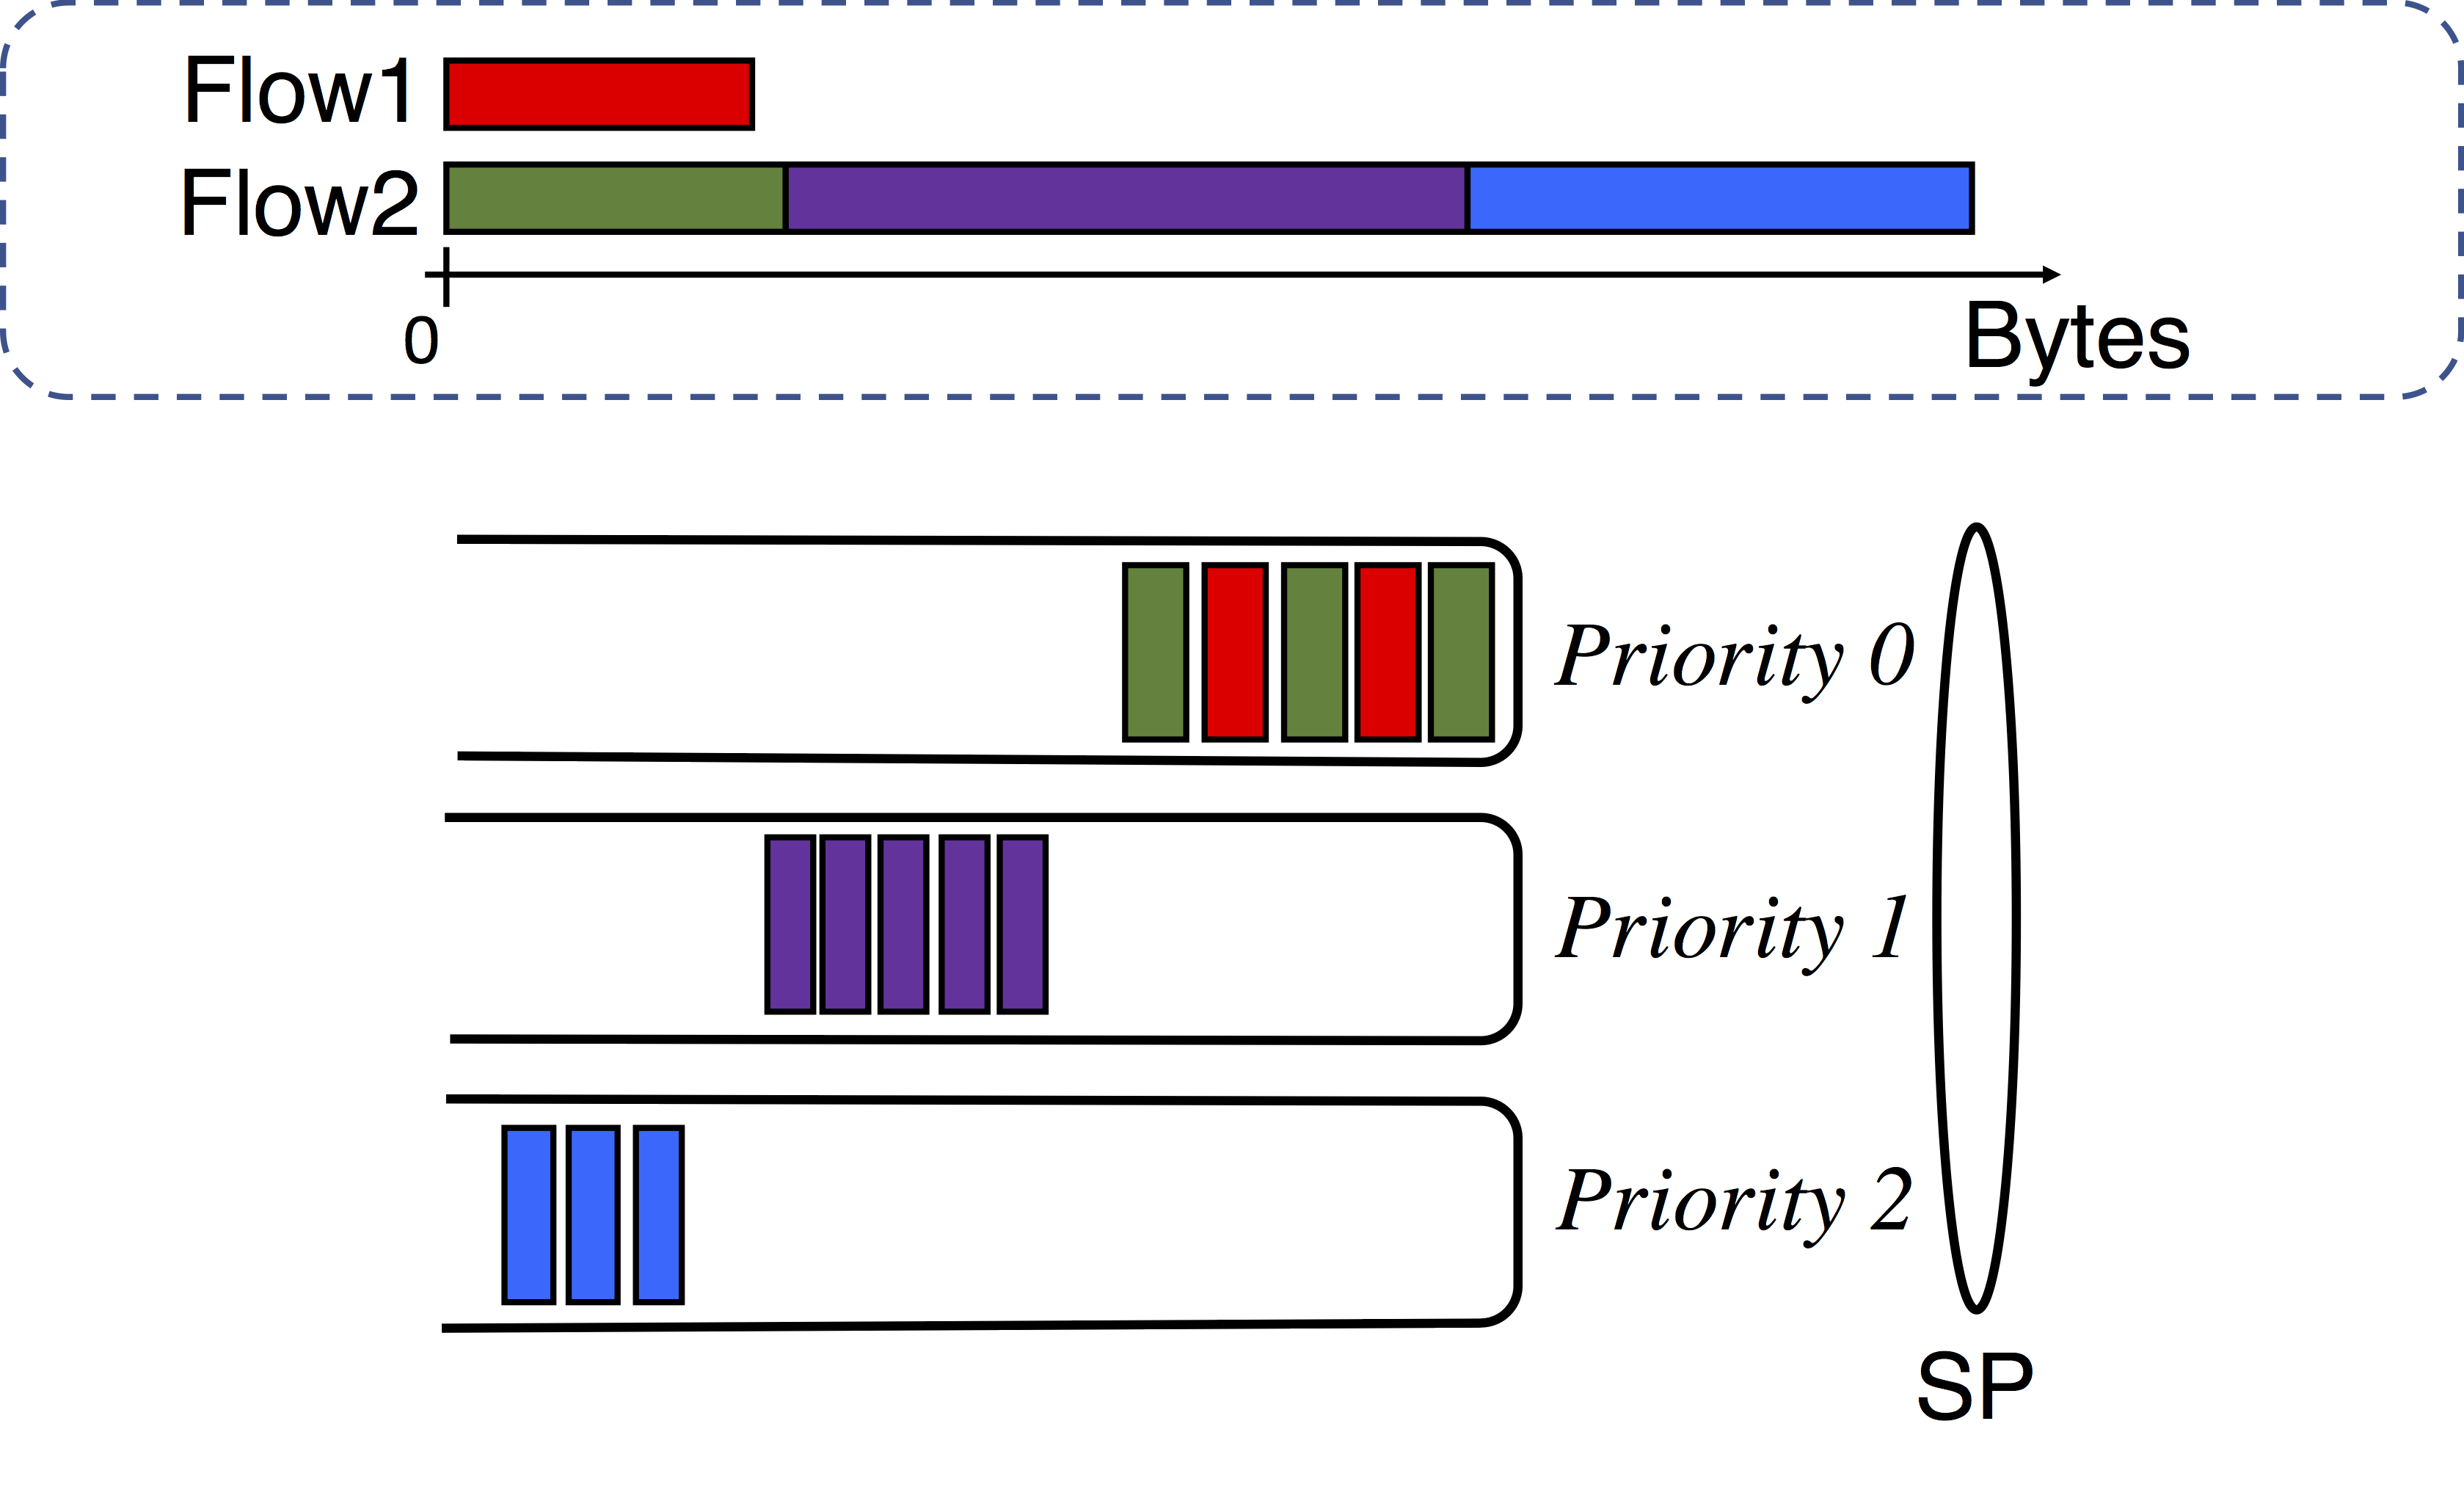
\includegraphics[width=0.5\textwidth]{Chapter2/Figures/pias_scheme}
		\caption{PIAS overview}
		\label{fig:pias_scheme}
	\end{figure}

	PIAS embraces a \emph{Multi Level Feedback Queue} (MLFQ) mechanism to resemble the LAS policy. MLFQ essentially apportion flows in a finite number of priority queues as proposed in pFabric, but in absence of flow size information flows are dynamically moved across priority queues. In more details, each packet of a given flow is mapped to a priority level, inversely proportional to the bytes it has already sent since its beginning. All flows starts with the highest priority, then longest flows are progressively demoted to lower priorities. Packets of same priority are buffered in the corresponding PQ according to a First-In First-Out (FIFO) order, while packets belonging to different priority queues are scheduled in Strict Priority (SP). In this way, packets belonging to short flows are always prioritized over those belonging to long flows, mimicking LAS but without incurring in the complexity of its implementation, which would require many comparisons. Figure \ref{fig:pias_scheme} clarifies the demotion mechanism. $\text{\emph{Flow}}_1$ is a mice flow and it is entirely served at the highest priority, whereas $\text{\emph{Flow}}_2$ is an elephant flow and it is gradually de-prioritized up to the last PQ. Notice that differently from pFabric, all flows traverse highest priorities in their initial lifetime, since their size is initially obscure. Hence, longer jobs constitute a small impairment for short ones, that motivates the gap with pFabric.

A key point for this kind of systems is how to choose the demotion thresholds. In fact, especially when few queues are available, an unbalanced threshold setting may lead to severe performance degradation. On one hand, thresholds too small cause premature flow demotion and delays for short flows that get mixed with long flows, on the other hand if the thresholds are too large, medium and elephant flows overstay in high priorities, resulting again in worse FCT for delay sensitive flows. The next section will present simple heuristics and a more refined optimization to find the set of thresholds.
\end{subsection}

\section{The problem of demotion thresholds}
The same authors of PIAS proposed a queueing model to mathematically describe the dynamics of the system. It has to be remarked that the queueing model captures only the average flow completion time on a single interface. Therefore, it is assumed that the flow size distribution is homogeneous over the datacenter fabric so that bottleneck links observe all the same distribution. With this assumption, the average FCT over the whole fabric is just a linear rescaling of the average FCT on a single link, therefore the performance index of any set of thresholds obtained with the model is meaningful for the whole DCN as well. 

In the following of this section, first it is formalized the queueing model along with its parameters, then it is formulated a non-linear minimization problem that can be used to optimize demotion thresholds. Finally, two other trivial heuristics for threshold assignment are reviewed.

\subsection{Stochastic queueing model}
\begin{figure}
	\centering
	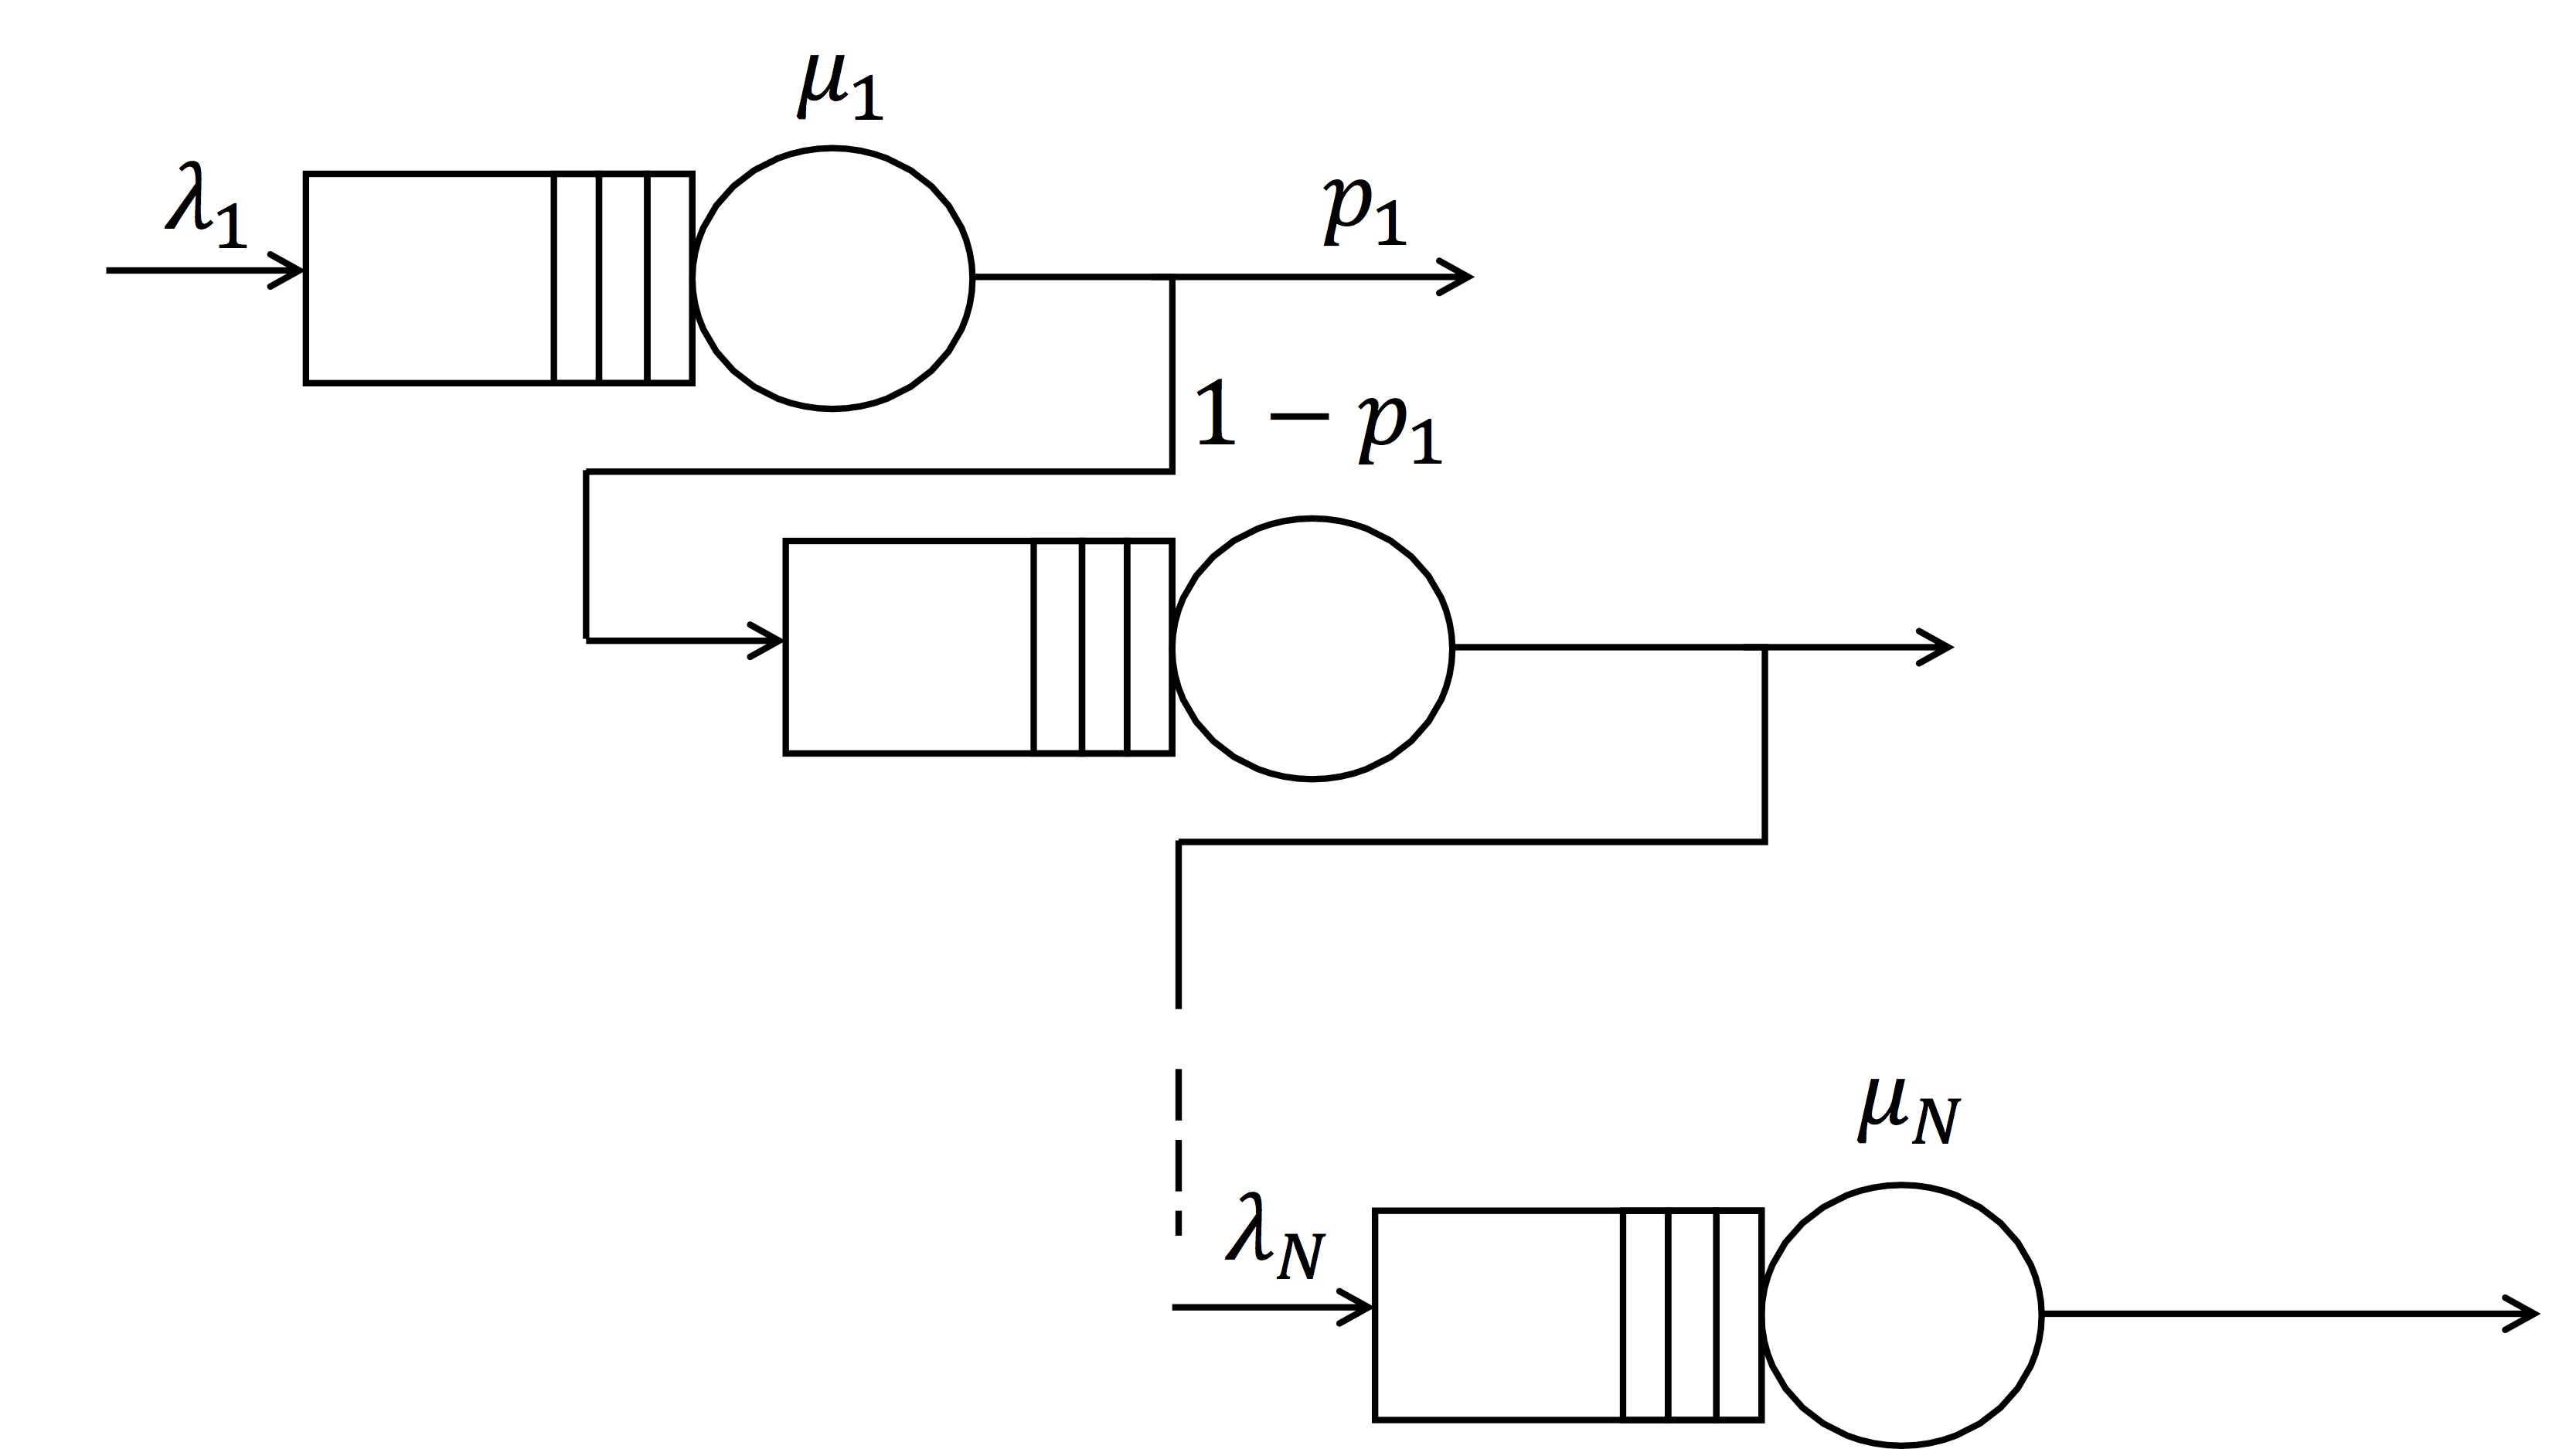
\includegraphics[width=0.5\textwidth]{Chapter2/Figures/pias}
	\caption{Queueing model}
	\label{fig:pias}
\end{figure}

The system, shown in Figure \ref{fig:pias}, is thought as a tandem of $N$ subsequent M/M/1 queues.  The customers are flows of size $X$ extracted from a given distribution with cumulative function $F(x)$ and arriving according to a Poisson process of intensity $\lambda$. Queues are lazy and able to serve at most a maximum amount of bytes for each flow, that depends on the demotion thresholds. When customers enter the system they are initially served by the first queue, then either they leave the system if all of their bytes have been served, or they are demoted to subsequent queue, up to queue $N$. \\ 
Let be $Q_p(1 \le p \le N)$ the $N$ priority queues. Denote with $\alpha_i$ the threshold after which a flow changes its priority from $i-1$ to $i$, where higher priorities correspond to lower indexes and $i \in [0,N]$. The upper threshold is always set to $\alpha_N = \infty$ so that all the largest flows stay in the last queue, similarly $\alpha_0 = 0$ for simplicity. Each queue $Q_i$ can serve at most $\alpha_i - \alpha_{i-1}$ bytes of any customer. In the real MLFQ system (Sec. \ref{sec:pias}), all queues of a given port are orchestrated by a Strict Priority (SP) scheduler, however this would make the queues dependent on each other complicating the analysis. To avoid the issue, the queues are treated as if they are independent and their priority hierarchy is taken into account by adjusting their drain rate $\mu_i$. In fact, if $\mu$ is the overall link capacity, subsequent queues in the tandem are assigned a drain rate $\mu_i$ equal to the residual bandwidth left after servicing previous queues. In practice, denote with $\rho_i$ the load insisting on $Q_i$, then 
\begin{equation}
\mu_i = \mu \prod_{j=1}^{i-1} (1-\rho_j)
\end{equation}
Next, for the sake of conciseness let's indicate with $\theta_i \triangleq F(\alpha_{i}) - F(\alpha_{i-1})$ the probability that a new flow has size in $[\alpha_{i-1}, \alpha_{i})$ and abbreviate with the notation $\bar{F}(x) = 1 - F(x)$ the survival function of $X$. The target is to derive the subsequent arrival rates $\lambda_i$.
After service in queue $i$, a customer leaves the system with a probability $p_i$, that depends on flow size distribution. In fact, customers who leaves the systems after the $i$-th queue are the flows with size in $[\alpha_{i-1}, \alpha_{i})$, among those with size in $[\alpha_{i-1}, \infty)$. Therefore, $p_i$ can be expressed renormalizing the probability $\theta_i$ as:
\[
p_i = \theta_i \mslash \bar{F}(\alpha_{i-1})
\]
Consequently, from the definition of $\theta_i$
\[ 	
1-p_i = \bar{F}(\alpha_{i}) \mslash \bar{F}(\alpha_{i-1}) 
\]
If the system is stable, the arrival rate of queue $i$ is nothing else than the output rate
of queue $i-1$, weighted by the probability of remaining in the system. 
Therefore: 
\[
\lambda_i = \lambda_{i-1} (1-p_{i-1})
\]
By iterative substitution it is possible to get a general expression for every $\lambda_i$ that depends only on the flow generation intensity $\lambda$ and the arrival rate at the previous queue $\lambda_{i-1}$. Indeed:
\begin{align*}
&\lambda_1 = \lambda \qquad \qquad & 1-p_1 &= \bar{F}(\alpha_1) / \bar{F}(\alpha_0) = \bar{F}(\alpha_1) \\
&\lambda_2 =  \lambda_1 (1-p_1) = \lambda \bar{F}(\alpha_1)  \qquad \qquad & 1-p_2 &= \bar{F}(\alpha_2) / \bar{F}(\alpha_1) \\
&\lambda_3 =  \lambda_2 (1-p_2) = \lambda \bar{F}(\alpha_2)  \qquad \qquad & 1-p_3 &= \bar{F}(\alpha_3) / \bar{F}(\alpha_2) \\
& \cdots \qquad \qquad & \cdots &
\end{align*}
In general:

\[
	\lambda_{i} = \lambda \bar{F}(\alpha_{i-1})
\]
Finally, this rate refers to flow arrivals, whereas thresholds $\alpha_i$ are expressed either in bytes or in packets, because they serve for demotion. It is simple to obtain the byte arrival rate by scaling $\lambda_i$ (flows/sec) of the average traffic size produced by these flows on queue $i$. Remember that due to the demotion mechanisms, customers of each queue are truncated versions of the original flows, whose size ranges in $(0, \alpha_{i}-\alpha_{i-1})$. and that, subsequent priority queues observe a flow distribution truncated above $\alpha_{i-1}$. \\
It is needed to compute $\mathbb{E}[L_i]$, the average length of customers served in queue $i$. It holds:

\begin{equation}
\label{load-on-pqi}
\mathbb{E}[L_i]=
\underbrace{\int_{\alpha_{i-1}}^{\alpha_i}(x-\alpha_{i-1})f(x)dx}_{\text{(i)}} +
\underbrace{(\alpha_{i}-\alpha_{i-1})\int_{\alpha_i}^{\infty}f(x)dx}_{\text{(ii)}}
\end{equation}

\begin{itemize}
	\item[(i)]Traffic generated by flows with sizes in $[\alpha_{i-1},\alpha_{i})$
	\item[(ii)] Traffic generated by flows larger than $\alpha_{i}$
\end{itemize}
Define the truncated probability density function seen by queue $i$ as:
\[
f_i(x) = f(x) \mslash \bar{F}(\alpha_{i-1})
\]
It holds:
\begin{equation}
\lambda_i =   \lambda \, \bar{F}(\alpha_{i-1}) \frac{\mathbb{E}[L_i]}{\bar{F}(\alpha_{i-1})} = \lambda \, \mathbb{E}[L_i]
\end{equation}

\begin{table}%[tb!]
	\label{tab:queuingmodel}
	\footnotesize 
	\centering
	\resizebox{0.6\textwidth}{!}{
		\begin{tabular}{c l l }
			\hline
			\textbf{Variable} & \multicolumn{1}{c}{\textbf{Description}}  \\ \hline \hline
			$Q_i$ & Priority queue $i$ \\ \hline
			$N$ & Number of priorities $i$ \\ \hline
			$X$ & Flow size \\ \hline
			$F(x)$ & Flow size c.d.f. \\ \hline
			$f(x)$ & Flow size p.d.f.  \\ \hline
			$\lambda_i$ & Packet arrival rate at PQ $i$  \\ \hline
			$\mu_i$ & Drain rate of PQ $i$ \\ \hline
			$\rho_i$ & Average load on $Q_i$ \\\hline
			$L_i$ & Customer size at PQ $i$   \\\hline
			$T_i$ & Waiting time at PQ $i$  \\\hline 
			$\alpha_i$ & Demotion threshold from $Q_{i-1}$ to $Q_i$ \\ \hline
			$p_i$ & Probability that a flow leaves after $Q_i$ \\ \hline 
			\hline
	\end{tabular}
}
	\caption{Variables of the model.}
\end{table}

Summarizing, it was possible to write down all arrival rates $\lambda_{i}$ and all draining rate $\mu_i$ as function of the flow size distribution and the set of thresholds $\alpha_i$. A summary of all quantities that have been defined is provided in Table \ref{tab:queuingmodel}.
These parameters are sufficient to express the average sojourn time on a single link, so to characterize the performance of PIAS. The average sojourn time on queue $i$ which comprises the average waiting and serving time is given by the well-known formula for M/M/1 queues:
\begin{equation}
\label{mm1}
\mathbb{E}[T_i] = \dfrac{1}{\mu_i-\lambda_i}
\end{equation}
The M/M/1 model holds for every subsequent queue. This follows from Burke's theorem \cite{burke}, that states that the outgoing process of an M/M/1 queue is a Poisson process. Thus, cascaded queues still observe a Markovian arrival process. \\
Finally, the total average sojourn time in the tandem of $N$ queues is just a linear combination of $\mathbb{E}[T_i]$, where the coefficient that weight the individual sojourn times at any priority queue are the probabilities that a flow shall traverse the same PQ.
\begin{equation}
\mathcal{T} = 
\sum_{i=1}^{N} \theta_i \sum_{j=i}^{N}\mathbb{E}[T_j]
\end{equation}
Thus, given the flow size distribution it is possible to easily compute the system performance according to the model yet presented. 

\subsubsection{Optimal thresholds}
\label{sec:pias-queueing-model}
Plainly, it follows that the \textit{optimal} thresholds $\alpha_i$ can be derived solving the non-linear minimization of $\mathcal{T}$. Notice that they are easily obtainable once all $\theta_i$ are known as 

\[
\alpha_i = F^{-1}(\sum_{j=1}^{i}\theta_j)
\]
Hence, it is possible to solve in $\theta_i$.
\begin{equation}
\label{eq::costfunction}
\begin{aligned}
&\underset{\{\theta_i\}}{\text{min}} \quad  & &\mathcal{T} = 
\sum_{i=1}^{N} \theta_i \sum_{j=i}^{N}T_j \\
&\text{subject to} \quad  & &\theta_i \ge 0 \qquad \qquad \qquad \forall i \in [1,N]  \\
& & & \sum_{i=1}^{N} \theta_i = 1 
\end{aligned}
\end{equation}

\subsection{Greedy threshold assignment}
\label{sec:greedy-thresh}
In order to verify the actual gain obtained with optimal demotion levels, it is practical to compare it against simpler greedy strategies for thresholds assignment. Another reason motivating such alternatives is that when the number of priority levels increases ($N$>3) the solution to the previous optimization is very time consuming, since the problem is non-linear and non-convex. In chapter \ref{ch4} it is provided a breakdown which shows the CPU time spent for computing the optimal demotion thresholds through a meta-heuristic algorithm. 
Having a significant slow-down for the solution to converge deteriorates the reactiveness of the MLFQ scheduler in the case of a sudden change in the flow size distribution. As a consequence, the system would operate for long using thresholds mismatched with respect to the flow distribution.

Two intuitive approach are considered for fast threshold computation: Equal Split (ES) and Load Split (LS). 
%Therefore, for initial tests, it has been more practical to use a simpler criterion: assign thresholds so that the traffic load is equally distributed among available queues. \\

\subsubsection{Equal Split (ES-N)}
The \textit{Equal-Split} method slices the flow size distribution uniformly in $N$ percentiles. The resulting thresholds are the corresponding quantiles:

\[
\alpha_{i} = F^{-1}\Big(\dfrac{i}{N}\Big), \qquad i=1,..,N-1
\]
It is easy to observe that this criterion may be largely sub-optimal depending on the shape of the flow size distribution. In the case of very sharped distributions short flows are demoted too early to lower priorities, while for heavy-tailed distributions, where high percentiles correspond to very long flows, latency sensitive flows remains mixed for long with elephant throughput-oriented streams.

\subsubsection{Load Split}
\emph{Load Split} is a technique where the thresholds are chosen in a way to control the amount of traffic fed in every priority queue.  The problem is easy to understand in the simple case of $N$=2 priority queues and a single threshold $\alpha$. Let $G(y)$ be the amount of traffic generated by flows with size less than $y$:
\[
G(y) = \int_{0}^y x f(x) dx
\]
The traffic on high priority queue $Q_0$ is derived as the sum of bytes generated by flows whose size is smaller than the threshold $\alpha$, and the bytes transmitted by flows larger than $\alpha$:
\[
\mathbb{E}[L_0] = \int_0^\alpha xf(x)dx+\int_\alpha^\infty \alpha f(x) dx=G(\alpha)+\alpha \bar{F}(\alpha)
\]
while the traffic on low priority queue is
\begin{equation*}
\mathbb{E}[L_1] =\int_\alpha^\infty (x-\alpha)f(x)dx=\mathbb{E}[X]-	\mathbb{E}[L_0]
\end{equation*}
Then, the traffic on the high priority queue can be controlled solving the following \textit{load-balance} equation:

\begin{equation}
\label{eq:main-gen}
\mathbb{E}[L_0] = \gamma \mathbb E[X] 
\end{equation}

A proper choice of $\gamma$ apportions to the high priority queue a fraction of the average total traffic $\mathbb{E}[X]  = \mathbb{E}[L_0] + \mathbb{E}[L_1]$. For example, if a perfect load balancing between the two queues is desired then it is set $\gamma = 1/2$.
Extending these equations to the general case of any number of priority queues is rather simple. The traffic on the $i$-th queue has the same expression of Eq\eqref{load-on-pqi}. It can be rewritten shortly with the notation just introduced:
\[
\mathbb{E}[L_i] = G(\alpha_i) - G(\alpha_{i-1}) + \alpha_i \bar{F}(\alpha_i) -\alpha_{i-1}\bar{F}(\alpha_{i-1})
\]
At this point, similarly to the simple case of two queues, it is enough to solve the following \emph{load-balance} equations iteratively for all $i = 1,..,N-1$:

\begin{equation}\label{eq:main-K-PQ}
\begin{cases}
\mathbb{E}[L_i] = \gamma_i \, \mathbb{E}[X],  \qquad &i = 1,..,N-1 \\
\sum_i \gamma_i = 1, \qquad &\gamma_i \in [0,1]
\end{cases}
\end{equation}
In fact, also in this case it holds $\sum_{i=1}^{N}\mathbb{E}[L_i] = \mathbb{E}[X]$.

\renewcommand{\qedsymbol}{\rule{0.5em}{0.5em}}
\begin{proof}
\textit{In the expansion of $\sum _{i=1}^{N}\mathbb{E}[L_i]$ at each step new terms simplify old terms. Since $\alpha_{\mathit{0}} = 0$ and $\bar{F}(\alpha_N) = 0$, it gives $\int_{0}^\infty x f(x) dx = \mathbb{E}[X]$}.
\small
\begin{align*}
	\sum\nolimits_{i=1}^{N}\mathbb{E}[L_i] &= \cdots + \cancel{G(\alpha_i)} - G(\alpha_{i-1}) + \cancel{\alpha_i \bar{F}(\alpha_i)} 
	-\alpha_{i-1}\bar{F}(\alpha_{i-1}) + G(\alpha_{i+1}) - \cancel{G(\alpha_{i})} \\ &+ \alpha_{i+1} \bar{F}(\alpha_{i+1})- \cancel{\alpha_{i}\bar{F}(\alpha_{i})} + \cdots 
	=G(\alpha_N) - G(\alpha_0) + \cancelto{0}{\alpha_N \bar{F}(\alpha_N)} -\cancelto{0}{\alpha_0\bar{F}(\alpha_0)} \\
	&=\mathbb{E}[X].
\end{align*}
\normalsize
\end{proof}

\section{A priority scheme with spatial-diversity}

\subsection{MLFQ with Spatial-Diversity}
In this chapter have been presented two attempts to approximate the optimal LAS and SRPT schedulers leveraging multiple priority queues, that are already present in all datacenter equipments. However, one limitation of this approach remains the scarce availability of priority queues in commodity switches. A large number of priority levels is demanded to better approximate the reference scheduling disciplines, in which $N \rightarrow \infty$ (Sec. \ref{sec:las}). Unfortunately, devices in modern DCNs are usually equipped with no more than 8 priority queues per port, whose majority are reserved for other purposes, like isolating different types of traffic. Indeed, several transport protocols may coexist in the same network, without necessarily being designed to be fair among them. Example of such transports are RDMA \cite{rdma}, DCTCP \cite{dctcp}, standard TCP and UDP. For this reason, it is plausible to assume to have at most $N=2$ priority queues as a realistic case. \\
Upon this understanding, the main proposal of this work is to evaluate the possibility to exploit the high degree of spatial diversity typically offered by DCN topologies to improve flow scheduling. Large DCN topologies are multilayer recursive Clos networks which offer a variety of equal-cost paths between racks. Precisely, in the simplest 2-layer Fat-Tree there are a number of paths proportional to the number of spines $K$ (Sec. \ref{sec:topology}). The key observation is that much like priority queues, different paths yet are a way for separating flows. In other words, the mechanism of priority demotion which shift the long flows across priority queues of a single interface, could be potentially applied at higher level as routing strategy over the switching fabric. Elephant flows would be physically segregated from mice flows, as they would be moved to different paths inside the switching fabric. Despite its simplicity, relevant works exploring this solution in the field of datacenter networks seem to be lacking. In more details, this contribution aims to integrate the spatial diversity property with the MLFQ scheduler. Consider a Leaf-Spine topology and focus on a single ToR switch. The interfaces from such a ToR towards all spines can be seen jointly as a unique big interface with $K$ times more priority queues than a port alone. The idea is better clarified in Fig.\ref{fig:sd-key-idea}.
\begin{figure}
	\centering
	\begin{subfigure}[htpb]{0.3\textwidth}
		\centering
		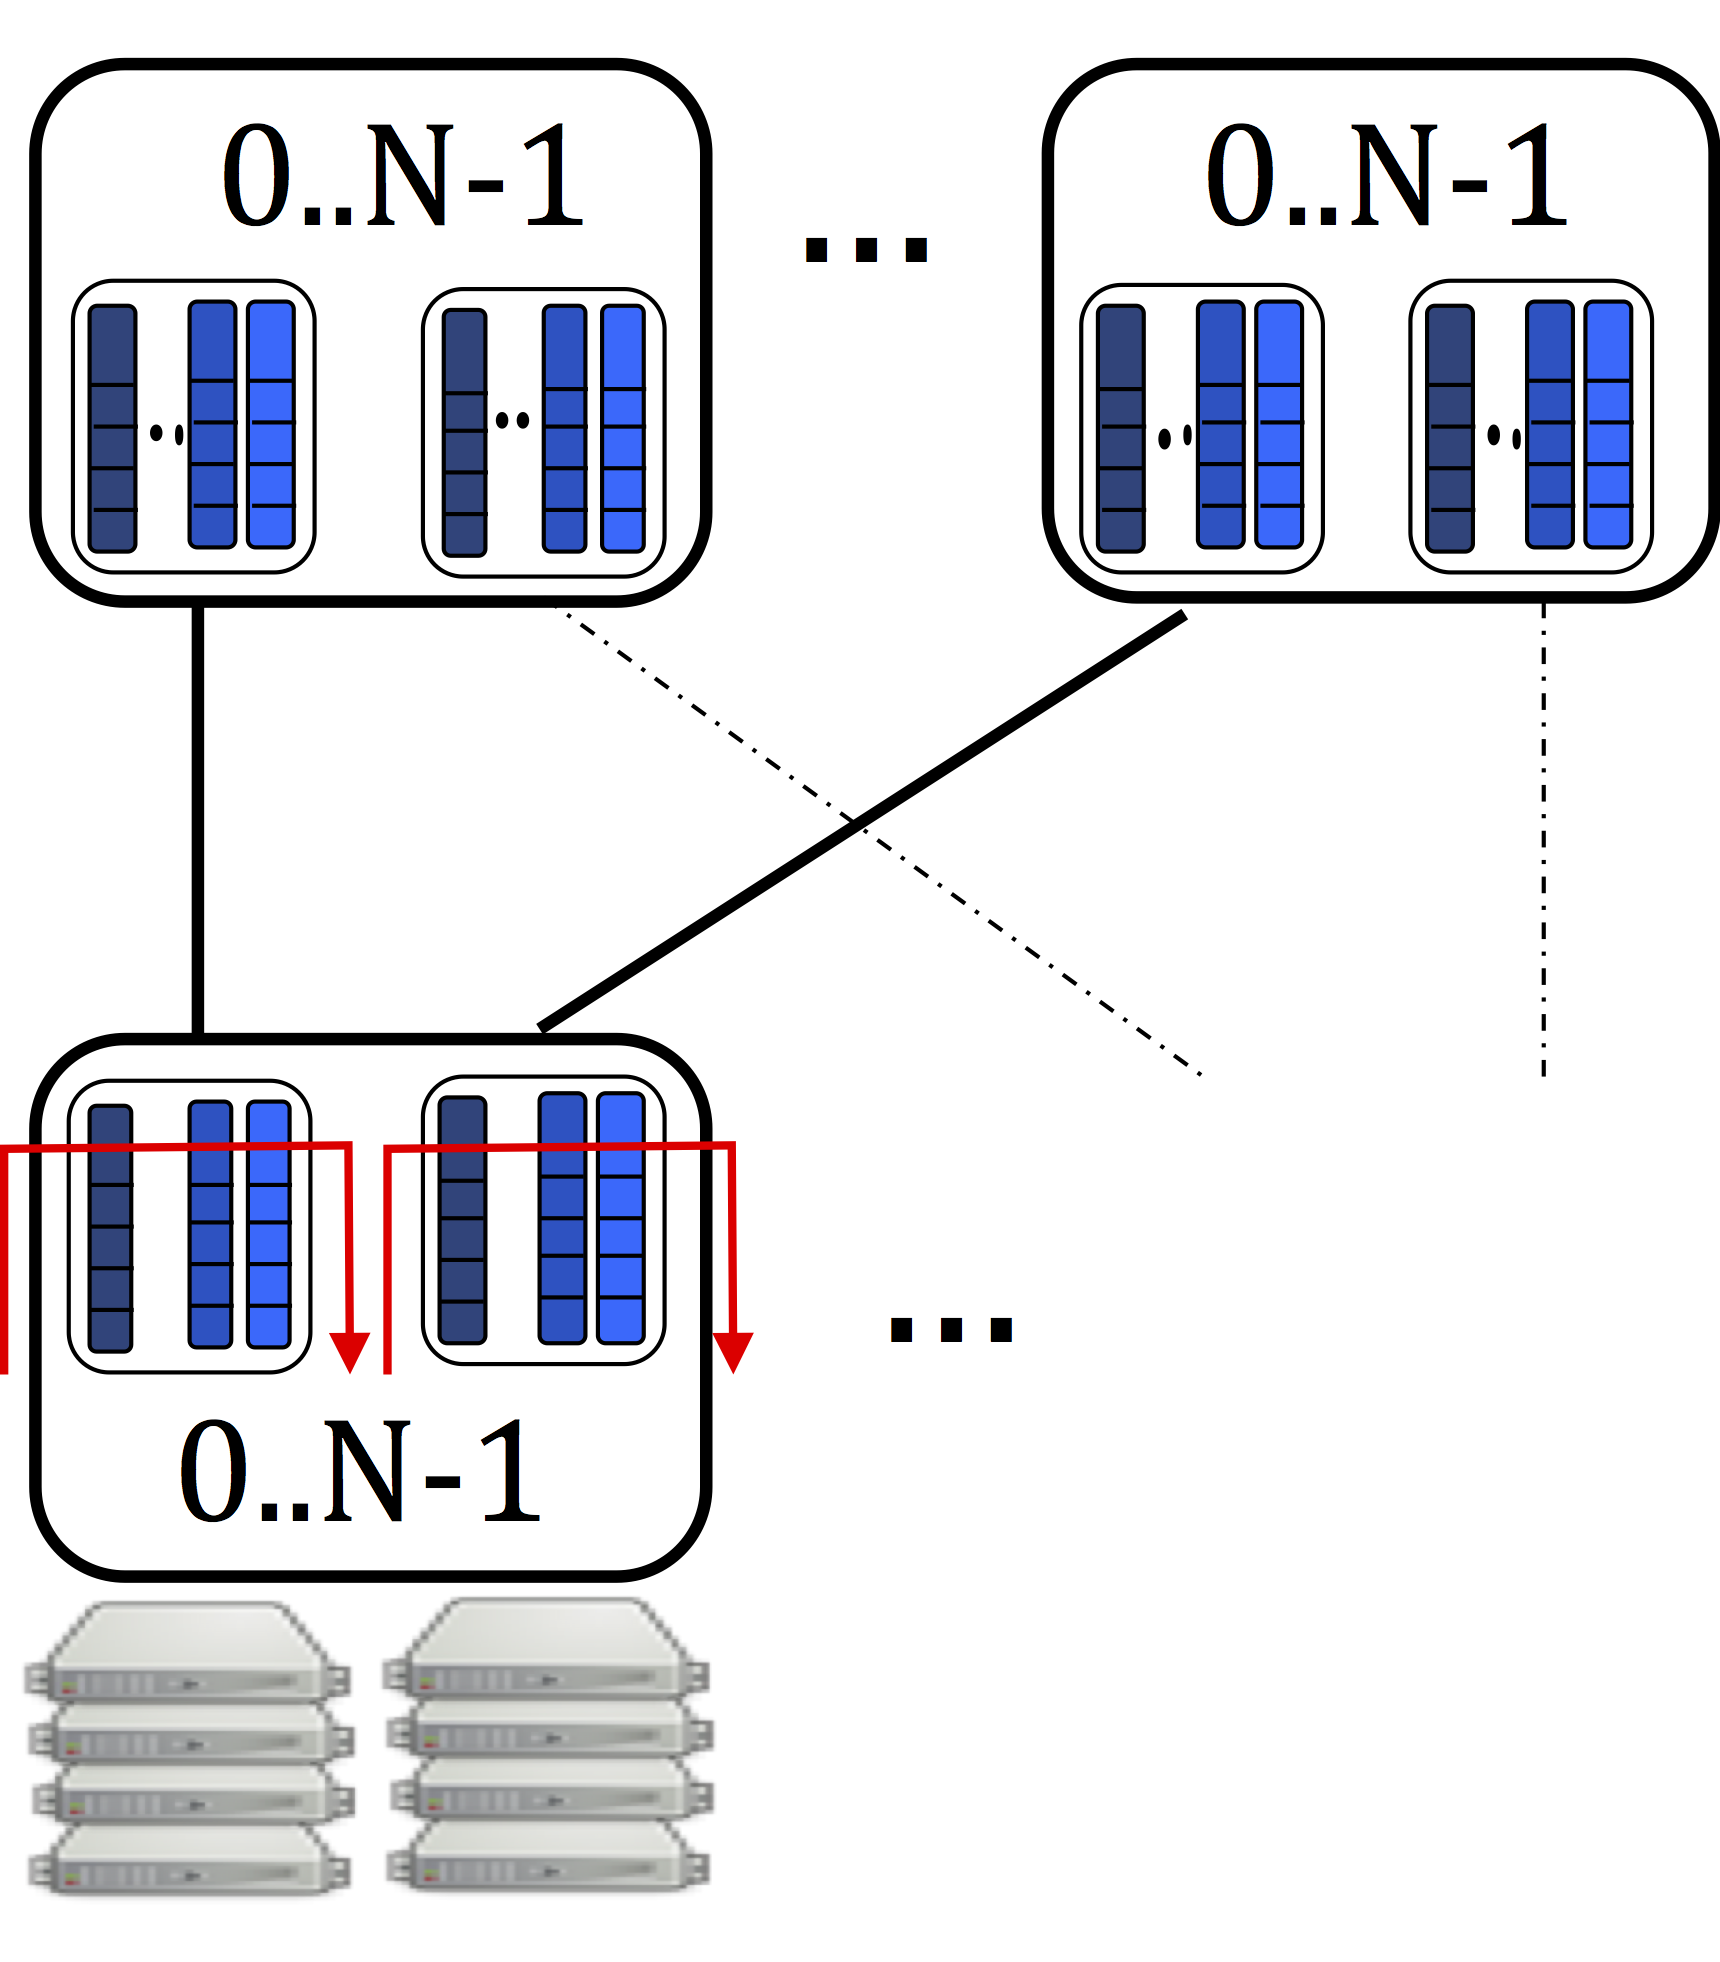
\includegraphics[width=\textwidth]{Chapter2/Figures/mlfq}
		\caption{MLFQ}
		\label{fig:sd-key-idea-mlfq}
	\end{subfigure}
	\hspace{0.2\textwidth}%
	\begin{subfigure}[htpb]{0.3\textwidth}
		\centering
		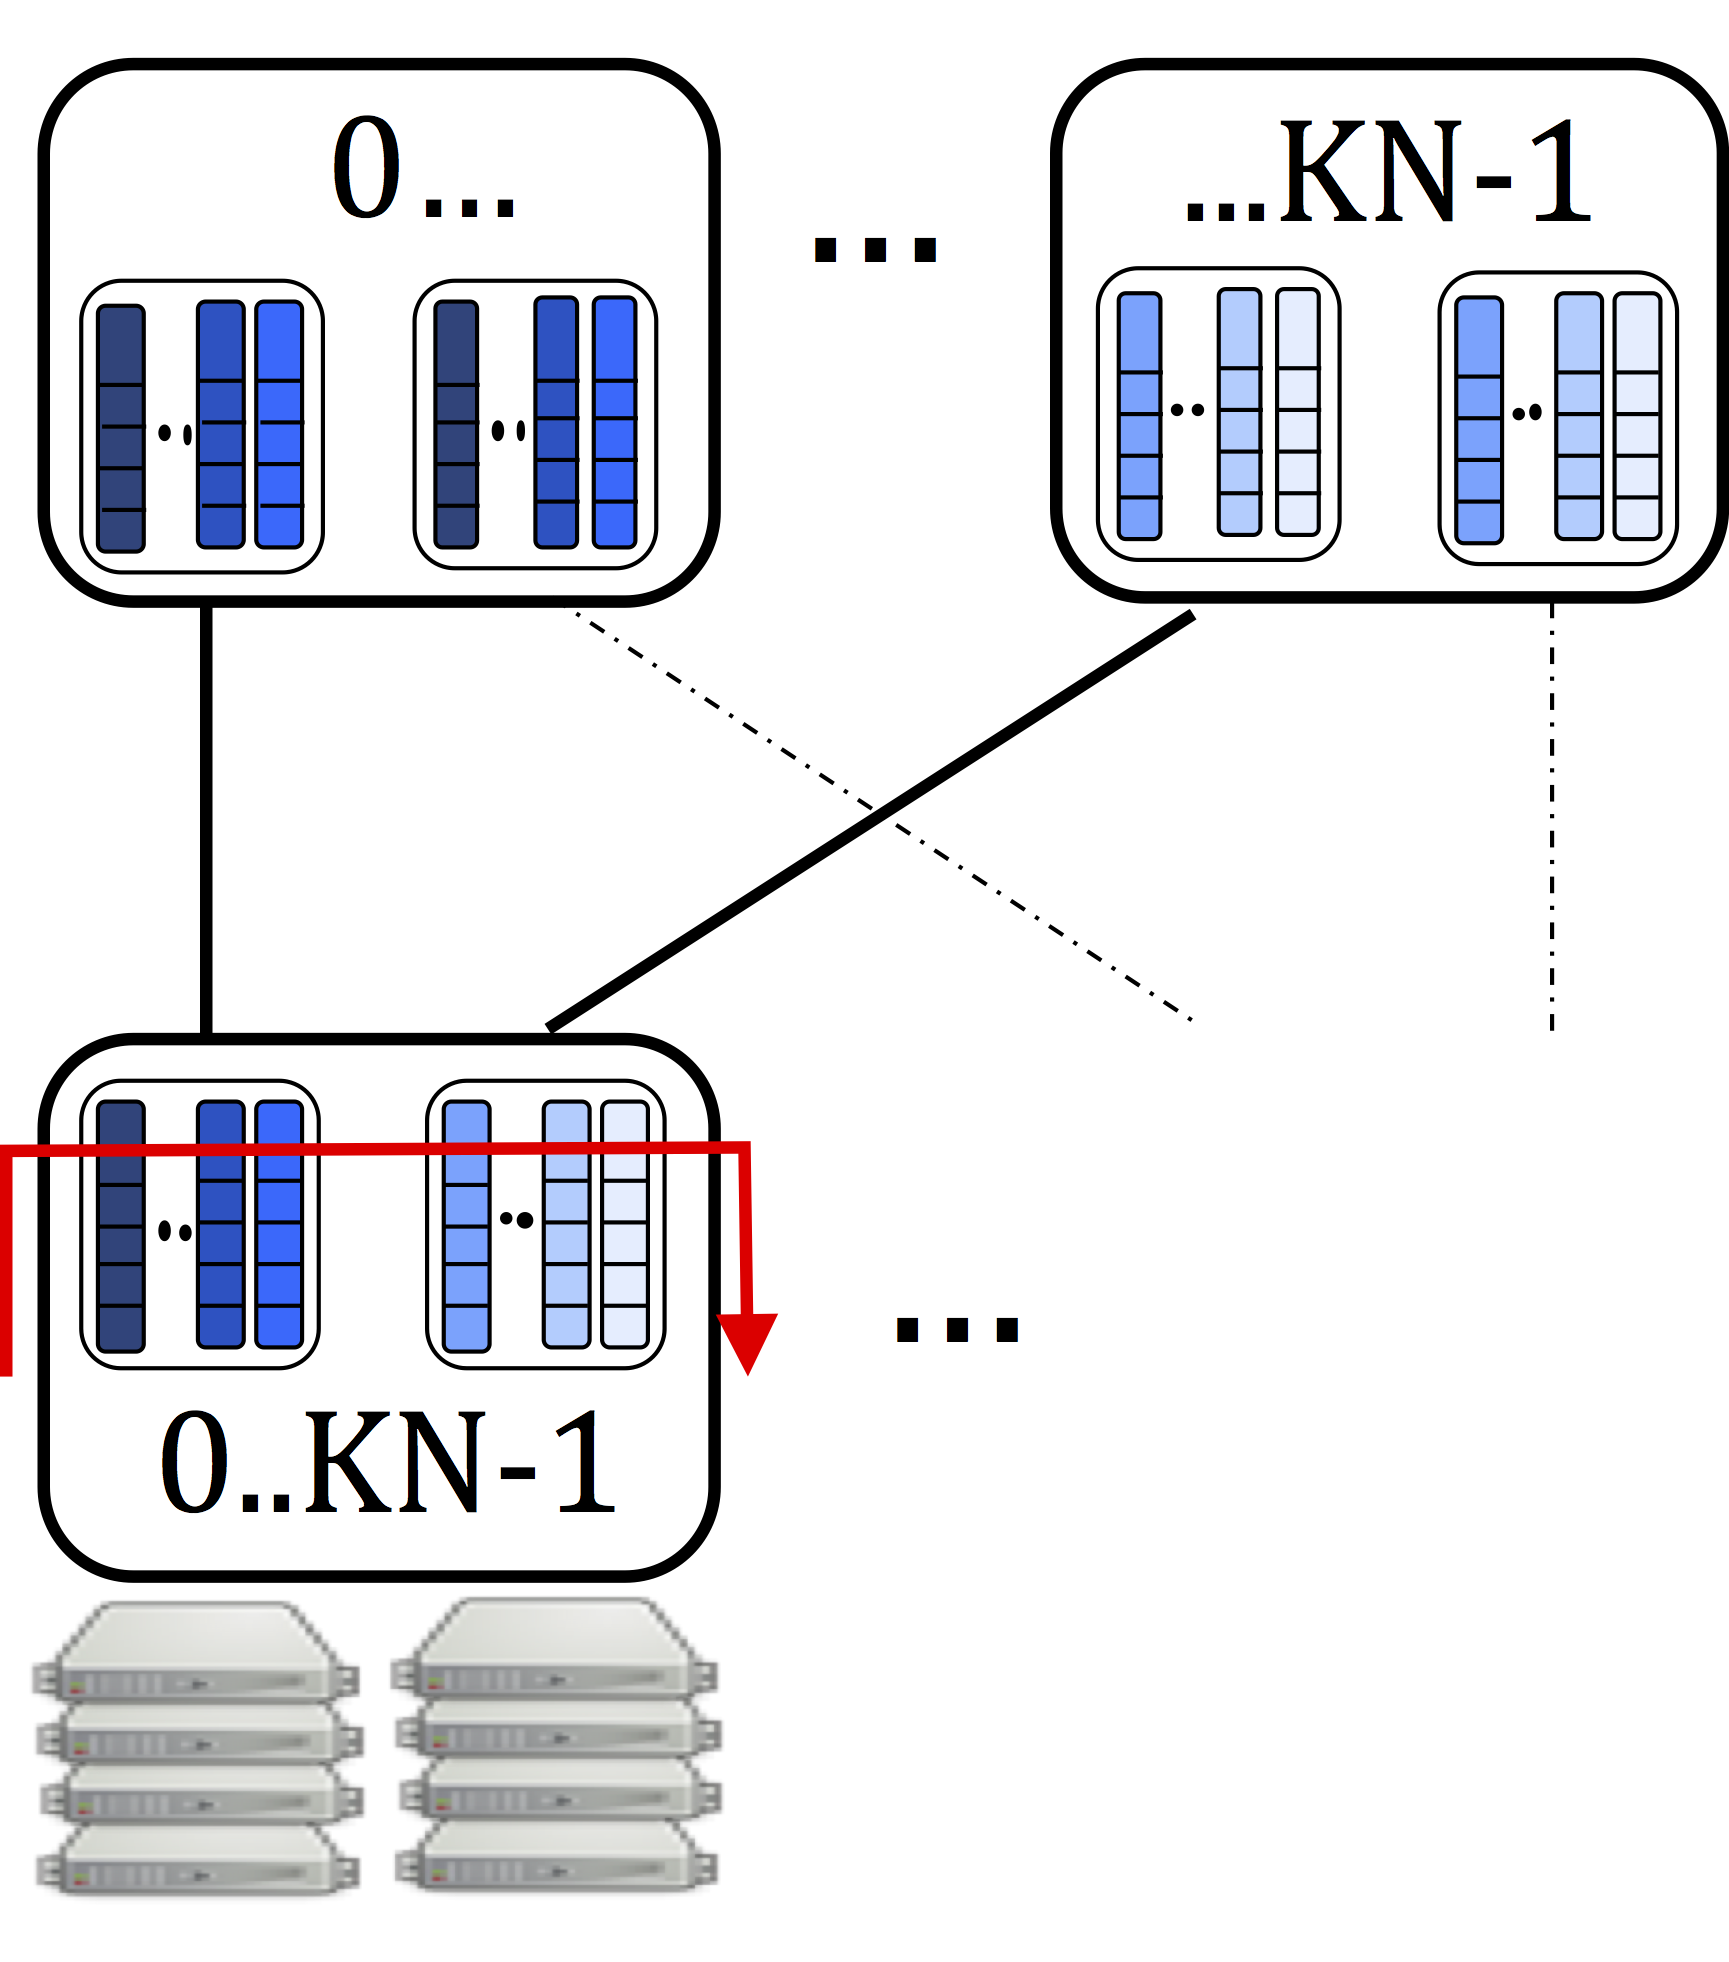
\includegraphics[width=\textwidth]{Chapter2/Figures/sdmlfq}
		\caption{SD-MLFQ}
		\label{fig:sd-key-idea-sdmlfq}
	\end{subfigure}
	\caption{Extension for spatial diversity.} %Red arrows indicate how queues are traversed during flow demotion. On each switch is reported the number of priorities it handles. Color scale is used to emphasize priority levels.}
	\label{fig:sd-key-idea}
\end{figure}
%Differently from 
The basic MLFQ (Fig.\ref{fig:sd-key-idea-mlfq}) focuses on the links individually and thanks to demotion moves flows, during their lifetime, across priority queues. Therefore, every interface handle the same priorities and flows are load balanced on different links independently from the prioritization mechanism. A standard technique for load balancing at flow-level is ECMP, which derives the next hop from the transport-layer tuple \texttt{\{IP ADDRESSES, PORTS, PROTOCOL ID\}}. Instead, this novel approach takes advantage of spatial diversity to extend the number of demotion levels beyond the limitation imposed by the PQs on a single interface. Interfaces from any ToR to the connected spines are virtually aggregated to offer a wider range of demotion levels. One new aspect of Spatially-Diverse MLFQ (SD-MLFQ) is that a demotion could imply to shift a flow from one path to another of equal-cost. In that light, the routing --- thus load balancing --- of flows on the Fat-Tree does depend on the priority. The spines can be seen as if they have a priority and a flow is moved both across queues and spines, effectively allowing a global resource exploitation for the demotion scheme. In other words, the routing policy over the fabric is not blind to the prioritization machinery, but smartly driven by the latter.  \\
A clear benefit of this scheme is that finer granularity in priorities is achieved even with few queues per port, at the price of a very limited implementation complexity.

\subsection{A queueing model extension for spatial-diversity}
\label{sec:complete-model}
PIAS model with added dimension for spatial diversity.
Proportional and equal splits for spatial diversiy

\chapter{The spatial diversity framework}
\label{ch:sdframework}
\section{Extending schedulers with spatial diversity}

In the previous chapter have been addressed the scheduling of jobs of variable size in relation to their probability distribution. Then, there were presented two attempts to approximate the optimal LAS and SRPT schedulers by leveraging multiple priority queues at network interfaces. However, one limitation of this approach remains the scarce number of such priority queues available in commodity switches. In particular, it was mentioned that a large number of priority levels is demanded to better approximate the reference scheduling disciplines, in which $N \rightarrow \infty$ (Sec. \ref{sec:las}). Unfortunately, devices in modern DCNs are usually equipped with no more than 8 priority queues per port, whose majority are reserved for other purposes, like isolating different types of traffic. Indeed, several transport protocols may coexist in the same network, without necessarily being designed to be fair with respect to each other. Example of such transports are RDMA \cite{rdma}, DCTCP \cite{dctcp}, standard TCP and UDP. For this reason, it is realistic to assume having at most $N=2$ priority queues in practical cases. \\
Upon this understanding, the main proposal of this work is to evaluate the possibility of exploiting the high degree of path diversity typically offered by DCN topologies, in order to improve the effectiveness of flow scheduling. Large DCN topologies usually are multilayer recursive Clos networks which offer a variety of equal-cost paths between racks. Precisely, in the simplest 2-layer Fat-Tree there are a number of paths proportional to the number of spines $K$ (Sec. \ref{sec:topology}). The key observation is that much like priority queues, different paths yet are a way for augmenting the granularity of prioritization and for separating flows with different QoS requirements. The novel paradigm being investigated aims to exploit \emph{spatial-diversity} to derive extra priorities and overcome the limitations in the maximum number of available PQs imposed by a single switch. Indeed, the mechanism of priority demotion, as proposed in PIAS, only shifts long flows across PQs of a single interface. Instead, we argue that the same demotion could be potentially applied at DC-level. Consider a Leaf-Spine topology and focus on a single ToR switch (Fig.\ref{fig:sd-key-idea}). The interfaces from such a ToR towards all spines can be seen jointly as a unique big interface with $K$ times more priority queues than a port alone.
\begin{figure}
	\centering
	\begin{subfigure}[htpb]{0.3\textwidth}
		\centering
		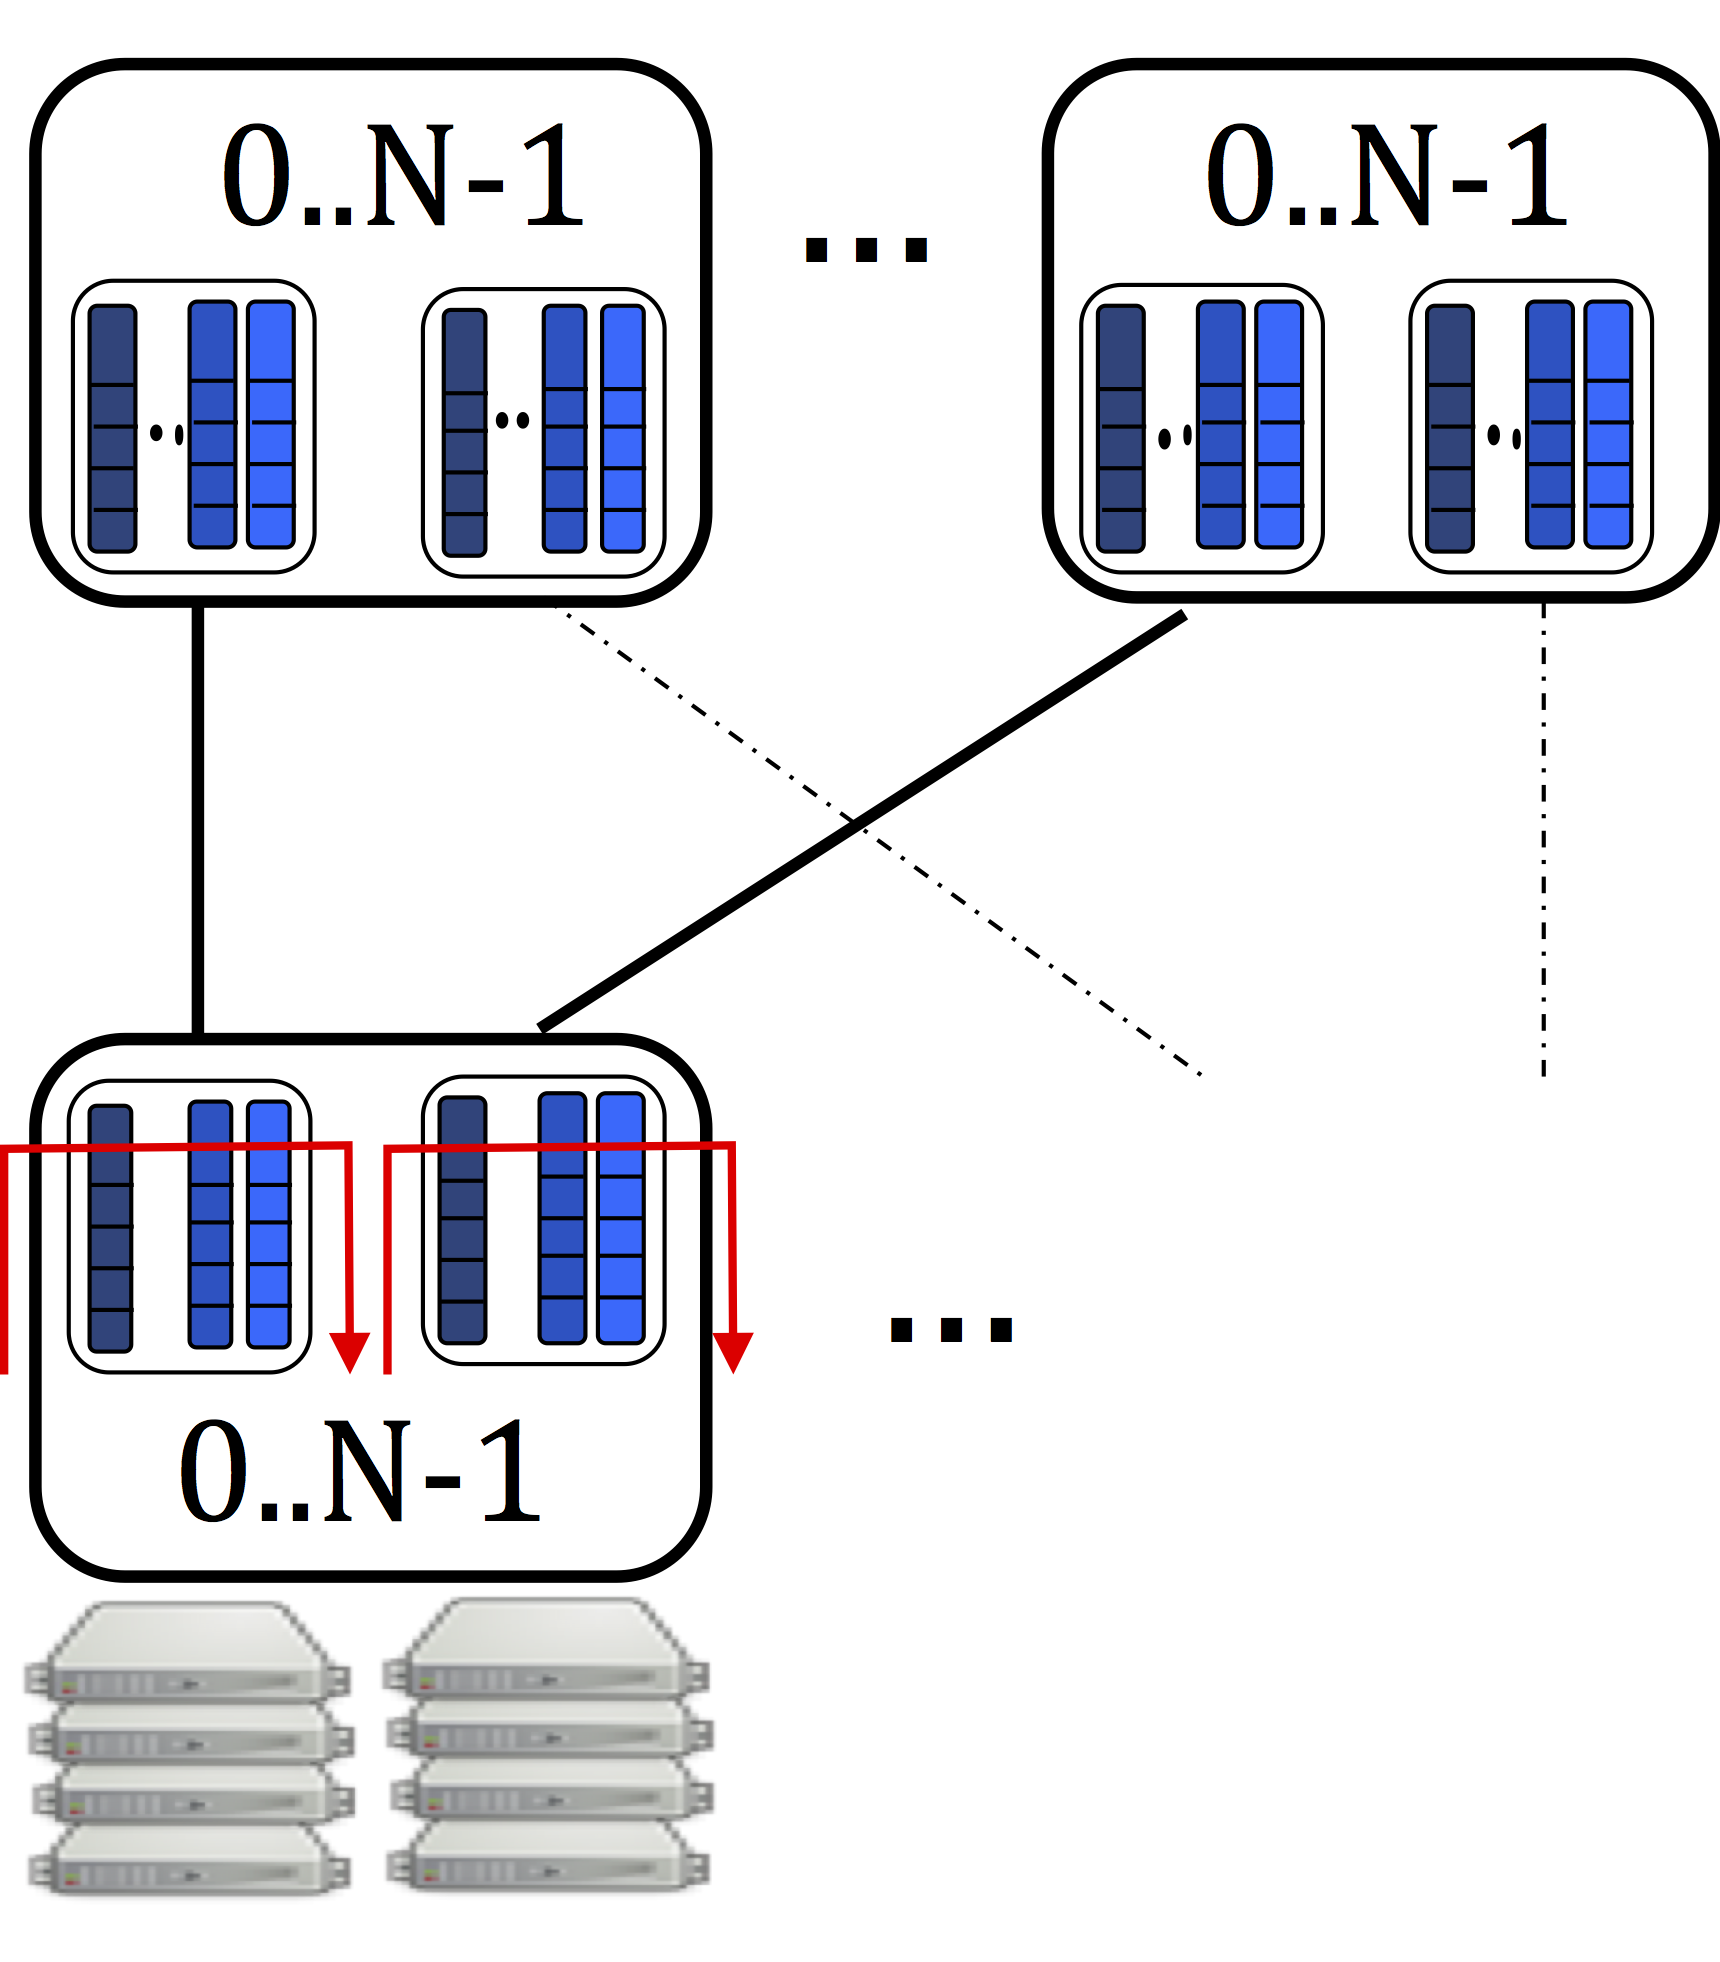
\includegraphics[width=\textwidth]{Chapter2/Figures/mlfq}
		\caption{MLFQ}
		\label{fig:sd-key-idea-mlfq}
	\end{subfigure}
	\hspace{0.2\textwidth}%
	\begin{subfigure}[htpb]{0.3\textwidth}
		\centering
		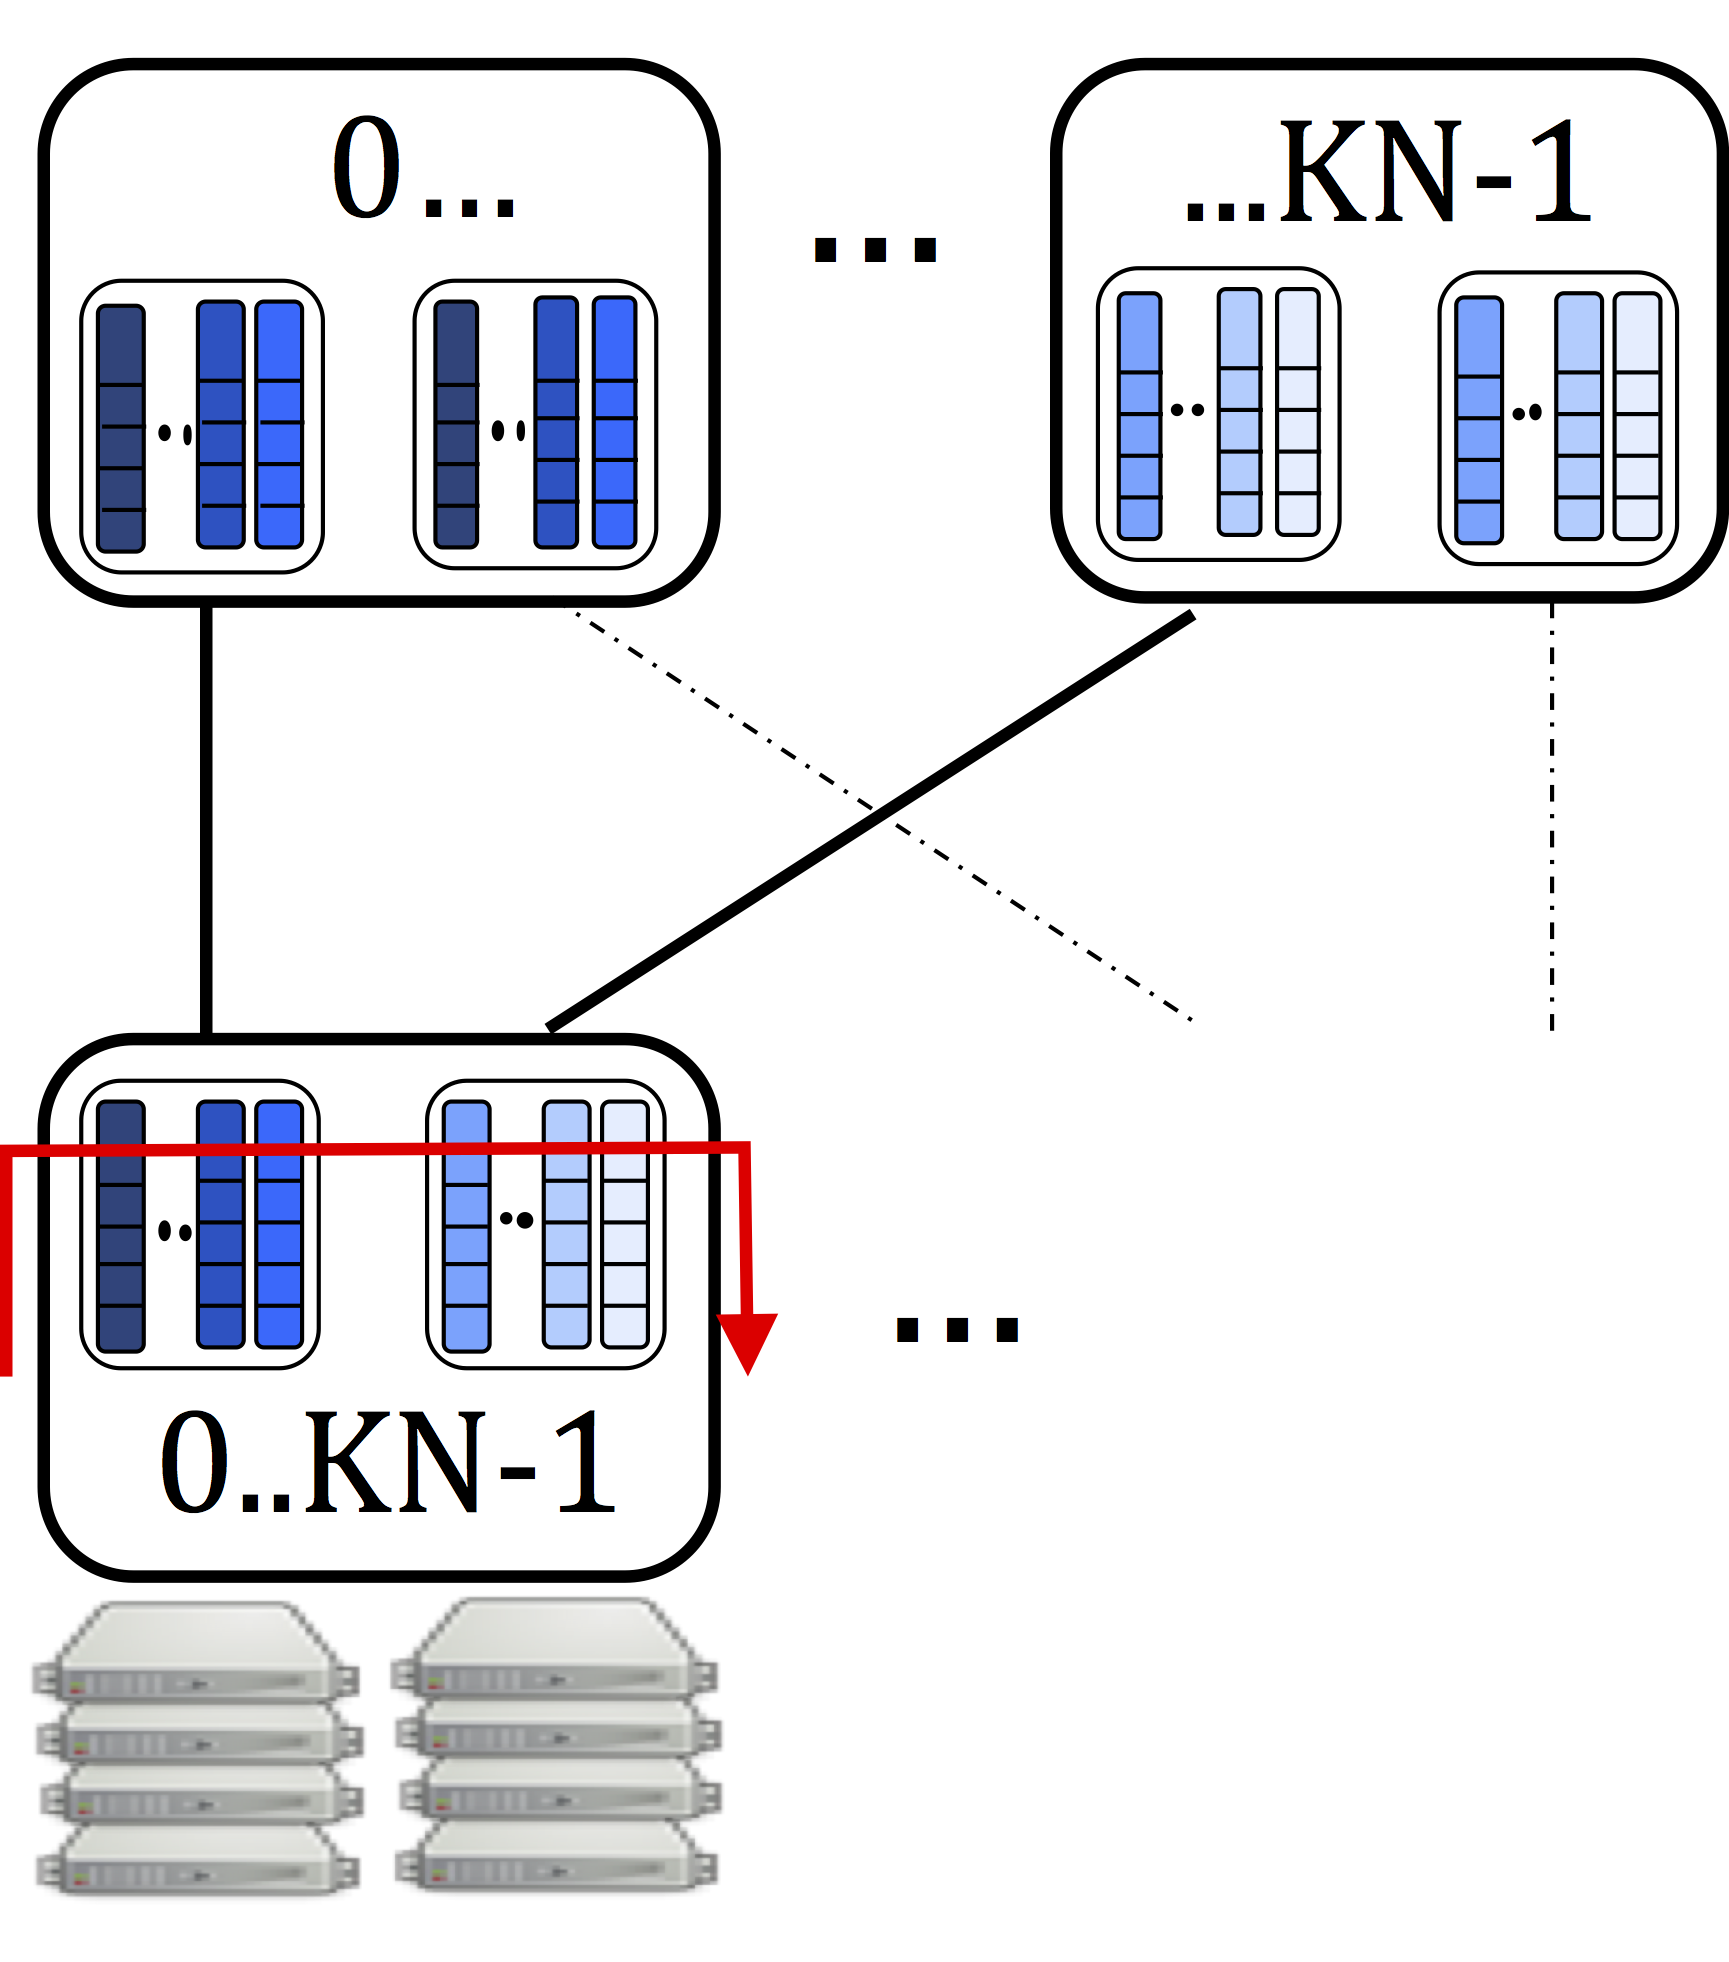
\includegraphics[width=\textwidth]{Chapter2/Figures/sdmlfq}
		\caption{SD-MLFQ}
		\label{fig:sd-key-idea-sdmlfq}
	\end{subfigure}
	\caption{Demotion extension with spatial diversity. Red arrows indicate demotion trajectory of the longest flow. On each switch is reported the priorities it handles. Lower indexes (and darker colors) correspond to higher priorities.}
	\label{fig:sd-key-idea}
\end{figure}
%Differently from 
The basic MLFQ (Fig.\ref{fig:sd-key-idea-mlfq}) focuses on the links individually and thanks to demotion moves flows, during their lifetime, across priority queues of single interfaces. Therefore, every interface handle the same priorities and flows are load balanced on different links independently from the prioritization mechanism. A standard technique for load balancing at flow-level is ECMP, which derives the next hop from the transport-layer tuple \texttt{\{IP ADDRESSES, PORTS, PROTOCOL ID\}}. Instead, our solution in Fig. \ref{fig:sd-key-idea-sdmlfq} --- which we call Spatially-Diverse MLFQ (SD-MLFQ) --- takes advantage of spatial diversity to extend the number of demotion levels beyond the limitation imposed by the PQs on a single interface. Interfaces from any ToR to the connected spines are virtually aggregated to offer a wider range of demotion levels. \\
One new aspect of this novel approach is that a demotion could imply shifting a flow from one path to another of equal-cost. In that light, the routing --- thus load balancing --- over the switching fabric is not blind to the prioritization machinery, but does depend on it. In general, a flow is moved both across queues and spines, effectively allowing a global resource exploitation for the demotion scheme. In order to have a clear and direct notation, the spines are labeled with the priorities handled by their interfaces. Notably, since the demotions that imply a spatial re-route take place at ToRs, all the interfaces on the same spine handle the same priorities. Hence, it is enough a single labeling per spine, valid for all its interfaces. 
A clear benefit of spatial diversity is that finer granularity in priorities is achieved even with few queues per port, at the price of a very limited implementation complexity. Also, elephant flows are better segregated from mice flows, as after a while they are physically moved to different paths inside the switching fabric. Despite its simplicity, relevant works exploring this solution in the field of data center networks seem to be lacking. 

\subsection{Queuing model}
\label{sec:threesystemcomparison}
%in the initial phase and get a first glance about its effectiveness
To tackle the spatial diversity framework from a conceptual perspective, three queuing systems are compared. They are shown in Fig.\ref{fig:three-system-comparison}. 
\begin{figure}
	\centering
	\begin{subfigure}[b]{0.3\textwidth}
		\centering
		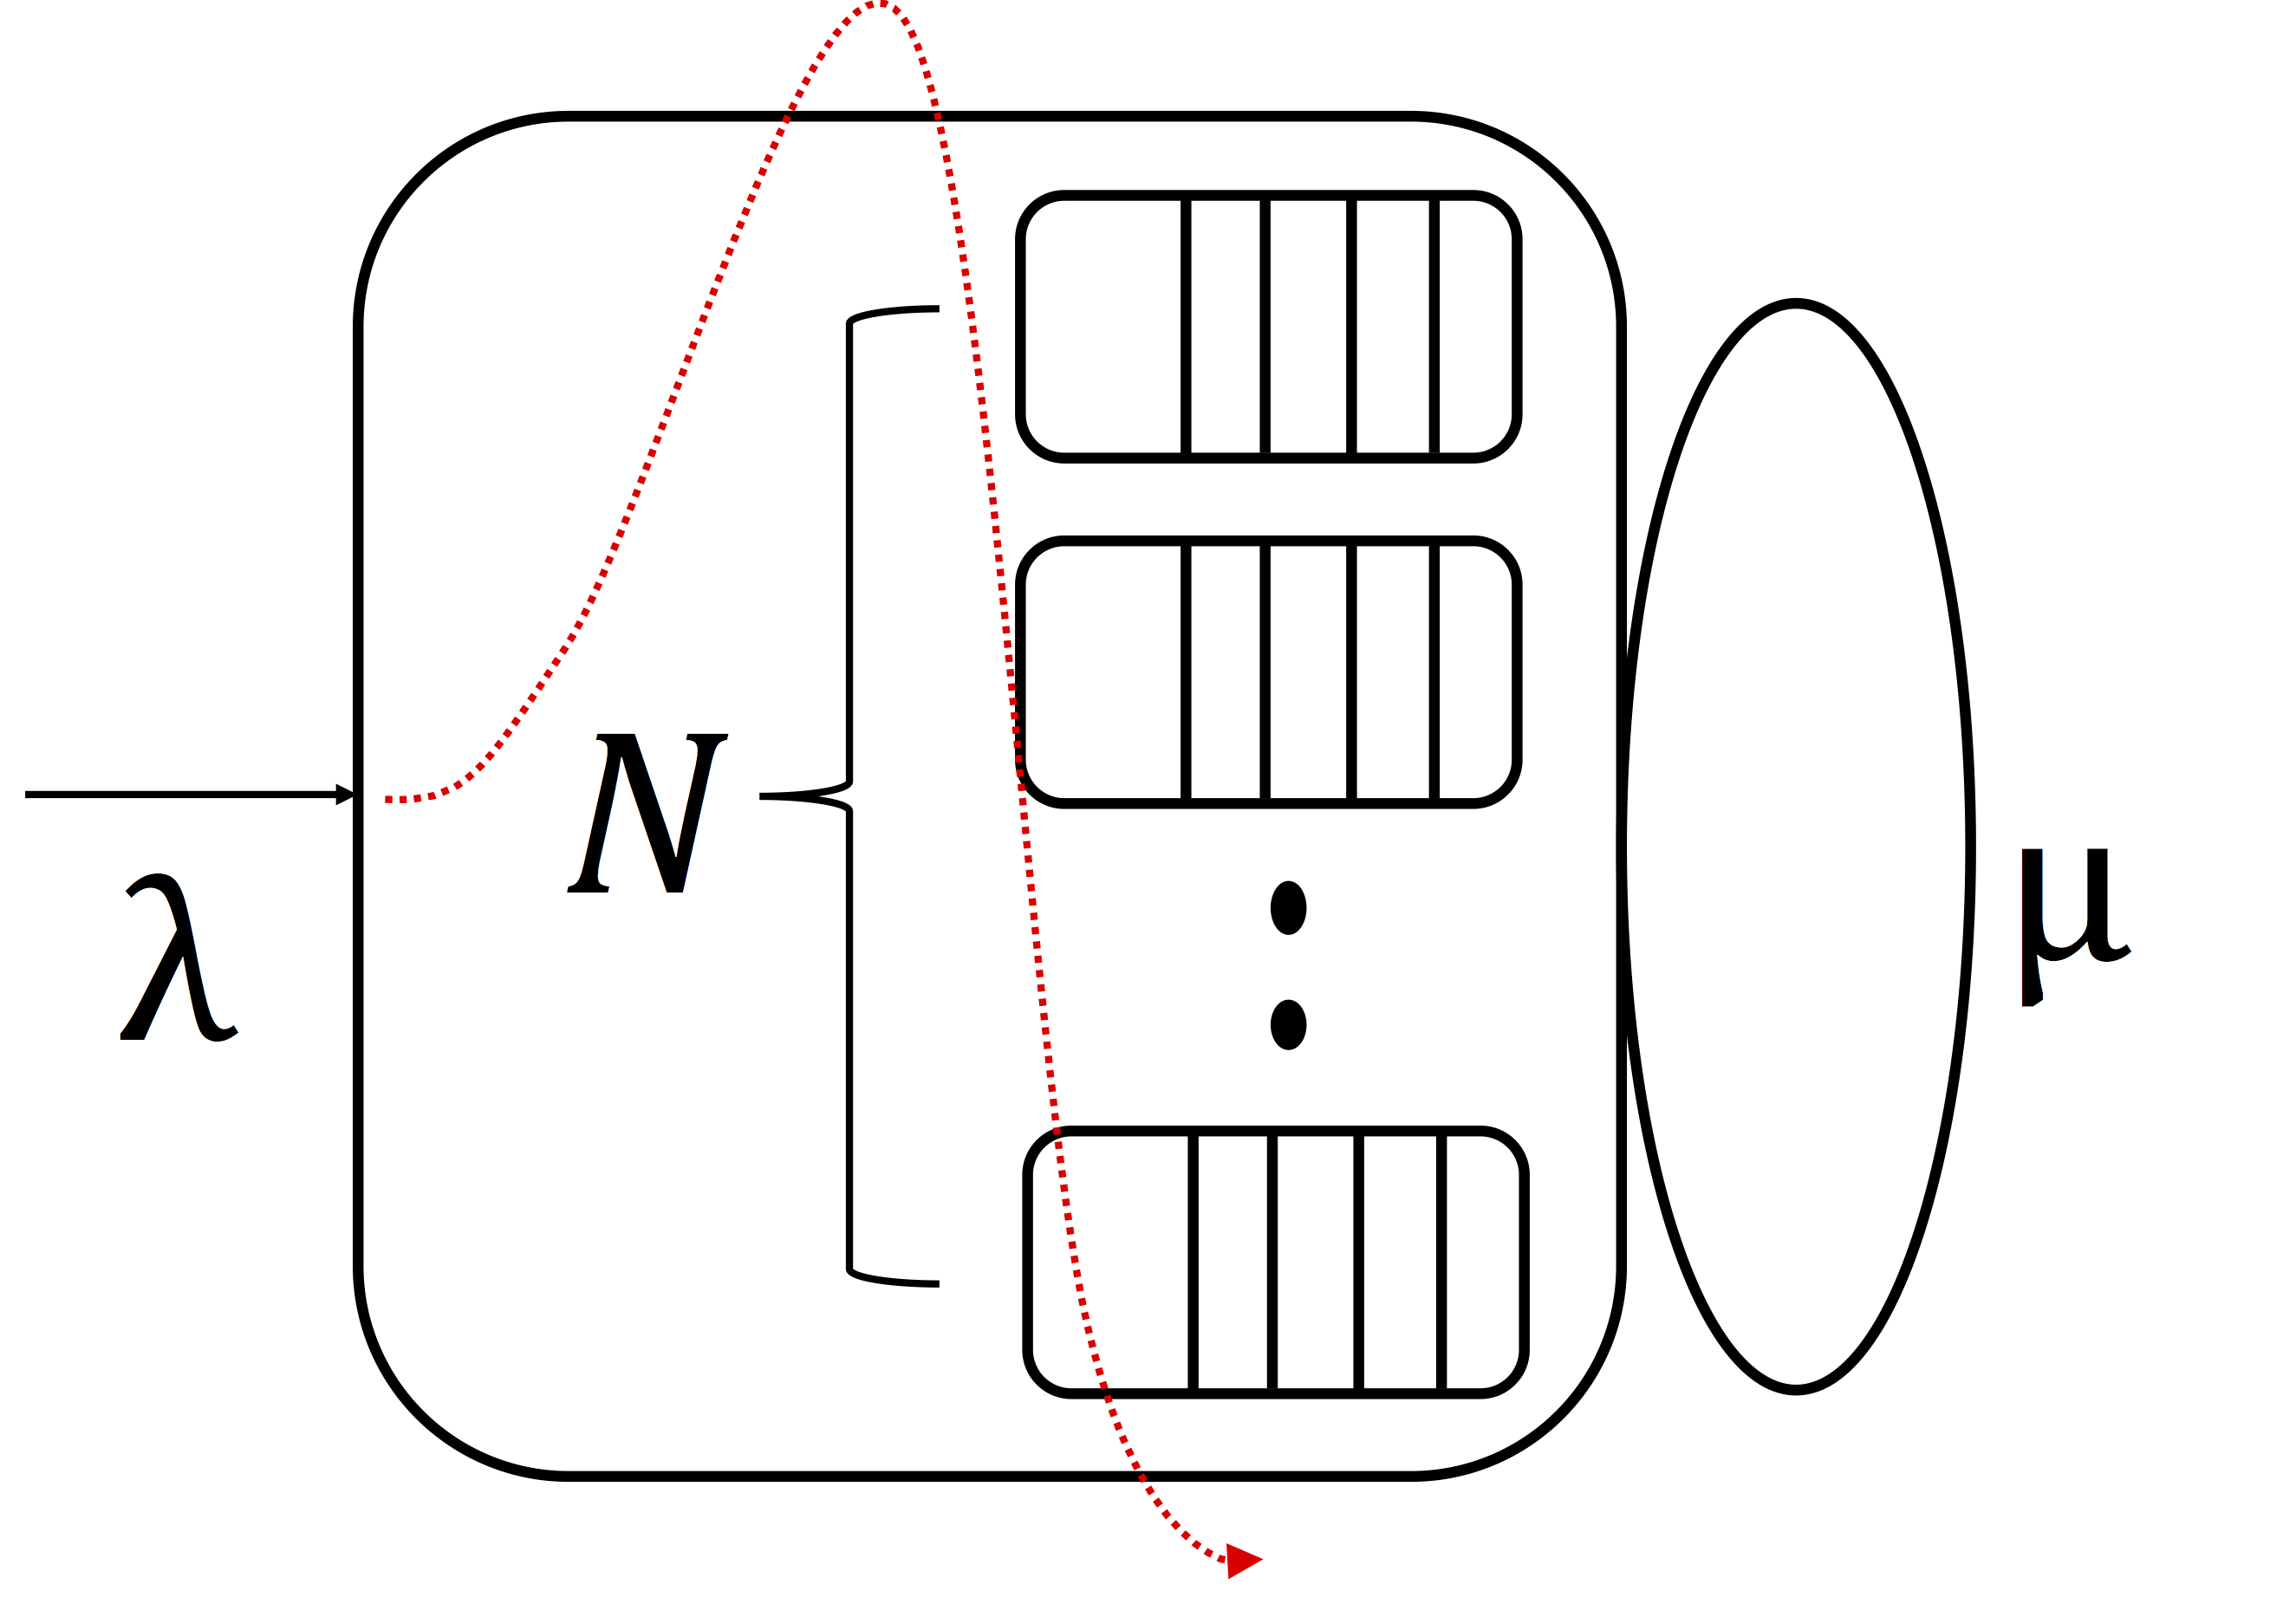
\includegraphics[width=\textwidth]{Chapter3/Figures/switchone}
		\smallskip
		\caption{Super-Server}
		\label{fig:switchone}
	\end{subfigure}
	\hfill
	\begin{subfigure}[b]{0.3\textwidth}
		\centering
		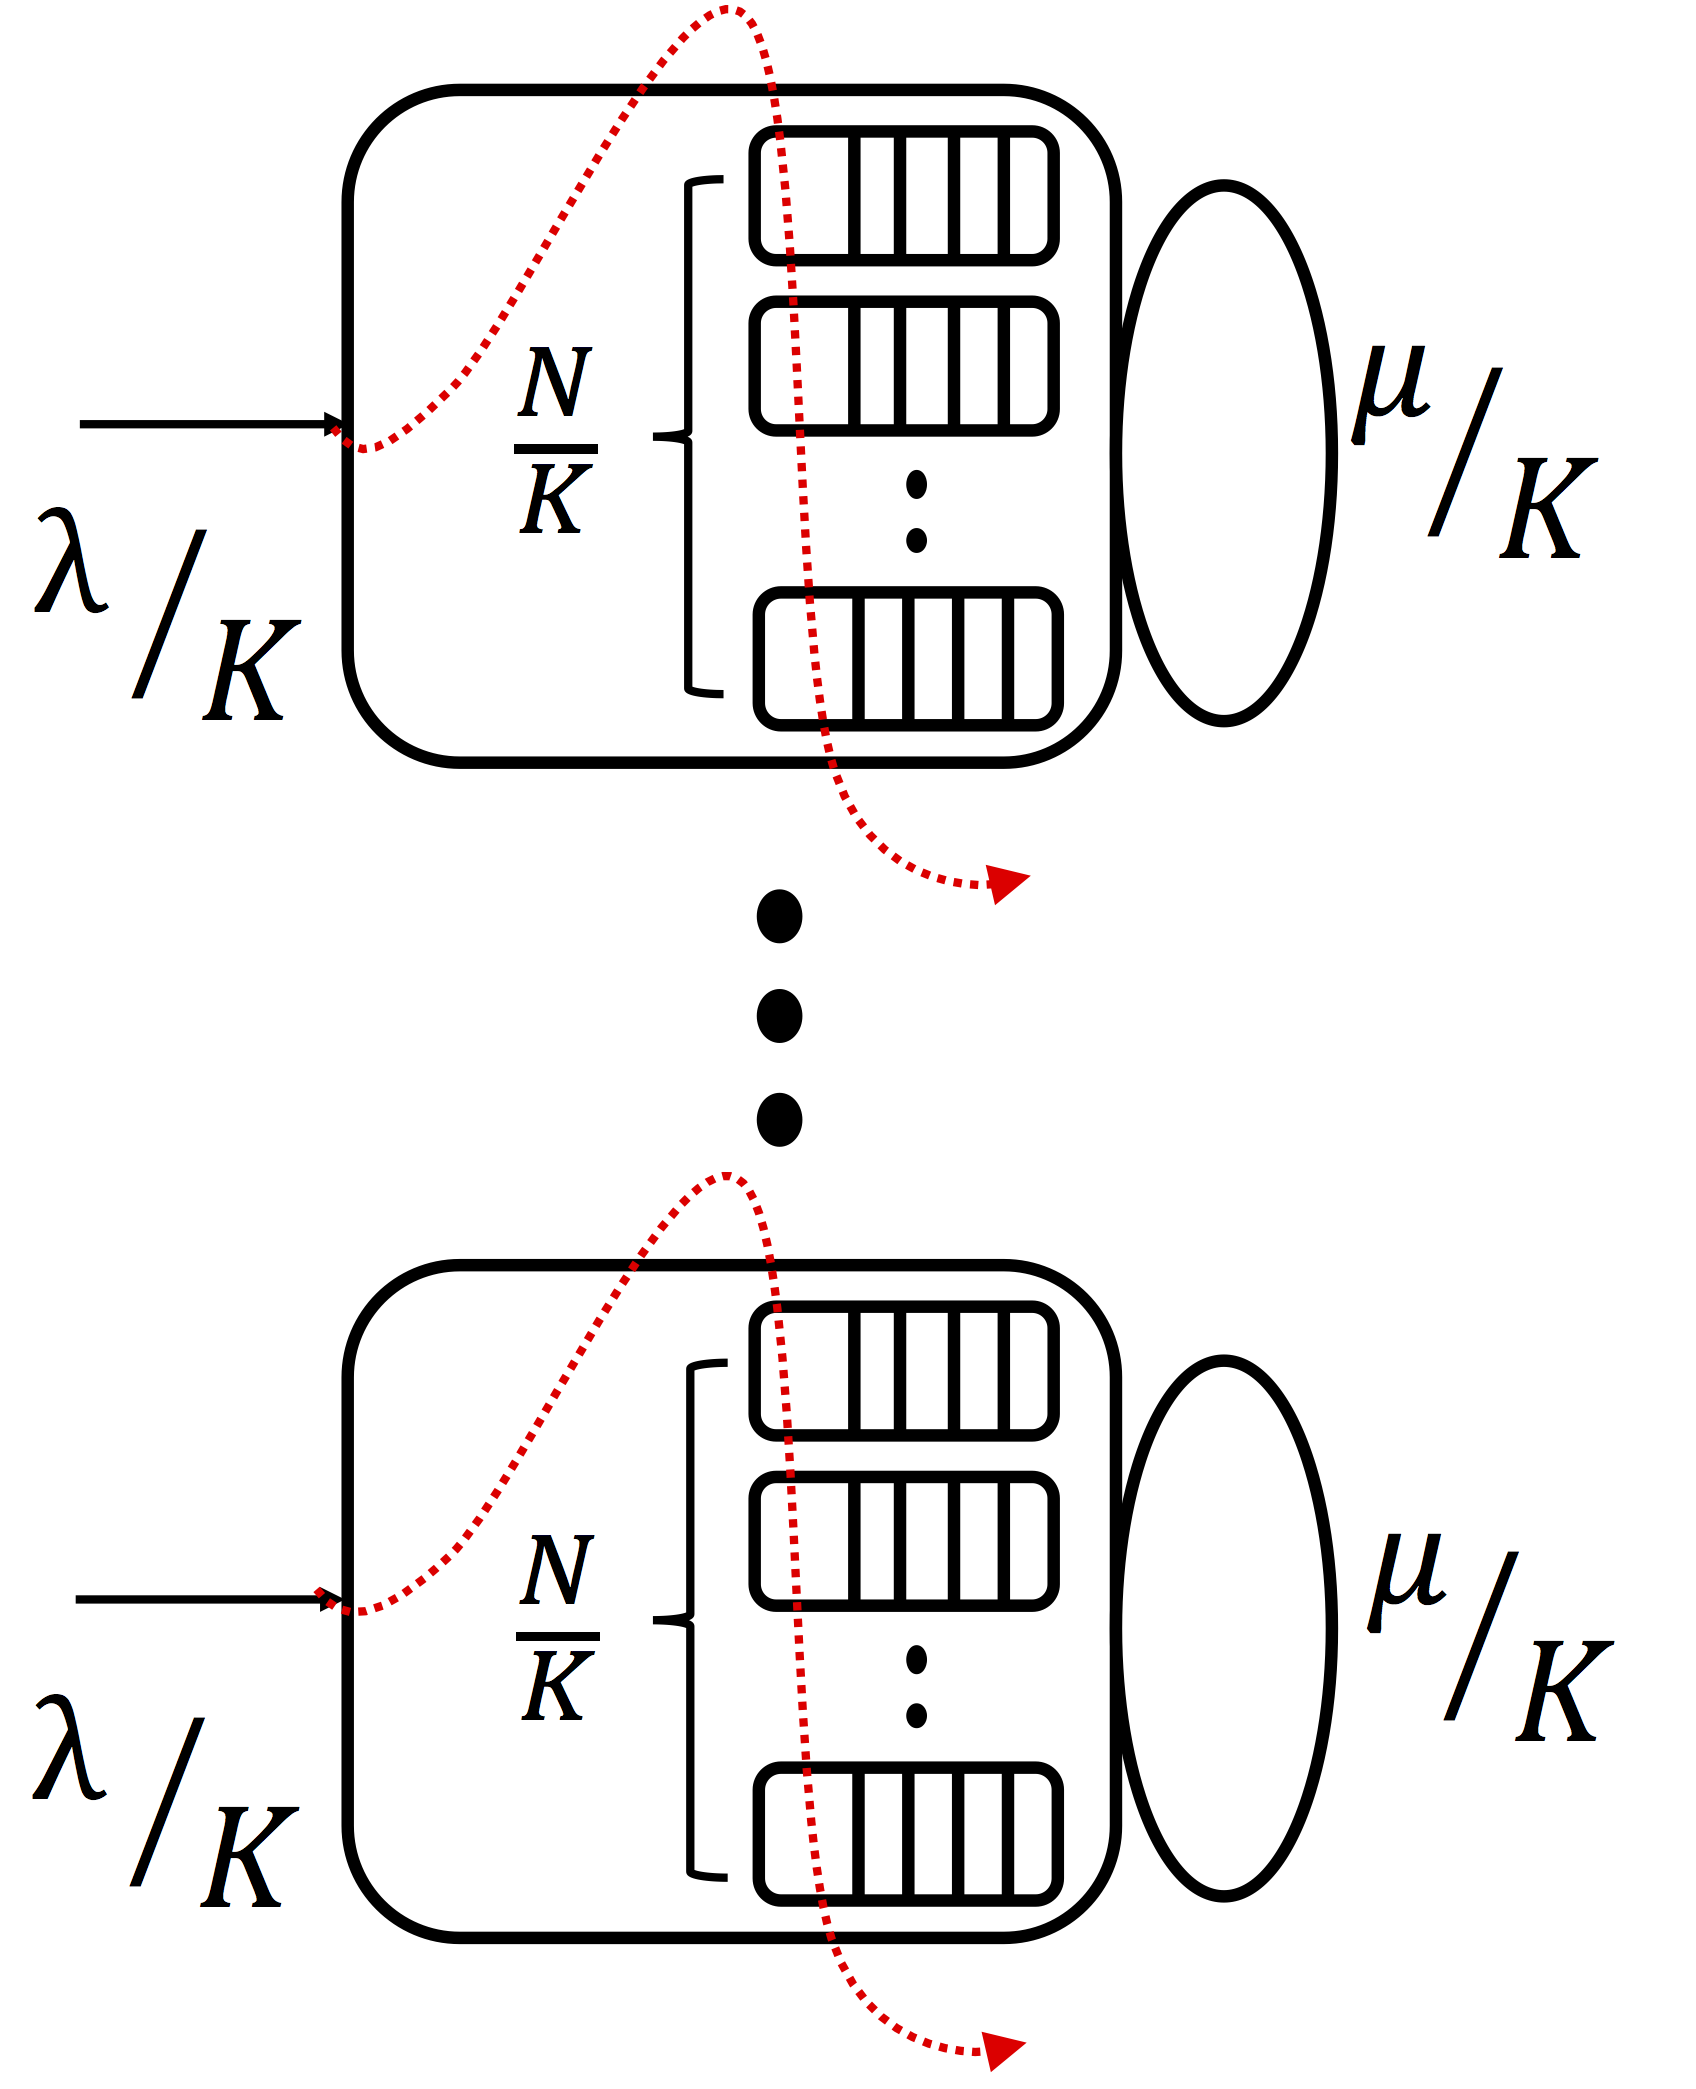
\includegraphics[width=0.8\textwidth]{Chapter3/Figures/esn}
		\caption{Independent servers}
		\label{fig:enn}
	\end{subfigure}
	\hfill
	\begin{subfigure}[b]{0.3\textwidth}
		\centering
		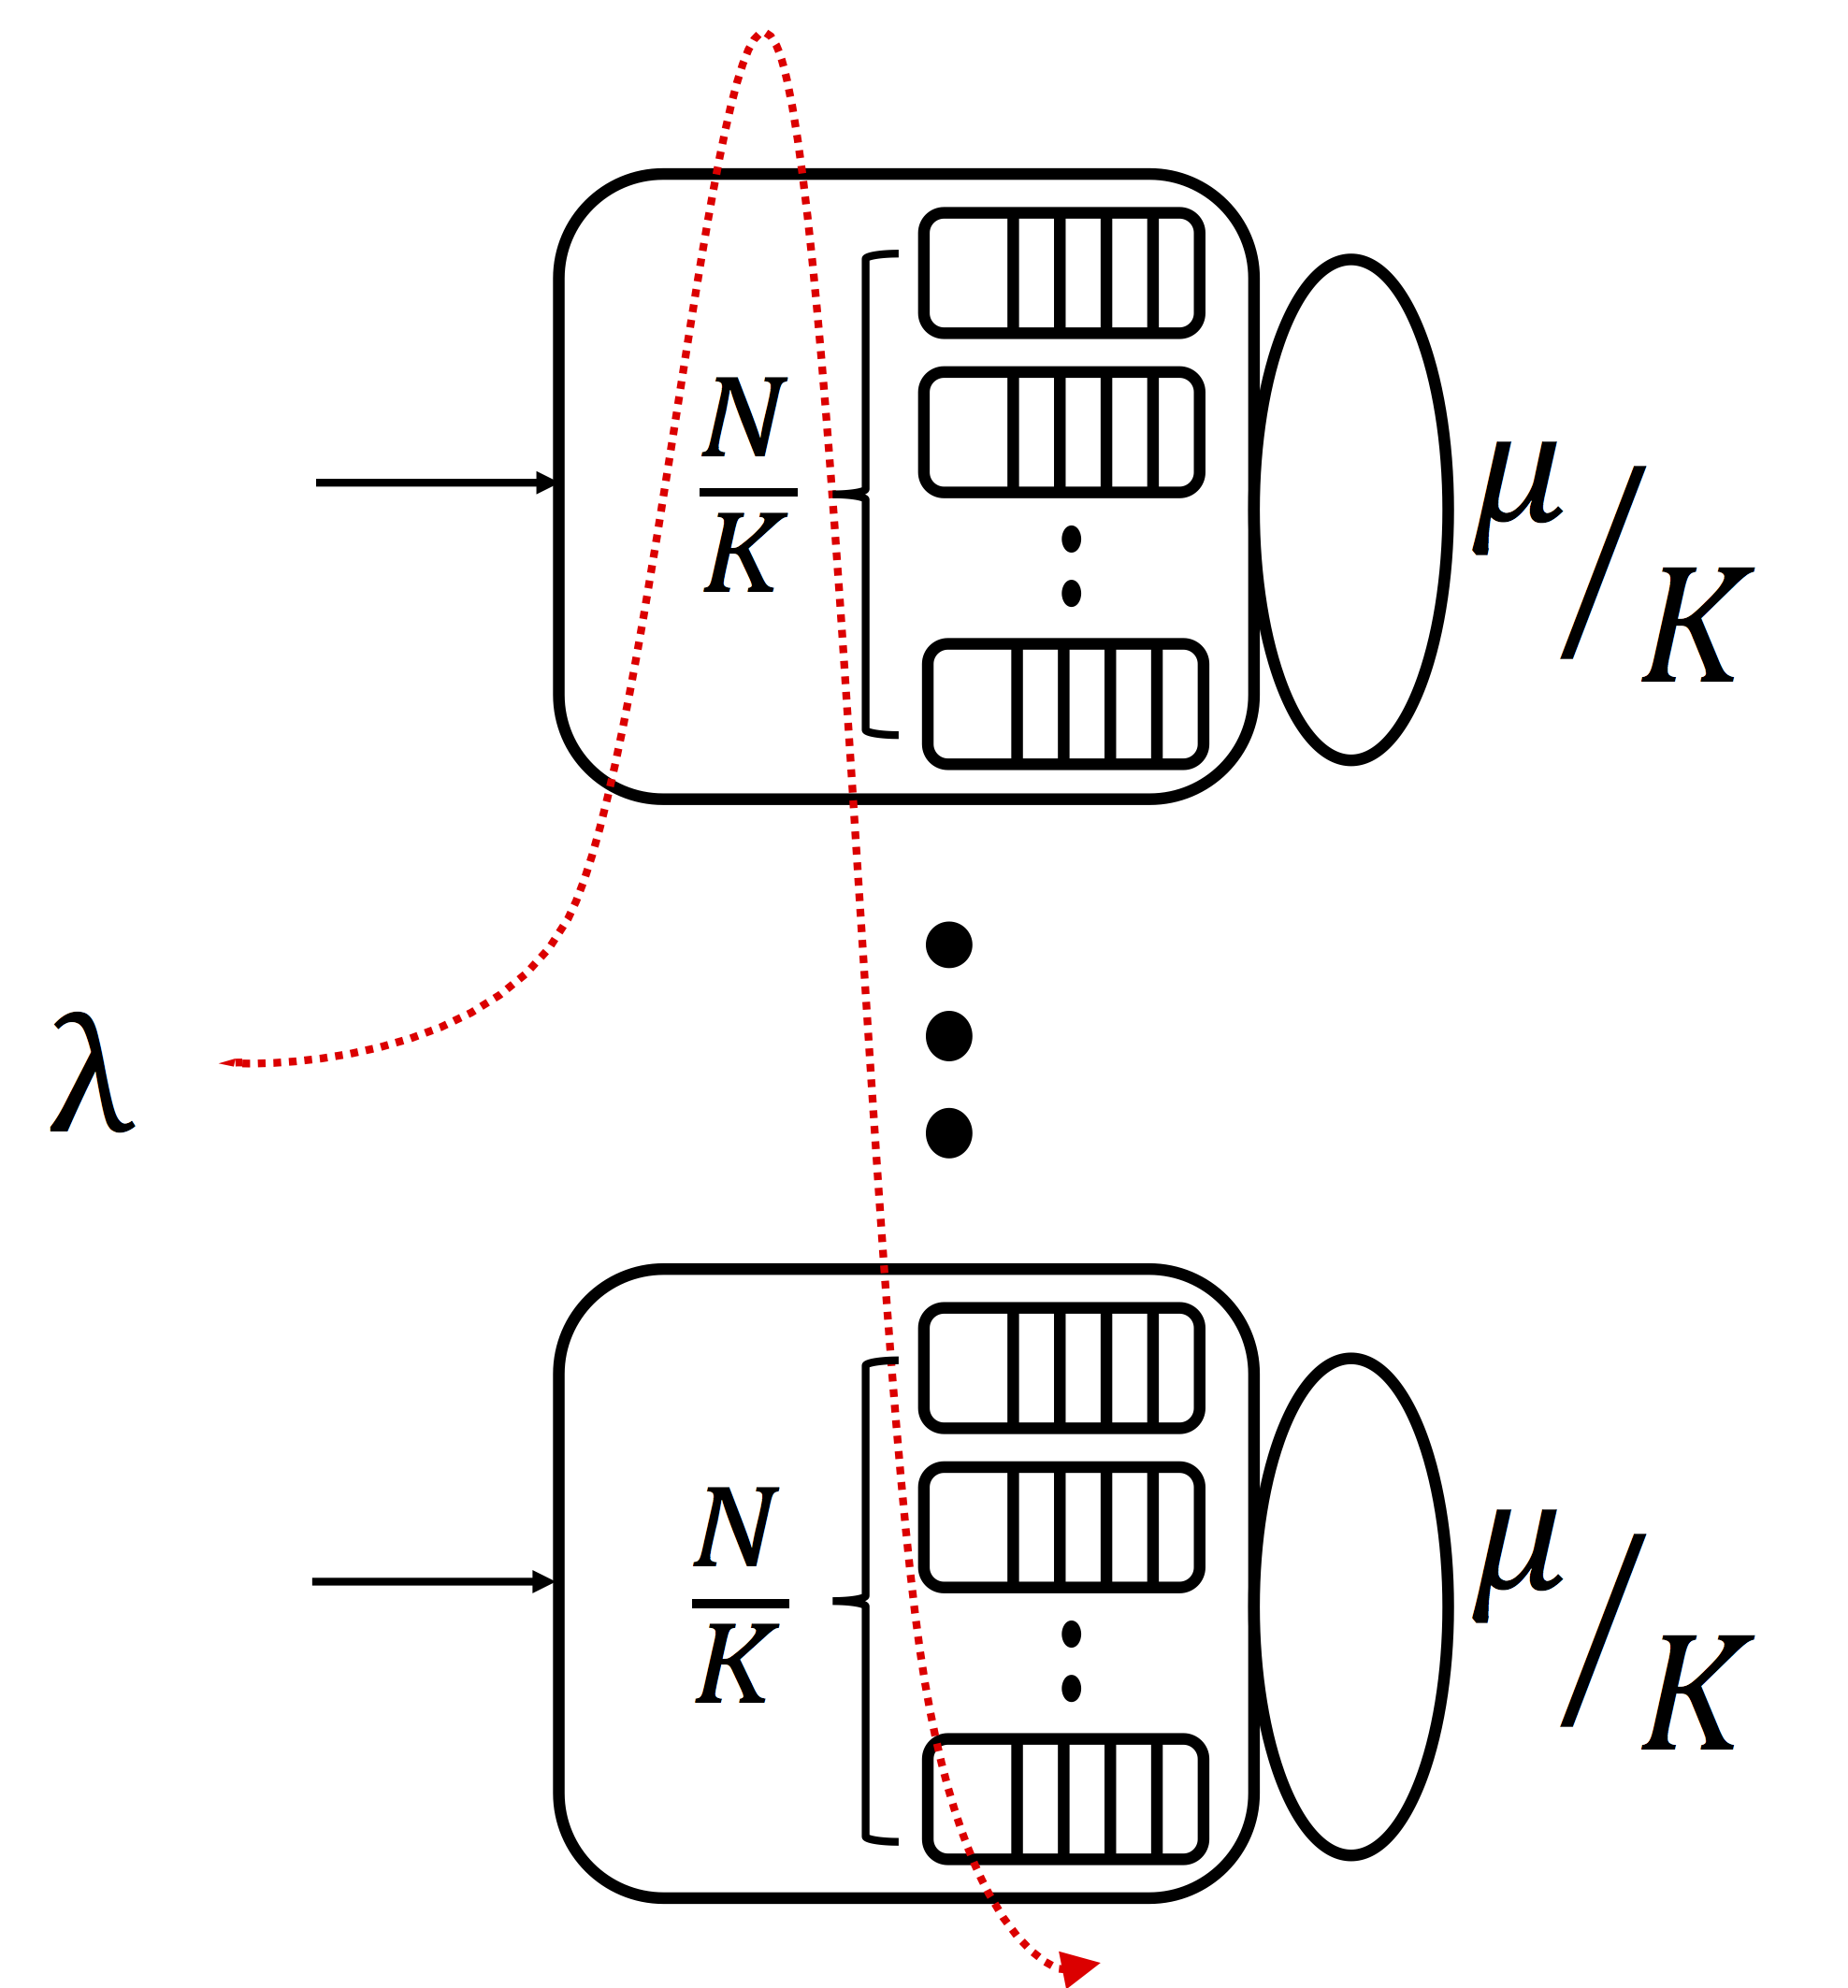
\includegraphics[width=0.9\textwidth]{Chapter3/Figures/sdmlfq}
		\caption{Spatial-diversity}
		\label{fig:sdmlfq}
	\end{subfigure}
	\caption{Three queuing system comparison.} %Red arrows indicate how queues are traversed during flow demotion. On each switch is reported the number of priorities it handles. Color scale is used to emphasize priority levels.}
	\label{fig:three-system-comparison}
\end{figure}
This is an abstraction of the real data center topology. At it heart, a Leaf-and-Spine network with $K$ spines can be described as a queuing system of $K$ parallel G/G/1 servers. Actually, these servers can be equivalently mapped to the \textit{up-send} interfaces that connects a ToR switch to all the spines, as well as to the \textit{down-send} interfaces from different spines to a single ToR. This mapping with the leaf-and-spine topology is shown in Figure \ref{fig:model-dc-map}, where the up-send interfaces are the ones with red texture, whereas the spine down-send interfaces are the ones with light green texture. Ingress and egress ports that connect end hosts to the datacenter network are ignored at this stage. This is in contrast with the data center abstraction provided by pFabric as a giant switch (Figure \ref{fig:pfabricdcn}), where the ingress and egress queues represented the bottleneck where to deploy scheduling strategies, whereas the switching fabric was assumed to be an ideal non-blocking interconnection. Somehow, differently from state-of-the-art solutions that focus only on the bottleneck links assuming that the network is able to sustain maximum throughput with negligible delays, the spatial-diversity approach shifts the attention to the queues inside the fabric itself and rethink the scheduling with a global DC view. Therefore, first it will be assessed the impact of spatial diversity with this simplified model which disregards the hosts and the ingress/egress interfaces, then we will proceed with the implementation on a simulated DCN afterwards.  \\
\begin{figure}
	\centering
	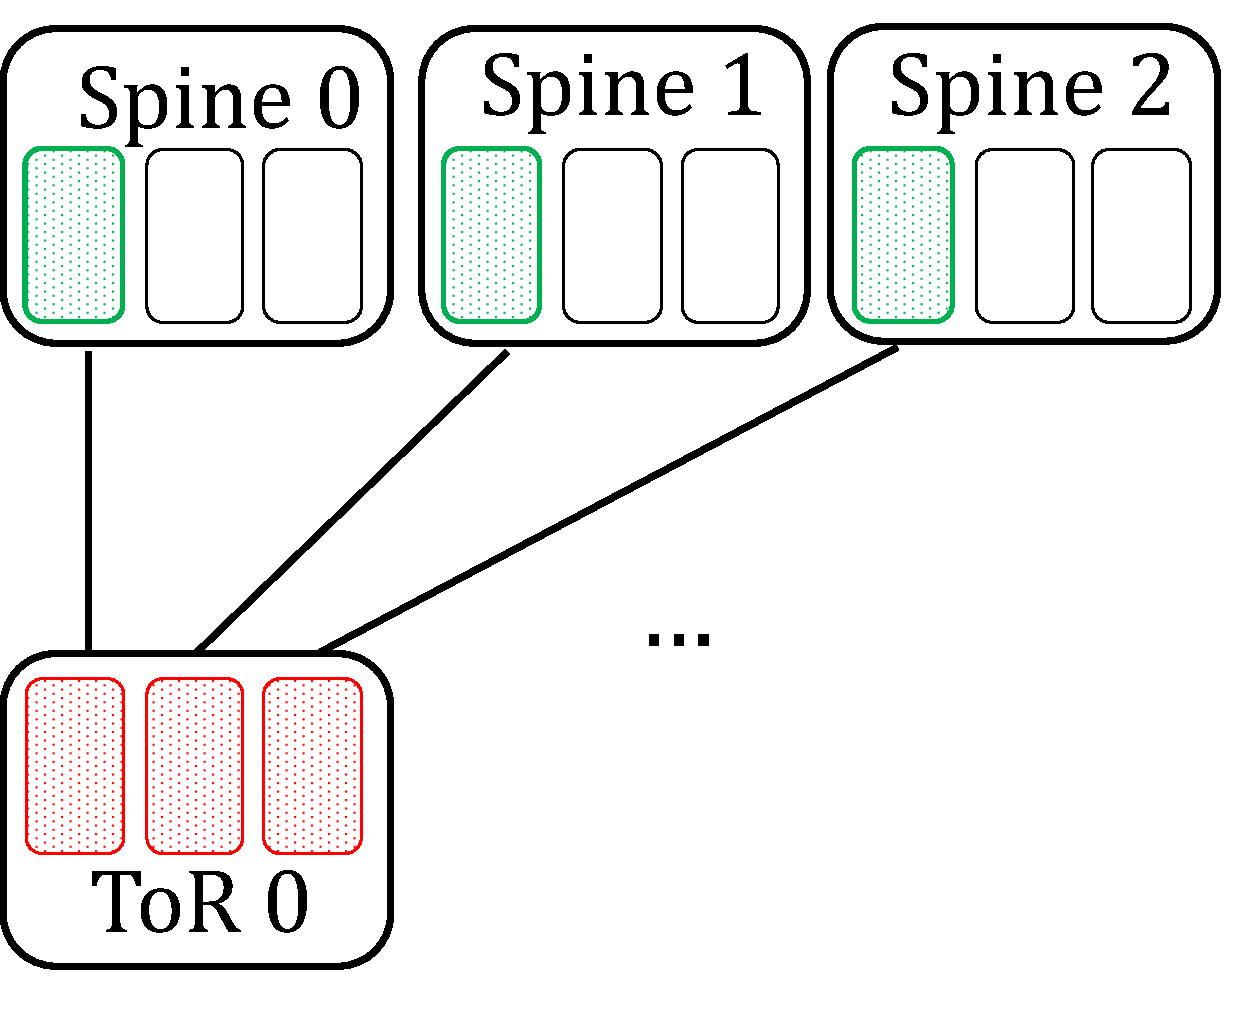
\includegraphics[width=0.3\textwidth]{ChapterSpatialDiversityFramework/Figures/model-dc-map}
	\caption{Mapping of the model abstraction with DCN topology}
	\label{fig:model-dc-map}
\end{figure}
From now on the interfaces considered in the abstract queuing model  of Figure \ref{fig:three-system-comparison} will be interchangeably referred to as servers or spines (with reference to the mapping with down-send spine interfaces).  

The three systems are different alternatives to handle the same total arrival rate $\lambda$ with the same total processing capability $\mu$ and the same number of priority demotion levels $N$. All systems use the mechanism of priority demotion first introduced by PIAS (\S \ref{sec:pias}). Instead, they differ in how priority levels are partitioned on a number $K$ of parallel servers and, more importantly, in the way they use available servers for flow demotion. Specifically, the longest flow that experience all possible demotions follows different trajectory across priority queues and servers. Flow trajectories are represented with dashed red arrows in Figure \ref{fig:three-system-comparison}\\
The first case (Fig. \ref{fig:switchone}) is to have a single high-capacity server that handles all priorities. This of course is the absolute best case where resources are fully concentrated, that provides the smallest delay but does not scale to the dimensions of real systems. It would be equivalent to realize an entire data center interconnection network with a single device of astonishing bandwidth. The second case (Fig. \ref{fig:enn}) is the legacy way to handle priority demotion, where all servers are treated independently in parallel. Flows are evenly load balanced on the available servers and moved across priorities of the same server during their lifetime. In this case the number of demotion levels are limited to \small$\frac{N}{K}$\normalsize. Finally, the third case (Fig. \ref{fig:sdmlfq}) is the novel object we want to investigate, where all the flows are initially sent to the same server, then demoted on the $N$ globally available priority queues. In this case subsequent servers are configured to handle lower and lower priorities, thus part of the flows are re-routed as a consequence of the spatial-diversity. For this reason, in the following of this work also the servers and the links will be labeled as "high priority" or "low priority" for brevity, meaning that they handle high priority traffic or low priority traffic, respectively. 

It was already defined a rigorous mathematical formulation for representing the demotion across priority queues in a single servers as a tandem of M/M/1 queues. (\S. \ref{sec:pias-queueing-model}). The system with spatial diversity introduces a new set of thresholds, which mark the amount of service after which a flow is rerouted to another server. The next section presents a complete formulation for modeling spatial-diversity, starting from the model already defined. 
\section{Mathematical formulation}
\label{sec:complete-model}
The introduction of spatial diversity adds a level of complexity to the system. Let's formalize the system setup. There are $K$ parallel servers with $N$ priority queues each one. Thus, there are a total of $K \times N$ priority queues.  All of them are used to add new levels for demotion, therefore flows can assume priority $p \in [1,KN]$ with no duplicate priorities and there are $K \times N - 1$ demotion thresholds. Let's use the variable $j \in [1,K]$ to index the servers and the variable $i \in [1,N]$ to index the priority queues inside each server $s_j$. Starting from the highest level of priority $p$=1 and following descending order of priority up to $p=KN$, the priority levels are assigned to servers from the lower index to the higher index. Thus, server $s_1$ handle priorities $p=\{1,..,N\}$, server $s_2$ handle $p=\{N+1,..,2N\}$, and so on. As in the MLFQ system, whenever a flow at priority $p$ has received service equal to the next threshold, it is downgraded at priority $p+1$. However, differently from MLFQ, it may happen that priority $p$ is assigned to server $s_j$, while $p+1$ is handled by server $s_{j+1}$. In such a case, the flow must be rerouted to a different server. Thus, two related problems need to be solved: finding the set of thresholds that triggers a new flow route from server $s_j$ to server $s_{j+1}$, and finding for each server $s_j$ the set of thresholds that mark the demotion from PQ $i$ to PQ $i+1$, when both PQs are in server $s$. Let's denote them as \emph{load-balance thresholds} and \emph{sub-thresholds}, respectively. 
\smallskip
\begin{tcolorbox}[title=Terminology]
	In a system with priority demotion and with spatial diversity, a flow is moved to a different priority queue (PQ) when the service it has obtained is larger than some threshold. We say that the threshold \textit{push} a flow to a new PQ. We recognize two set of thresholds:
	\begin{itemize}
		\item \textbf{\emph{Load balance thresholds}}. The set of demotion thresholds that push a flow in a priority queue on a server different from the server currently handling the flow itself, implying a flow rerouting.
		\item \textbf{\emph{Sub-thresholds}}. The set of thresholds that push a flow in a different priority queue but in the same server as the one currently handling the flow itself. 
	\end{itemize}
	Correspondingly, we will refer to as:
	\begin{itemize}
		\item \textbf{\emph{Inter-server[spine] demotion.}} A priority demotion involving a load balance threshold.
		\item \textbf{\emph{Intra-server[spine] demotion.}} A priority demotion involving a sub-threshold.
	\end{itemize}
\end{tcolorbox}
\smallskip
The name \emph{load-balance} derive from the fact that the values of these thresholds have strong implications on how the load is distributed across servers. If the thresholds are too small, flows are early rerouted on low priority paths and the capacity of high priority links is essentially wasted. For a real data center implementation this would mean a reduction in the maximum throughput sustained by the switching fabric. As a trivial example, consider a simple topology with two parallel servers each one of normalized capacity 1. In this topology there is only a single threshold that may trigger a flow reroute. With an ideal load balance that evenly distributes the traffic among the two servers, this topology offers a maximum normalized throughput of 2. However, an inappropriate setting of the aforementioned demotion threshold that immediately reroutes flows after negligible attained service would in practice reduce the total capacity  of 50\%. On the other end, still this threshold could be optimal if considering only micro flows, whereas the equal load balance which uniformly splits the traffic on available servers may correspond to a bad demotion threshold for the FCT minimization. In short, a careful tuning of load balance is a new trade-off that was nonexistent in the legacy MLFQ framework, where traffic was demoted to different priority queues but always in the same interface (i.e. link), with zero effects on load balancing. Indeed, a threshold setting that gives an unbalanced load allocation in the available priority queues affects only the delays but not the maximum throughput that the network can sustain. \\
%In SD-MLFQ, depending on the shape of the flow size distribution, latency constrained traffic would either remain unnecessarily mixed with non-demanding latency flows or immediately get.
As concerns the sub-thresholds, they push flows to the same kind of intra-server demotion already studied for MLFQ. However, MLFQ servers work independently and in parallel (Fig. \ref{fig:sd-key-idea-mlfq}) and they are all fed with the same job size distribution. Instead, SD-MLFQ servers observe a different version of the initial workload. Indeed, subsequent servers receive only flows larger than the precedent demotion thresholds, thus they handle truncations of the original flow size distribution above increasing percentiles. As a consequence, while MLFQ thresholds are computed once for all servers, SD-MLFQ sub-thresholds should be optimized depending on the server they belong to. A clarifying overview is provided in Fig. \ref{fig:sd-spine-distribution} for the case of $K$=3 servers $s_1,s_2,s_3$. Figure \ref{fig:wsbp-cdf} is an example job size distribution, from which new flows are randomly generated. In a data center network, this would be the DC-wide workload. On the same axes are drawn the two example split thresholds, denoting the amount of service in kilobytes after which a flow is rerouted from $s_1$ to $s_2$ and then from $s_2$ to $s_3$. 
\begin{figure}
	\centering
	\captionsetup{width=.8\linewidth}
	\begin{subfigure}{.3\textwidth}
		\centering
		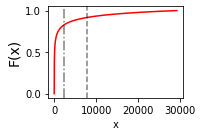
\includegraphics[width=1.05\textwidth]{Chapter3/Figures/ws-bp-cdf}
		\caption{Workload on $s_1$}
		\label{fig:wsbp-cdf}
	\end{subfigure}%
	\hfill
	\begin{subfigure}{.3\textwidth}
		\centering
		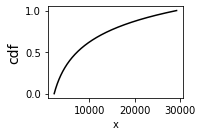
\includegraphics[width=\textwidth]{Chapter3/Figures/wsbp-highp-cdf}
		\caption{Workload on $s_2$}
		\label{fig:highp-cdf}
	\end{subfigure}
	\hfill
	\begin{subfigure}{.3\textwidth}
		\centering
		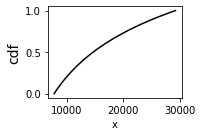
\includegraphics[width=\textwidth]{Chapter3/Figures/wsbp-lowp-cdf}
		\caption{Workload on $s_3$}
		\label{fig:lowp-cdf}
	\end{subfigure}
	\caption{Job size distributions observed by servers $s_1$, $s_2$, $s_3$ in decreasing order of priority. Optimal load balance split for $\lambda=0.9$.}
	\label{fig:sd-spine-distribution}
\end{figure}
Since all flows enter the system through $s_1$, this distribution is also the one observed by the highest priority server $s_1$. Then, subsequent servers of lower priorities observe left-truncated versions of the initial workload on $s_1$. 


An intuitive solution to address both load balance thresholds and sub-thresholds at once is to write an extension to the PIAS model that embeds spatial-diversity. This formulation, explained in details below, would in principle guarantee optimal performances. Indeed, it jointly captures in a unique model all the dynamics of the system.
\subsubsection{Optimal solution}
The optimization problem Eq.\eqref{eq::costfunction} can be extended to the case of spatial diversity.
Assume the capacity of a single server to be $\mu/K$, so that the total capacity is always $\mu$. All the servers work independently with same rate $\mu / K$. Still there is a SP scheduler orchestrating priority queues in every server, but there is no coordination among different servers, meaning that there is not a global SP scheduler to discipline the transmission among distinct servers. Indeed, such a tight control among physically different devices would be almost impossible to realize in practice, at least packet by packet. \\
Let the notation $\mu_i^j$ indicate the drain rate of the $i$-th queue in the $j$-th server $s_j$ $(1 \le i \le N, 1 \le j \le K)$, and equivalently use $\lambda_i^j$ for the arrival intensities and in general the superscript $j$ for any quantity already defined for the queues in the basic model in Sec.\ref{sec:pias-queueing-model} but applied to queues inside server $s_j$. A summary of all the quantities involved in the queuing model is found in Table $\ref{tab:queuingmodel}$. It follows:
\begin{align*}
\lambda_i^j &= \lambda \mathbb{E}[L_i^j] \\
\mu_i^j &=  \dfrac{\mu}{K} \prod_{l=1}^{i-1}(1-\rho_l^j) \\
\theta_i^j &= F(\alpha_i^j) - F(\alpha_{i-1}^j)	\\
\mathbb{E}[T_i^j] &= \dfrac{1}{\mu_i^j - \lambda_i^j}
\end{align*}
The formulation is essentially the same but with an additional dimension that takes into account the existence of multiple servers. Every server is modeled as a tandem of $N$ queues, exactly as in PIAS. Then, there are $K$ of them in parallel. Also, we wrote an additional constraint Eq.\eqref{eq:overload-constr} that prevents overloading any spine.
\begin{subequations}
	\begin{align}
	&\underset{\{\theta_i^j\}}{\text{min}} & \quad  & \mathcal{T} =	\sum_{j=1}^{K}\sum_{i=1}^{N} \theta_i^j \sum_{j=i}^{N}T^s_j 					\label{eq::costfunction-spatial} & \\
	&\text{subject to} & \quad  &\theta_i^s \ge 0 & \\
	& & & \sum_{i=1}^{N} \theta_i^j = 1  \qquad \forall j \in [1,K] &  \\
	& & & \sum_{i=1}^{N}  \lambda_i^j < \mu/K  \qquad \forall j \in [1,K] & \label{eq:overload-constr}
	\end{align}
\end{subequations}
This approach would provide optimal load balancing and at the same time would choose a set of sub-thresholds targeted on the optimal load balance thresholds. Notably, the optimal solution would never include load balance thresholds that lead to an unbalanced traffic distribution among the servers, because that would have an overkilling effect on the delays, which instead the problem tries to minimize. Despite being a clean analytical formulation, its complexity seems prohibitive. The basic model without spatial diversity yet was non-convex and presented products and ratios of variables (Sec. \ref{sec:pias-queueing-model}). Nonetheless, it is still tractable since the number of variables is typically bounded to the (low) number of PQs available in commodity switches. Instead, in the complete model the number of variables scales with the product $K \times N$, where $K$ is usually big for large-scale data centers. In the next chapter we will provide in more details the CPU-time spent by two well-known meta-heuristics solvers, specifically PSO \cite{pso,pso2} and Basin-Hoppin \cite{basinhoppin} before to converge. Anyway, if the time scale at which a solution could be found is excessively large, the system would be unable to react promptly to a sudden change of the flow size distribution. As a consequence, the system would operate for long using thresholds mismatched with respect to the flow distribution. Therefore, even finding an optimal solution once does not signify that this approach is feasible for a real datacenter scenario, where likely the solution must be computed repeatedly as statistics change. \\
To the purpose of investigating the spatial diversity framework, it has been preferred to handle the two problems individually. The approach that has been carried out is decoupled in two sequential steps.
\begin{enumerate}
	\item \textbf{Optimize load-balance thresholds.} First it is solved an optimization problem with the goal of finding the best load partitioning among $K$ servers. Servers are always assumed to have a single priority ($N$=1), because for the time being sub-thresholds are ignored. At the end of this phase a set of $K$-1 load balance thresholds is delivered.
	\item \textbf{Greedy subthresholds}. The load-balance thresholds are provided as input of the second phase. They split the support of the flow size in $K$ disjoint intervals covering the whole support. The $i$-th interval contains the sizes of those flows that end their service in server of priority $i$. On each interval is computed a set of sub-thresholds with a greedy algorithm like ES-N or LS-N, but applied to the truncated distributions (Sec.\ref{sec:greedy-thresh}).  
	%Each of them truncates the original flow size distribution at a given percentile. 
\end{enumerate}

\subsection{Traffic load balancing}
\label{sec:decoupling}
\subsubsection{Optimize load balance thresholds}
\label{sec:optimal-lb-problem}
For the first phase turns out again to be useful the stochastic queuing model of MLFQ as provided in PIAS. (Sec.\ref{sec:pias-queueing-model}-Fig.\ref{fig:pias_scheme}). Each server is equipped with a single priority queue per port, therefore the optimal load balance problem can be abstracted with exactly the same model, where each queue in the tandem maps a server. After all, in this case priority queues are physically distributed to different servers, instead of being part of the same interface. They are independent on each other and the strict priority scheduler is no more involved, as they work in parallel without coordination. Practically, the only modification is to the queues capacities $\mu_i$. Remember that in the aforementioned MLFQ model the strict priority scheduler was described by attenuating the PQ serving rates $\mu_i = \mu\prod_{i}(1-\rho_i)$ for increasing $i$. Because of servers work in parallel without scheduling, this expression is not needed anymore and the draining rates just coincide to the same value:
\[
\mu_i = \mu \mslash K, \qquad i=1,..,K
\]
% TODO Keep in mind that these are just the flow size distributions and not the actual traffic handled by a server. For example, $s_0$ serve only the first $\Omega_1$ bytes of all flows, including those larger than $\Omega_1$ . The actual byte arrivals were obtained with Eq.\eqref{load-on-pqi}, that does require these distributions to be known.
\subsubsection{Choose greedy sub-thresholds}
\label{sec:subthresh-with-sd}
Lastly, it is addressed the problem of finding the sub-thresholds. Starting from the optimal load balance thresholds that have been found in the previous step, each server is then treated individually. Remember that whatever policy is adopted for sub-thresholds computation, it has to be applied to all servers individually, since they observe different flow size distributions. All the threshold computation algorithms defined so far (\S \ref{sec:pias-queueing-model}, \S \ref{sec:greedy-thresh}) require the knowledge of the flow size distribution. It is pretty straightforward to obtain the p.d.f. $f(x)$ and the corresponding c.d.f. $F(x)$ as distribution conditioned to the truncated supports. There are $K$ servers and $K-1$ load balance thresholds. For the sake of conciseness, denote the load balance thresholds $\alpha_N^j$ which triggers a flow reroute from server $j$ to server $j+1$ as $\Omega_j$. On server $j$ the initial distribution is normalized on a new support $[\Omega_{j-1},\infty)$. Thus, from probability theory:
\begin{equation}
\label{eq:conditionalpdf}
\begin{aligned}
F(x|x>\Omega_{j-1}) &= \dfrac{F(x) - F(\Omega_{j-1})}{1-F(\Omega_{j-1})}  \\
f(x|x>\Omega_{j-1}) &= \dfrac{f(x)}{1-F(\Omega_{j-1})} 
\end{aligned}
\end{equation}
Once these distributions are known, nothing is missing to apply the greedy sub-threshold assignment algorithms depicted in Sec. \ref{sec:greedy-thresh}. For completeness, they are briefly rewritten under this framework. Define in short:
\begin{align*}
f_T(x) =& f(x|x>\Omega_{j-1})\\
\bar{F}_T(x) =& \bar{F}(x|x>\Omega_{j-1}). 
\end{align*}
Enumerate the available server $s \in \{1,..,K\}$. The goal is to find on all servers a set of sub-thresholds $\alpha_i^s$ to delimit demotion bounds across priority queues $i \in \{1,..,N\}$. \\
\textit{Equal-Split-N} (ES-N) is substantially the same:
\begin{equation}
\alpha_i^j = F_T^{-1}\Big(\frac{i}{N}\Big)
\end{equation}
\textit{Load-Split-N} (LS-N) is also very similar. It required the solution of the set of load balance equations \ref{eq:main-K-PQ}. The expression of the average traffic $\mathbb{E}[L_i^j]$ on priority $i$ of server $s_j$ is unchanged. However, additional care must be paid to their sum $\sum_{i=1}^{N}\mathbb{E}[L_i^j]$. From proof \ref{proof}, this sum was equal to:
\[
\sum_{i=1}^{N}\mathbb{E}[L_i^j] = \int_{\Omega_{j-1}}^{\Omega_j}xf_T(x)dx + \Omega_{j} \bar{F}_T(\Omega_{j}) -\Omega_{j-1}\bar{F}_T(\Omega_{j-1})
\]
and the terms outside the integral always amounted to zero, so that the sum gave $\int_{\Omega_{j-1}}^{\Omega_j}xf_T(x)dx = \mathbb{E}[X]$. Instead, in this case they are generally different zero because the lower threshold $\alpha_0^j = \Omega_{j-1} \neq 0$ and the survival function above the upper threshold $\bar{F}_T(\alpha_N^j) = \bar{F}_T(\Omega_j) \neq 0$. Everything else is the same.
\\

As already mentioned, it is very likely that this approach is sub-optimal. However, it represents an handful way of computing all the thresholds in order to establish some understanding about the integration of spatial diversity with an MLFQ system. 
\chapter{Numerical analysis of spatial diversity}
\label{ch:numerical-simulator}
The previous chapter introduced the idea of exploiting spatial-diversity to provide more priority levels for flow classification. It was discussed why in principle such technique could yield flow completion time gains, especially when few priority queues are available. It was explained that adopting a spatial-diversity demotion has strong implication on the traffic load balancing, since flow routing becomes priority-dependent.  A few questions arises soon: how to choose the thresholds to distribute the load on the topology? What are the relationships between the priority granularity in 
single interfaces and spatial diversity? How to scale spatial diversity with the topology size? The goal of this chapter is to validate our intuitive hints with numerical results and to shed the light on the benefits and the restraints of the proposed algorithm. In particular, it will go through an exhaustive analysis of the system by delivering plenty of numerical experiments obtained with a custom flow level simulator implemented in Python. This simulator does not capture any of the complex dynamics inherent to a real packet network, it does not have any protocol stack implemented neither at traffic sources nor in the switching modules. Rather, it is a job-oriented queuing simulator that disregards packet level events but only runs flow arrivals and serve them in generic queues. Its purpose is to provide a clean baseline numerical analysis not plagued by possible side effects due to network misconfiguration.
Next sections will be an in-depth analysis of dynamics of the spatial diversity, when varying the dimensionality of the system both in the number of servers and in the number of priorities.
\section{Model implementation}

\subsection{Workloads}
\label{sec:workloads}
The performances of the three systems are compared using two empirical flow size distributions that have been derived from production data centers (Figure \ref{fig:workloads}). Flow size distribution is shortly termed \emph{workload}. The first workload has been estimated instrumenting thousands of servers in a datacenter hosting a Web search \cite{dctcp} application, while the other refers to data mining tasks \cite{vl2}. 
\begin{figure}
	\centering
	\begin{subfigure}[b]{0.49\textwidth}
		\centering
		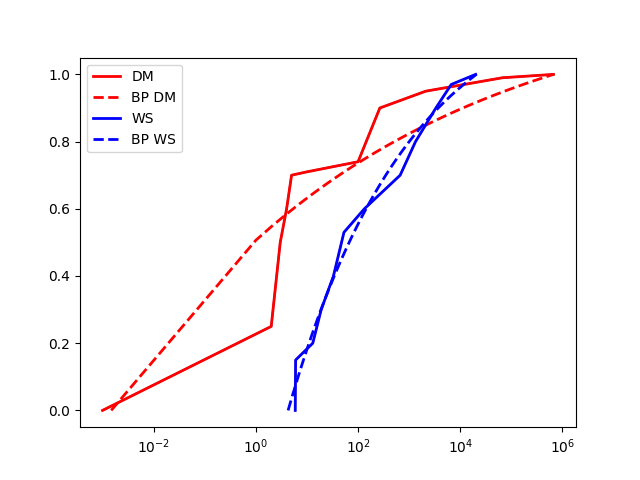
\includegraphics[width=\textwidth]{Chapter3/Figures/fits}
		\caption{CDF}
		\label{fig:cdfs}
	\end{subfigure}
   \hfill
   \begin{subfigure}[b]{0.49\textwidth}
   	\centering
   	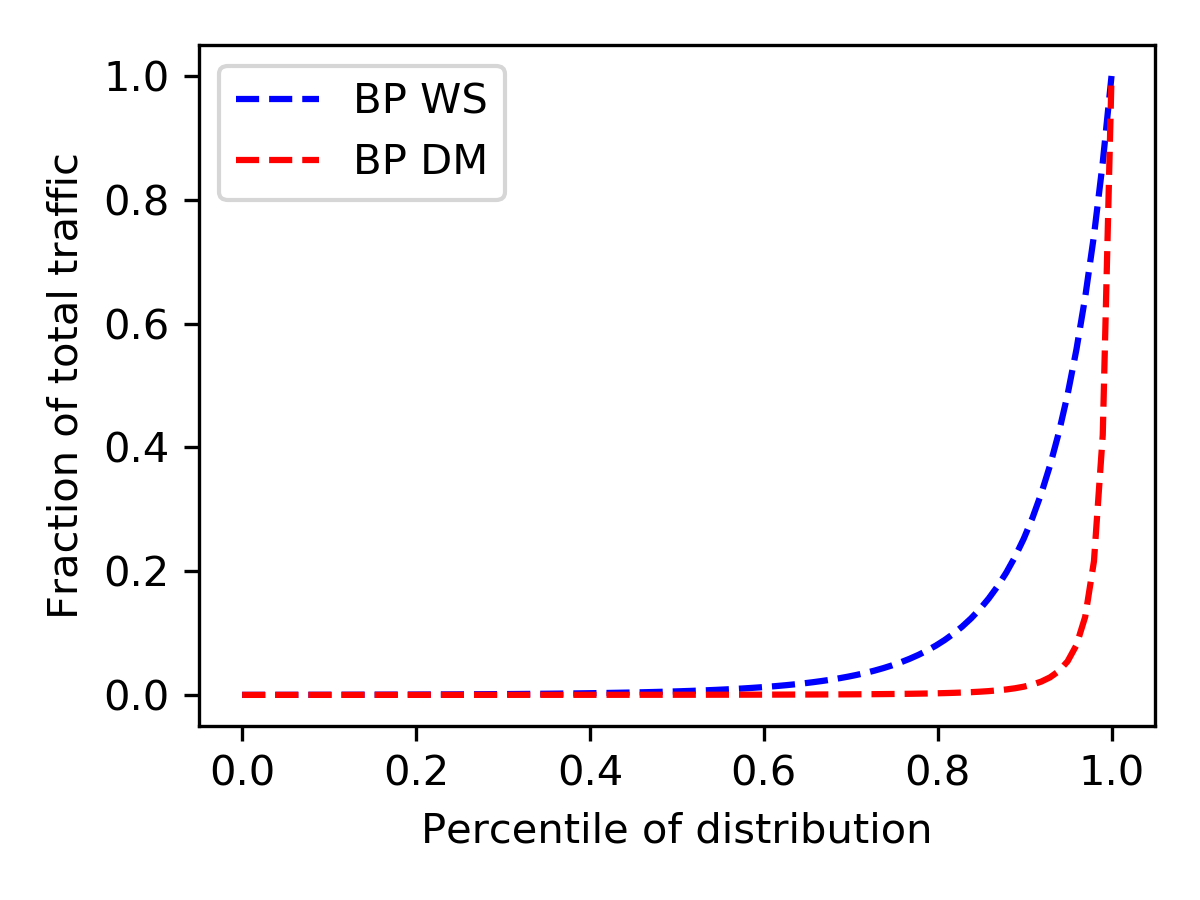
\includegraphics[width=\textwidth]{Chapter3/Figures/mwf}
   	\caption{MWF}
   	\label{fig:mwf}
   \end{subfigure}
	\caption{Workload properties}
	\label{fig:workloads}
\end{figure}
As expected, these distributions have a mix of short and long flows and both present the high-variability property typical of data center traffic (\S \ref{sec:traffic-properties}). Figure \ref{fig:cdfs} shows with solid lines the cumulative density function of the two empirical workloads, along with two analytical bounded Pareto distributions (dashed lines), whose parameters have been fitted to the corresponding empirical points. The bounded Pareto distribution is a truncated version of the Pareto distribution over the finite support $[u,t]$ and it is well-suited to model heavy-tail characteristics. It has three parameter: the lower extreme of its support $u$, the upper extreme $t$ and the shape parameter $\alpha$ that controls the weight of its tail. The analytical expression of its cdf $F(x)$ in the interval $[u,t]$ is:
\begin{equation}
	\label{eq:bpcdf}
	F(x) = \dfrac{1-\Big(\dfrac{u}{x}\Big)^{\alpha}}{1-\Big(\dfrac{u}{t}\Big)^{\alpha}}, \qquad 0 \le \alpha \le 2
\end{equation}
This distribution has been chosen to be used in the analysis due to some graceful properties. First of all, it is relatively easy to control its variability by a proper tuning of its parameter $\alpha$. Values of $\alpha$ close to 2 accentuate the heavy-tail property, while smaller values of $\alpha$ tend to regularize a bit its behavior. Second, being definite on a limited support it can be adapted to any minimum and maximum flow size in the datacenter. Third, the Pareto distribution is scale-invariant, meaning that normalized Pareto distributions remains Pareto. Nicely, this implies that the workloads observed by subsequent servers can be always modeled with the same probability distribution, only changing parameters. After all --- as seen in chapter \ref{ch:sdframework} --- these workloads  are conditional distribution obtained with simple normalizations. Last, its mean and its variance  --- which depend on $\alpha$ --- are finite, thus the problem of finding the shape parameter for any fixed first and second moment can be smoothly treated numerically. Specifically, for the bounded Pareto, the mean and the variance have the following expression:
\begin{align*}
\mathbb{E}[X] &= \dfrac{\alpha}{(1-\alpha)(t^{\alpha}-u^{\alpha})} (u^{\alpha}t - t^{\alpha}u) \\ \\
\sigma_X^2 &= \dfrac{\alpha}{(2-\alpha)(t^{\alpha}-u^{\alpha})} (u^{\alpha}t^2 - t^{\alpha}u^2)
\end{align*}
The best fit to the empirical distributions has been obtained with a simple Maximum Likelihood Estimator (MLE). The resulting parameters are reported for both the workloads. Let $X$ be the flow size random variable as usual, and write in short notation \textit{BP}($u,t,\alpha$) the bounded Pareto. 
\begin{align*}
	X_{WS} \sim& \text{\textit{BP}}(3, \, 29000, \, 0.125)\\
	X_{DM} \sim& \text{\textit{BP}}(0.1, \, 100000, \,0.26)
\end{align*}
The measurement unit for the extremes of the support in this case is kilobytes. The fitting error is higher for the data mining workload than for the web search. For low percentiles this is difficult to avoid because a very crude sampling is provided. In fact, on a total of 11 empirical points, 4 of them are for values above the 90th percentile. Instead, for high percentiles a better fitting likely could be obtained by weighting more the tail of the distribution. \\
The rightmost plot (Fig. \ref{fig:mwf}) completes the picture by showing the Mass-Weighted Function $M_w(x)$ \cite{mwf}. This can be seen as the probability that a byte picked at random belongs to a flow below a given percentile and it is used to characterize the variability of a distribution. Its name comes from its definition, where job sizes are weighted by their probability mass:
\[
M_w(x) = \dfrac{\int_{0}^{x} x f(x) dx}{\mathbb{E}[X]}
\]
It holds:
\[
\int\nolimits_{0}^{x} x f(x) dx \le \mathbb{E}[X]
\]
In other words, it is just the average normalized traffic injected by flows shorter than $x$. The figure has on the abscissa the percentile rather than the corresponding job size, to allow the comparison between workloads with different supports on the same axis. If $y$ is a given percentile, it is evaluated $M_w(F^{-1}(y))$. \\
In summary, both distributions exhibit high variability. In the web search case the largest 4\% of flows carry half of the total traffic, the data mining is even more skewed: 70\% of the flows are less than 8 packets only, but almost the entire load is sustained by a ridiculous percentage of flows of about 100MB of size. This suggests that the more challenging distribution to schedule is the web search, consequently it is the one that will deserve most of the attention. In fact, recall that an ideal flow-agnostic LAS scheduler guarantees lower and lower delays as the variability of the distribution increases, both on average and at high percentiles (\S \ref{sec:las}). The theory is confirmed pretty straightforwardly by the simulation results presented next. Moreover, the web search distribution is also a lot easier to simulate, since the very long tails of the data mining workload require protracted time-consuming simulations before being precisely reproduced. Long flows occur sporadically, however they give the main contribution to generate a desired load on the system. 

\subsection{Optimal traffic load balancing}
In previous discussions, it was already realized that the spatial diversity framework introduces strong implications on how the load is distributed on the switching fabric. We decided to solve an optimization problem with the goal of finding the optimal load balancing and then to treat sub-thresholds a posteriori (\S \ref{sec:decoupling}). Thus, we considered the abstraction of spatial diversity as a queuing system (\S \ref{sec:threesystemcomparison}) setting $N$=1 priority queue per server. With this setup all flow demotions correspond to shifting a flow from one server to the other. This way, the original problem of jointly optimizing inter and intra server demotion at once, has been simplified to finding the load balance that minimize the average flow completion time. \\
In this section we first start by analyze the simpler example of spatial diversity, where only two M/M/1 servers are deployed in parallel, each of them with only a single priority queue. In this case there is globally only one threshold, therefore it's possible to plot the shape of the cost function and to study its properties. It is worth remarking again that this threshold is a load balance threshold, therefore the following analysis will refer to the load balancing minimization problem, where there isn't any strict priority scheduler and all servers work in parallel with full capacity $\mu/K$. In other words, there is not any throttling that would assign only the residual capacity to the low priority server (already discussed in \S \ref{sec:decoupling}).  We start initially by solving the formulation for M/M/1 queues, then we will look for the solution of M/G/1 as well. For the sake of simplicity, we have implemented a total service rate $\mu = \mathbb{E}[X]$. In this way the average load fed in the system 
\[
\rho = \frac{\lambda}{\mu}\;\mathbb{E}[X]
\]
is given only by the flow arrival intensity $\lambda$.

\begin{figure}
	\centering
	\begin{subfigure}{.5\textwidth}
		\centering
		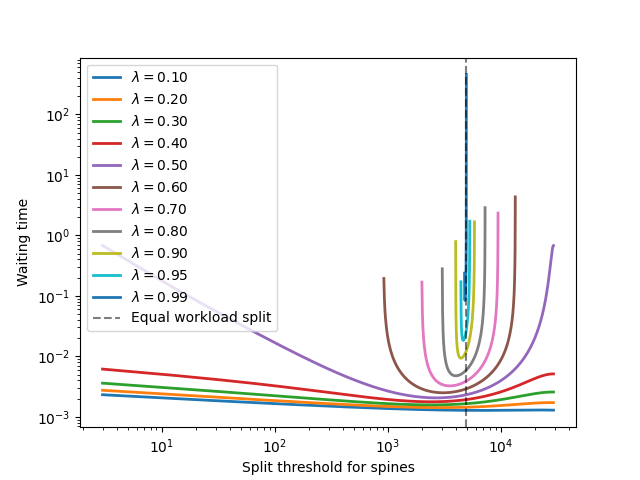
\includegraphics[width=.99\linewidth]{Chapter3/Figures/equal_workload_split_bpws}
		\caption{Optimal load balance threshold}
		\label{fig:cost-ws}
	\end{subfigure}%
	\begin{subfigure}{.5\textwidth}
		\centering
		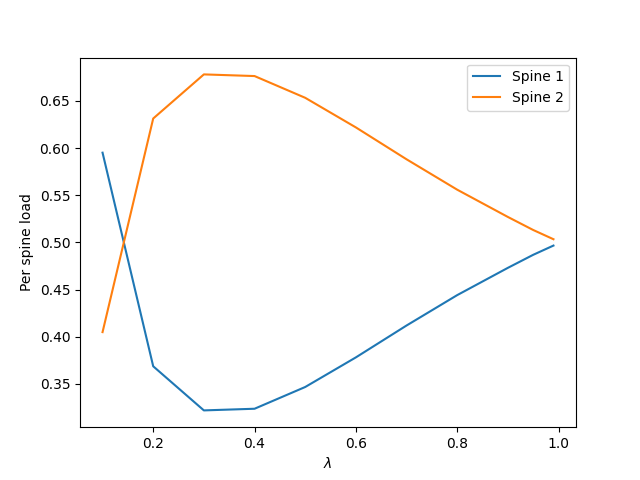
\includegraphics[width=.99\linewidth]{Chapter3/Figures/per_spine_load_bpws}
		\caption{Load distribution per-server }
		\label{fig:perspineload-ws}
	\end{subfigure}
	\caption{Web search workload. Simple case of $K$=2.}
	\label{fig:lbthreshold-ws}
\end{figure}

\begin{figure}
	\centering
	\begin{subfigure}{.5\textwidth}
		\centering
		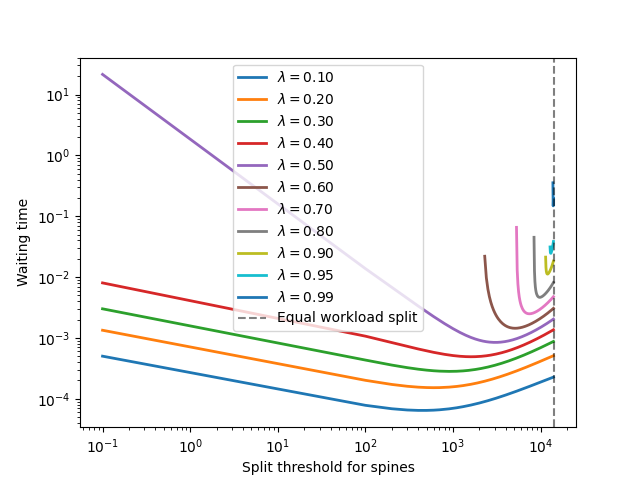
\includegraphics[width=.99\linewidth]{Chapter3/Figures/equal_workload_split_bpdm}
		\caption{Optimal load balance threshold}
		\label{fig:cost-dm}
	\end{subfigure}%
	\begin{subfigure}{.5\textwidth}
		\centering
		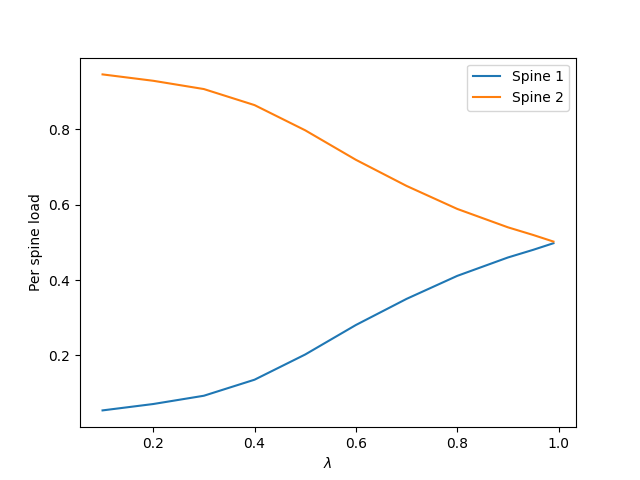
\includegraphics[width=.99\linewidth]{Chapter3/Figures/per_spine_load_bpdm}
		\caption{Load distribution per-server }
		\label{fig:perspineload-dm}
	\end{subfigure}
	\caption{Data mining workload. Simple case of $K$=2.}
	\label{fig:lbthreshold-dm}
\end{figure}%TODO per spine load measured or plugged threshold in equation? 
\subsubsection{Load balance on 2 parallel servers}
\label{sec:load-balance-2-servers}
In the basic case of $K$=2 parallel servers, it is possible to plot the average sojourn time when varying the load balance threshold. Figures \ref{fig:cost-ws} and \ref{fig:cost-dm} show how the cost functions look like, for the web search and the data mining workloads, respectively. All the axes are in log-scale and each curve represents a different normalized traffic $\lambda$. The vertical lines correspond to the split that gives perfect load balance, apportioning half of the traffic on the high priority server and half on the low priority one. This split may be interchangeably referred to as \emph{perfect split} or \emph{proportionate split} in the following. Figures \ref{fig:perspineload-ws}-\ref{fig:perspineload-dm} show in parallel the normalized traffic distribution on the two servers, corresponding to the optimal threshold. One phenomena is visible for both workloads, confirming previous intuitions. The optimal load balance threshold does not coincide, broadly speaking, with the proportionate split threshold. Depending on the traffic level at which the system is operated and the workload, the optimal threshold triggers an earlier or later demotion with respect to the perfect split case. Equivalently, the jobs are distributed unfairly between the two servers (Figures \ref{fig:perspineload-ws}-\ref{fig:perspineload-dm}). Imagine to connect the absolute minimums of the cost functions. For data mining, the imaginary line would be always in the leftmost side with respect to the proportionate split. That is, apart from loads close to saturation, the high priority server is kept as jobless as possible and the majority of work is sent to the low priority server. Remember that the problem formulation weighted the average sojourn times in the $i$-th priority queue with the percentage of flows with size between the thresholds $\alpha_{i}$ and $\alpha_{i+1}$. The objective was:
\[
\mathcal{T} = \sum_{i=1}^{N}\textcolor{red}{\theta_i} \sum_{j=i}^{N}T_j
\]
Since the data mining workload is highly dominated by short flows, they receive more importance and longer flows are moved soon to another path. Plenty of short flows carrying few bytes are kept on a separated link from medium sized flows and a couple of long flows. Thus, the result is not a surprise but it is coherent with the flow distribution. \\
Slightly different trend is observed for web search. Moving from low to high values of $\lambda$, the optimal threshold is initially greater than the perfect split axis, then switches to its left and finally the two coincide. This is clear from the load distribution on the two servers. In general, for web search the load remains more balanced between the two servers in respect to data mining. The more unbalanced split occurs at $\lambda$=0.3 where 70\% of the traffic is handled by the low priority server. Instead, data mining has much more extreme load subdivision, especially for $\lambda$=0.1. This is a consequence of the high variability of the workload: there is six order of magnitude difference between the shortest and the longest flow and there is a pronounced heavy-tail. Hence in order to have significant changes on the weights $\theta_i$ the threshold is moved significantly along the heavy-tail. In other words, the optimal threshold reroute few flows but lot of traffic on the low priority server. In fact, for $\lambda$=0.1 the absolute value of the optimal threshold is much smaller than the proportionate split threshold, however only a small fraction of flows fits into this gap. Also, for similar reasoning, the two workloads have different sensitivities to the load balance threshold optimization. In particular, the web search achieves appreciable FCT gains starting from medium loads only ($\lambda > 0.5$) with a factor 2 gain%\textcolor{red}{(TODO provide some numbers)}, 
whereas at low loads there is no practical difference with the proportionate split. On the contrary, the data mining distribution gives theoretically an order of magnitude %\textcolor{red}{(TODO provide some numbers)} 
lower waiting time even for $\lambda$=0.1. %This again reflects the extreme variability of the workload, that is comprised by a disproportionate number of short flows. %The perfect split would keep a lot of mice flows mixed with low priority flows of bigger size for protracted service time. Instead, 
Finally, for both cases the objective function becomes much more extremely curled and steep around the perfect split axis when the load approaches the saturation value 1.  As already remarked, this is inevitable in order to fully exploit all the available capacity offered by the two parallel servers. At so high load any other traffic split would overload one of the two links and strongly deteriorate the average completion time of the flows going through it. Consistently, the cost function grows very rapidly in the neighborhood of the perfect split threshold value. Indeed, the M/M/1 response time $T$ grows exponentially close to saturation. Its law (Figure \ref{fig:mm1-responsetime}) is:
\[
T \propto \dfrac{1}{1-\rho}
\]
\begin{figure}
	\centering
	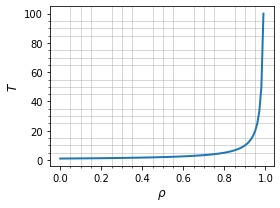
\includegraphics[width=0.4\textwidth]{ChapterSpatialDiversityFramework/Figures/mm1-response-time}
	\caption{M/M/1 response time}
	\label{fig:mm1-responsetime}
\end{figure}
\subsubsection{Validity of the model}
Summarizing, the above discussion confirms that the web search traffic is harder than the data mining to cope with. This is the reason why in the following some results are shown exclusively for this workload. 
Next, it is consolidated the validity of the stochastic optimization model with numerical flow level simulations, in particular it is shown the effective benefit of optimal load balancing. The underlying topology is again the simplest one, comprised of two parallel M/M/1 servers with no inner prioritization. The serving discipline is Processor Sharing (PS), implemented with a fluid model where parallel flows are served with equally subdivided bandwidth. 
The average normalized flow completion time (nFCT) has been considered as the primary evaluation metric.
\smallskip
\begin{tcolorbox}[title=Definition]
	\textbf{nFCT}: Given a fixed data center topology and pair of source-destination servers, \{$s$, $d$\}, define $FCT_{opt}(x)$ as the FCT achieved by a flow of length $x$ originated from $s$ and directed to $d$ in a completely empty DCN at load zero (excluding such a flow). Let $FCT(x)$ be the FCT of a flow of length $x$ in a DCN in the presence of other flows. Let $X$ be the set of all possible flow lengths. Define:
	\[
	nFCT = \sum_{x \in X} \small \frac{FCT(x)}{FCT_{opt}(x)} \normalsize.
	\]
\end{tcolorbox}
\smallskip
The normalized flow completion time is very similar in spirit to the average slowdown presented in Sec.\ref{sec:las}, but it is more handful as it is dimensionless. Its advantage is to put all flows on the same comparable scale, permitting a clean visual analysis of fairness with respect to flow size. By the way, this kind of evaluation is important to us, as spatial diversity mainly targets short and medium flows by augmenting the priority granularity. \\
Figures \ref{fig:optlb-ws}-\ref{fig:optlb-dm} report the nFCT gain obtained thanks to the sole load balance optimizer. 
\begin{figure}
	\centering
	\begin{subfigure}{.5\textwidth}
		\centering
		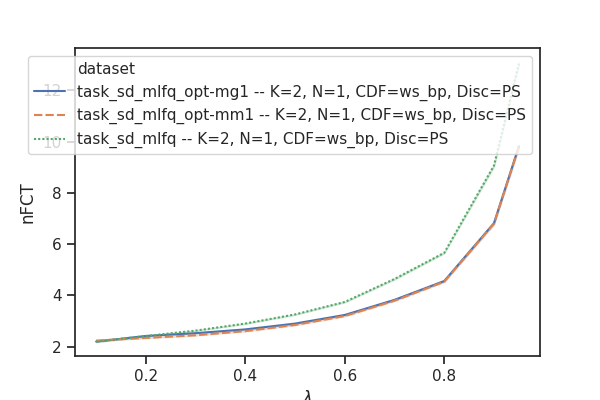
\includegraphics[width=1.05\textwidth]{Chapter3/Figures/ws_ps_comparison}
		\caption{nFCT comparison}
		\label{fig:optlbgain-ws}
	\end{subfigure}%
	\begin{subfigure}{.5\textwidth}
		\centering
		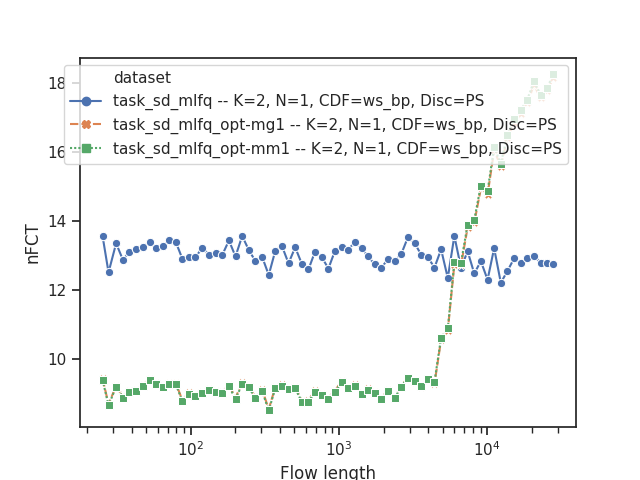
\includegraphics[width=\textwidth]{Chapter3/Figures/ws_ps_detailed.png}
		\caption{Per-flow length nFCT. $\lambda=$0.9}
		\label{fig:optlbgainvsflowsize-ws}
	\end{subfigure}%
	\caption{Web Search workload}
	\label{fig:optlb-ws}
\end{figure}%
\begin{figure}
	\centering
	\begin{subfigure}{.5\textwidth}
		\centering
		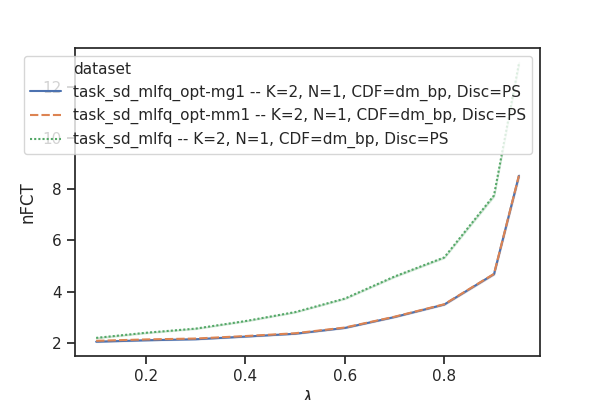
\includegraphics[width=1.05\textwidth]{Chapter3/Figures/dm_ps_comparison.png}
		\caption{nFCT comparison.}
		\label{fig:optlbgain-dm}
	\end{subfigure}%
	\begin{subfigure}{.5\textwidth}
		\centering
		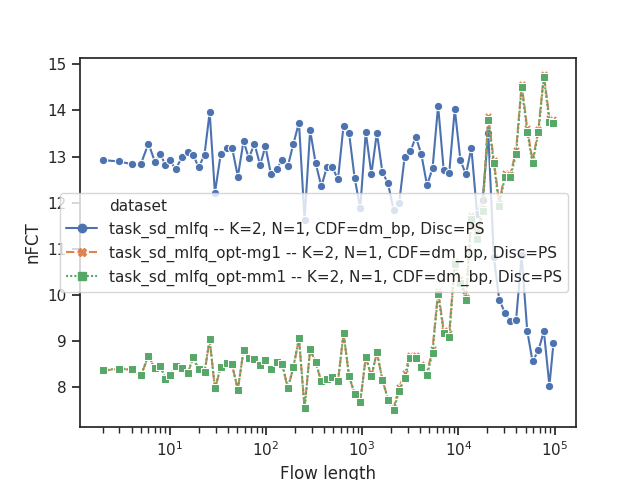
\includegraphics[width=\textwidth]{Chapter3/Figures/dm_ps_detailed.png}
		\caption{Per-flow length nFCT. $\lambda=$0.9}
		\label{fig:optlbgainvsflowsize-dm}
	\end{subfigure}%
	\caption{Data Mining workload}
	\label{fig:optlb-dm}
\end{figure}%
Two different scenarios are compared. Both adopt spatially-diverse MLFQ, but in one case the load balance threshold is optimized, in the other not. The former case is labeled as \texttt{SD-MLFQ-OPT}, whereas the latter as \texttt{SD-MLFQ}. Call $s_0$ and $s_1$ the two servers (i.e links/queues) and $\Omega$ the unique demotion threshold. Newly arrived flows always enter the system through $s_0$ as their attained service equals to 0, then they are rerouted to the link $s_1$ when server $s_0$ has transmitted $\Omega$ of their bytes. As expected, the benefits on the average completion times are more pronounced for the data mining distribution, at all loads (Figures \ref{fig:optlbgain-ws}-\ref{fig:optlbgain-dm}). Even so, appealing phenomena emerge when looking at the detailed breakdown of the response time versus flow size (Fig.\ref{fig:optlbgainvsflowsize-ws}-\ref{fig:optlbgainvsflowsize-dm}). First focus on the SD-MLFQ system without load balancing optimization and compare the blue curves. In web search, the normalized response time curve exhibits a constant plateau which testify a substantial invariance of the slowdown with respect to the flow length. Conversely, in data mining there is an abrupt transition to lower response times for flows longer than 20MB, which roughly corresponds to the demotion threshold adopted in this case. The difference is justified by the fact that the proportionate split threshold for data mining cuts the flow size CDF near the 99-th percentile, due to the oft-repeated heavy-tail characteristic of this workload. Therefore, only few long flows remain to share the processor of the low-priority server $s_1$.  Since the  nFCT captures the slowdown in respect to the ideal case where the flow is serviced alone, it is reduced when less flows contend the bandwidth. This is true as long as PS all servers use the PS discipline. \\
Next, let's concentrate on the spatial diversity with optimal load balancing (green curves), which is the real experiment needed in order to validate the model. The two workload perform similarly and have analogous trends. More importantly, the encouraging result is that short and medium flows indeed take advantage of spatial diversity, as they are sent through a less loaded path. For the data mining case, there is approximatively a 35\% gain for flows smaller than 6MB. The opposite happens to long jobs, which undergone the dual effect.
% TODO definition of main spatial diversity principles (bullet item list)
% TODO M/M/1 vs M/G/1 how implemented in practise? Assumed poisson arrivals but not true....what changed? How determined the variance of the job for subsequent servers? 
\subsubsection{Finding optimal load balance with Basin-hopping}
So far the only scenario that has been investigated is the simple case of two parallel servers without sub-thresholds. This was useful to get confident with the relationships between load balance and the spatial diversity demotion mechanism. However, in the more general setting there might be much more parallel servers and at least two priority levels per server. The total number of thresholds was reduced by decoupling the load distribution by the server-local prioritization. Thus, the total complexity only depends on the number of servers $K$. Unfortunately, it is still typically high. 
%\textcolor{red}{TODO basin hoppin brief description (GERMAN) + parameter setting of the solver (GERMAN) + solution time plot descrioption (ALE)}
Basin-hopping is a meta-heuristic which provides means of solving non-convex optimization problems.
It operates on an iterative basis by selecting random starting point in possible solution state-space and performing local minimization. 
Subsequently the process is repeated by "hopping" to a different point and re-performing minimum search.
We consider BFGS as a local minimization algorithm, we set a step size equals to 100 for random perturbation as it was empirically found to be a good trade-off between convergence speed and accuracy.
We then perform 300 iterations for each point in \textbf{figura con i load} on a Intel i7-7700k with 16GB of RAM.
% dire python scipy solver
% TODO citare basin hoppin e pso heuristics (some parameters used, bla bla)
% TODO why complexity is higher at load 0.6 ???
\section{Dimensioning spatial diversity}
In the previous section it was laid down the basic framework of spatial diversity. It was remarked the fact that adopting spatial diversity translates into a priority-driven load balancing. At the same time were collected encouraging results about the effectiveness of the optimal load balancing. It was discussed the impact of two workloads commonly used as a benchmark in literature. Then, it was solved the optimal load balancing problem for up to $K$=9 parallel servers ans shown that for large topologies we may incur in overwhelming complexity. In all the simple experiments carried out, the servers were always configured with Processor Sharing service discipline and without priority queues.

This section aims to provide answers to principally two things. The first one is the behavior of the priority-driven load balancing when increasing the number of server $K$ up to 9 parallel servers. Thus, we try to evaluate the effects of the load balance thresholds alone with bigger topologies, initially disregarding sub-thresholds again. Second, it is treated the integration of the priority-driven load balancing with the legacy MLFQ system. In practice, it is considered the general case where each server has many PQs on its interfaces used in strict priority. As it will be explained shortly, it turns out that for both attempts, the performances of the system are highly correlated with the adopted servicing policy. The two considered cases are the FIFO (FCFS) servers and the usual PS servers. 

\subsection{Effects of SD-rank and PQ granularity}
\label{sec:dimensioning-spatial}
First it is addressed the first question: what are the effects of augmenting the spatial diversity \emph{rank}? 
\begin{tcolorbox}[title=Terminology]
	\textbf{SD-rank}: Given a data center topology with $S$ spines --- or the equivalent system of parallel M/M/1 servers where is applied priority-driven load balancing, that is each server handle a group of priority and a flow is routed depending on its assigned priority. Let's define the spatial-diversity rank (SD-rank) as the number $K$ of servers which handle different priorities. 
\end{tcolorbox}
The spatial diversity ranks tells how many M/M/1 servers (or group of servers) are considered to be used to implement spatial diversity. For example, suppose there are 4 parallel servers available $s_0$, $s_1$, $s_2$, $s_3$. Consider these two possibilities. 
\begin{enumerate}
	\item \textbf{Rank 2}. The four servers are grouped in two pairs, say $(s_0, s_1), (s_2,s_3)$. Spatial diversity demotion is applied at pair level. This means there is only one load balance threshold $\Omega$. When the longest flow enters the system, it is sent at random either on $s_0$ or $s_1$. As soon as the flow has received service $\Omega$ it is demoted, again randomly, either on $s_3$ or $s_4$. In other words, this can be seen as a system of only two parallel servers with twice the capacity each, where only one rerouting happens to the longest flow. 
	\item \textbf{Rank 4 \textit{(full-rank)}}. The servers are not grouped in any way. All servers participate to the priority-driven load balance. Therefore, there are 3 thresholds and the longest flow it is rerouted three times.
\end{enumerate}
In the next experiments (Fig.\ref{fig:lb-var-K-fifo}) is evaluated the full-rank spatial diversity system for three topologies, corresponding to $K=3$, $K=5$, $K=9$ and for two serving policies: PS and FIFO. The number of priority queues $N$ is still one per server. Remember that the numerical simulator is a job level simulator, thus flows are not fragmented in packets anyhow. This means that the FIFO policy is absolutely non-preemptive for jobs in the same priority queue. The service of a flow cannot be interrupted and flows arriving in the meanwhile are queued back in a first-in first-out order. Instead, the PS discipline subdivides the available capacity among all flows present in the system with a fluid approximation. Thus, a fresh flow share immediately the service rate granted to its priority queue with other flows in the same queue. 
\begin{figure}
	\centering
	\begin{subfigure}{.5\textwidth}
		\centering
		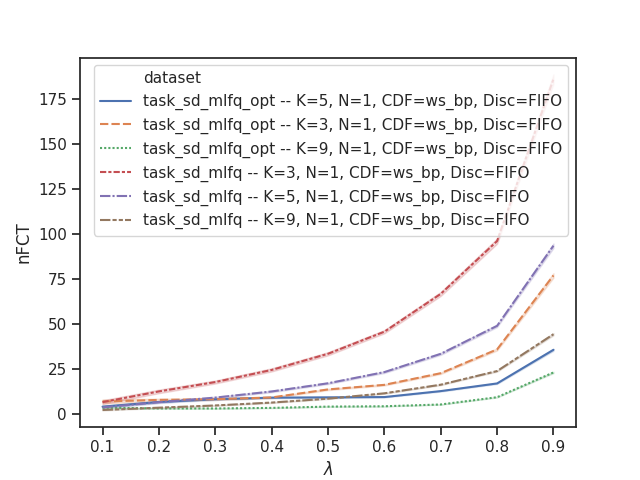
\includegraphics[width=0.99\textwidth]{Chapter3/Figures/lb_opt_vs_nopt_comparison}
		\caption{nFCT comparison}
	\end{subfigure}%
	\hfill
	\begin{subfigure}{.5\textwidth}
		\centering
		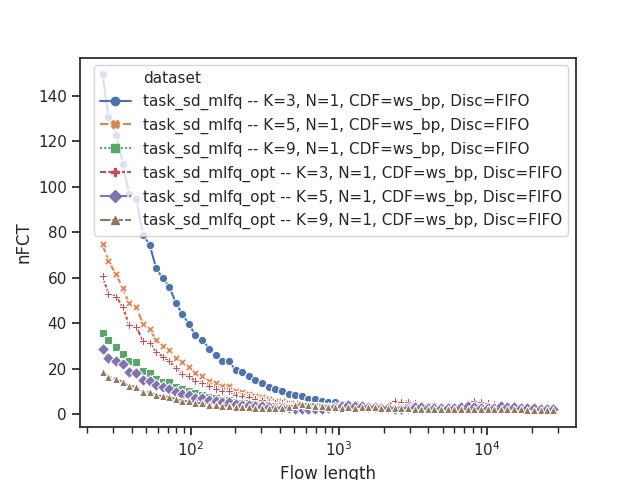
\includegraphics[width=0.99\textwidth]{Chapter3/Figures/lb_opt_vs_nopt_detailed}
		\caption{Per-flow length nFCT ($\lambda$=0.9)}
		\label{fig:lb-var-K-fifo-detailed}
	\end{subfigure}
	\caption{Web Search workload and FIFO discipline at 99\% confidence interval.}
	\label{fig:lb-var-K-fifo}
\end{figure}
\begin{figure}
	\centering
	\begin{subfigure}{.5\textwidth}
		\centering
		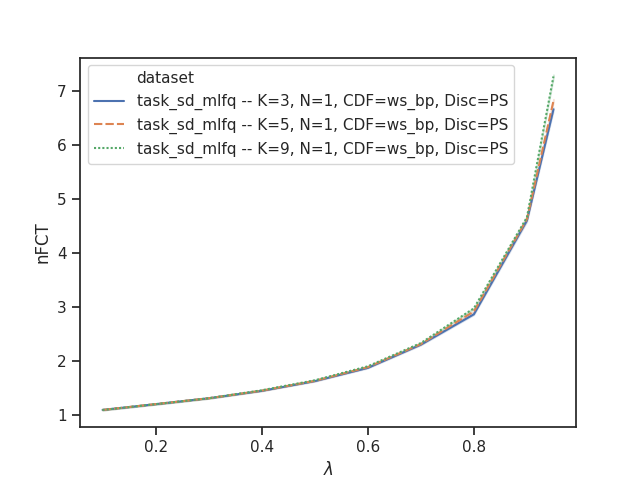
\includegraphics[width=0.99\textwidth]{Chapter3/Figures/lb_opt_vs_nopt_comparison_fifo}
		\caption{nFCT comparison}
	\end{subfigure}%
	\hfill
	\begin{subfigure}{.5\textwidth}
		\centering
		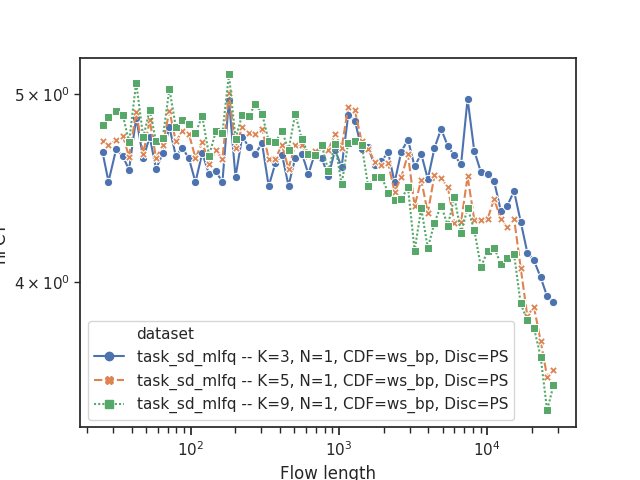
\includegraphics[width=0.99\textwidth]{Chapter3/Figures/lb_opt_vs_nopt_detailed_ps}
		\caption{Per-flow length nFCT ($\lambda$=0.9)}
		\label{fig:lb-var-K-ps-detailed}
	\end{subfigure}
	\caption{Web Search workload and PS discipline at 99\% confidence interval.}
	\label{fig:lb-var-K-ps}
\end{figure}
%TODO when N=2 and FIFO what's the policy?
These experiments were carried out both with and without the optimized load balance thresholds. Whenever load balance thresholds are not optimized, it is used the proportionate split criterion. Experiment are shown for the web search workload only, which is the more challenging to handle. The first very positive observation is that, whatever the number of servers, the optimal load balance wins over the proportionate split. This again confirms the validity of the queuing model formulation for load balancing. 
The FIFO policy is clearly unfair with respect to short flows (Fig.\ref{fig:lb-var-K-fifo-detailed}). This is because without preemption a single elephant flow could starve a myriad of short flows. This does not happen with PS, because short flows always share the processor with other longer flows. Indeed, in absolute terms the PS discipline overcome of two order of magnitude FIFO, remarking the fact that under the assumption of high variability of the distribution, it is better to adopt a PS policy. The unfairness of FIFO is mitigated when increasing the spatial diversity rank, as long flows are demoted earlier and leave quickly high priority servers. Notably, for a fixed $K$, having $N$=1 priority queue is the worst case from the point of view of mice flow starvation. With $N$>1 PQs, the service received by a flow on each server would be broken in multiple phases, each on a different priority queue. Since the PQs are scheduled in Strict Priority order and newly arrived flows enter in high priority, a short flow behind longer ones would have to wait only until the demotion at lower priority of the flows ahead. Somehow the demotion preempts the long flows, and weaken the impact of having a FIFO policy on the PQs themselves. \\
Not surprisingly, when increasing the rank there is not a significant change in the average flow completion time with PS. In the web search distribution a relevant role is played by medium flows. Thus, increasing the number of inter-server demotions without any intra-server demotion hasn't any effect on FCT minimization. Medium flows stay anyway with elephant flows, only across more parallel servers. This clearly indicates that the priority dependent load balance alone is not enough with PS. On the other hand, for higher rank we start observing on elephant flows the same trend that was observed in Fig.\ref{fig:optlbgainvsflowsize-dm} for the data mining workload but not for the web search. In that section, (\S \ref{sec:load-balance-2-servers}) we had only 2 parallel servers and we argued that this gain for the elephant flows happened because only few simultaneous flows shared the processor of the lower priority server. Here the same happens also for the web search distribution, since there are enough demotions to truncate the distribution at high percentiles and leave few flows for low priority servers.
%Finally, it is possible to As a trivial example, suppose to schedule two flows $f_1, f_2$ of size 10 bits/bytes/packets,... Denote as $T(f_i)$ the average flow completion time of flow $i$, expressed in transmission slots. FIFO scheduling would give:
%\[
%	T_{FIFO}(f_1) = T_{FIFO}(f_2) = \dfrac{10+20}{2} = 15
%\]
%Instead, PS scheduling would be worse:
%\[
%T_{PS}(f_1) = T_{PS}(f_2) = \dfrac{19+20}{2} = 19.5
%\]
%Remember that subsequent servers observe cut workloads, whose heavy-tailed property is gradually destroyed. In other words, the flow size distributions fed in low priority servers have reduced variability (Fig. \ref{fig:cdfs}). This is a clear downside for PS policy.

The study of the system with increased number of priority queues led to even more surprising results. This step really integrates the spatial diversity in the legacy MLFQ system with many priority levels. Here it is reported only the Processor Sharing discipline for the reasons explained few lines above: it is clear that for FIFO increasing $N$ would further reduce the average flow completion time. A numerical proof confirming this fact will be shown in the last section \S \ref{sec:final-comparison} of the chapter during the final comparisons of SD-MLFQ with ES-N. \\
Figure \ref{fig:sdmlfq-variable-N} is a key result that will uncover potential bottlenecks of SD-MLFQ. In this experiments are compared the average flow completion times of the system with fixed $K$=4 and variable $N$. Load balance thresholds are not optimized in this case, but are set to grant the proportionate split of the traffic on the four parallel servers. The sub-thresholds have been assigned with the simple ES-N variation for spatial diversity (\S \ref{sec:subthresh-with-sd}). Very interestingly, this numerical results provide a different perspective on the best granularity of priority queues per server when introducing spatial diversity. While on the systems that approximate LAS or SRPT schedulers \cite{pias, pFabric}, increasing the number of priority queues is always beneficial, it is not so when spatial diversity is adopted. At low load there is not a visible difference among the simulated scenarios. However, at high load the best average nFCT is attained with $N$=2 priorities per server (dashed orange curve). The peculiar phenomenon is the behavior of the case $N$=8 (red curve), whose corresponding nFCT starts to increase consistently above $\lambda=0.8$. 
\begin{figure}
	\centering
	\begin{subfigure}{.5\textwidth}
		\centering
		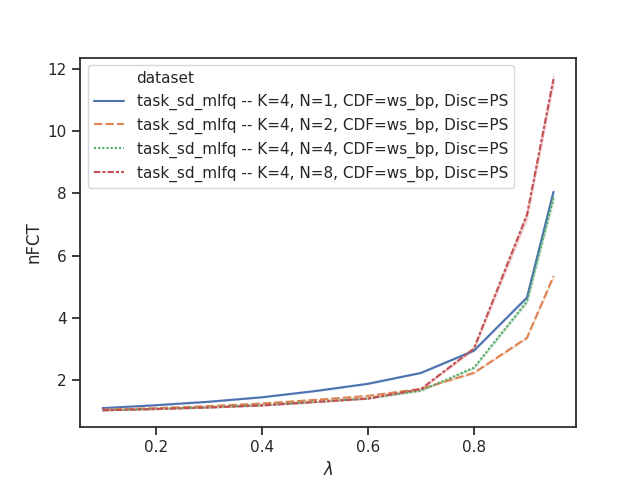
\includegraphics[width=0.99\textwidth]{Chapter3/Figures/sd_mlfq_k4_comparison.png}
		\caption{nFCT comparison}
		\label{fig:sdmlfq-variable-N-fct}
	\end{subfigure}%
	\hfill
	\begin{subfigure}{.5\textwidth}
		\centering
		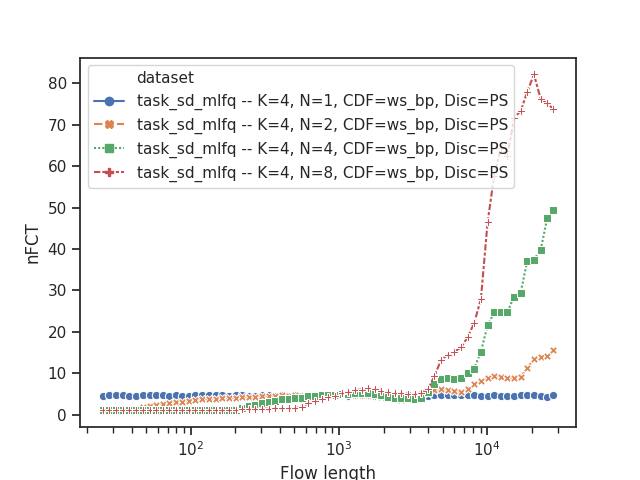
\includegraphics[width=0.99\textwidth]{Chapter3/Figures/sd_mlfq_k4_detailed.png}
		\caption{Per-flow length nFCT ($\lambda$=0.9)}
		\label{fig:sdmlfq-variable-N-fct-detailed}
	\end{subfigure}
	\caption{Effects of intra-server demotion with spatial diversity. Results shown for web search workload, PS and fixed $K=4$. Results plotted with 99\% confidence interval.}
	\label{fig:sdmlfq-variable-N}
\end{figure}
From the detailed breakdown of Fig.\ref{fig:sdmlfq-variable-N-fct-detailed}, it is evinced that the most severe degradation happens to long flows. As a general trend, an higher number of priorities per server is reflected in a more pronounced raise of the job response time of long flows. At the same time, coherently with the scheduling theory of LAS (\S \ref{sec:las}) and the results of PIAS, flows between 100KB and 1MB (medium size flows) are improved. However, long flows suffer an unacceptable penalty, which globally makes also the average worse.  \\
We repeated the same experiment with the smallest possible rank that guarantees the applicability of spatial diversity, that is $K$=2. The results are shown in Fig. \ref{fig:sdmlfq-variable-N-K2}. 
\begin{figure}
	\centering
	\begin{subfigure}{.5\textwidth}
		\centering
		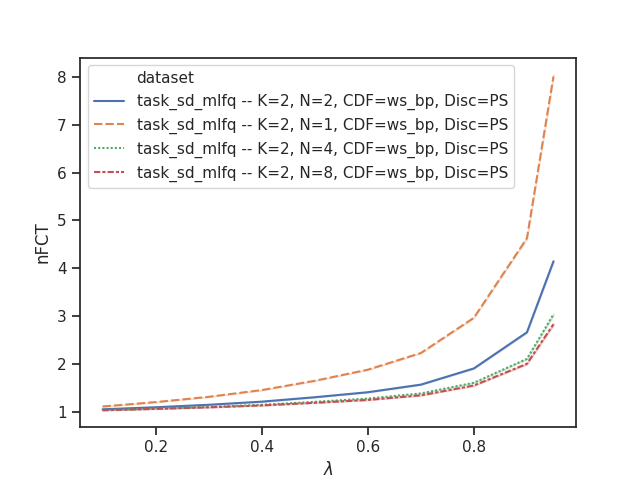
\includegraphics[width=0.99\textwidth]{Chapter3/Figures/sd_mlfq_k2_comparison.png}
		\caption{nFCT comparison}
		\label{fig:sdmlfq-variable-N-fct-K2}
	\end{subfigure}%
	\hfill
	\begin{subfigure}{.5\textwidth}
		\centering
		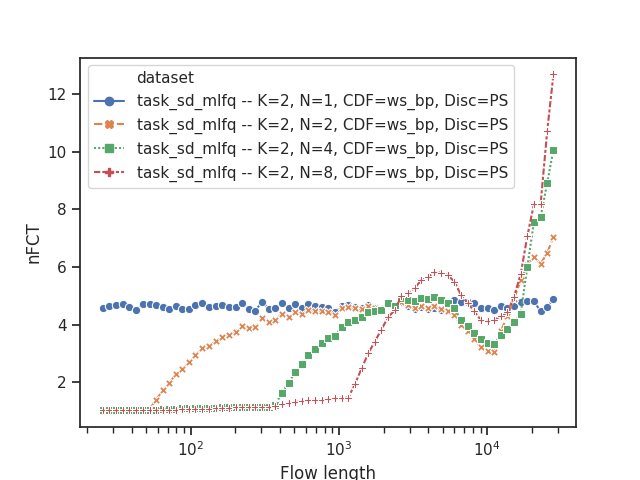
\includegraphics[width=0.99\textwidth]{Chapter3/Figures/sd_mlfq_k2_detailed.png}
		\caption{Per-flow length nFCT ($\lambda$=0.9)}
		\label{fig:sdmlfq-variable-N-fct-detailed-K2}
	\end{subfigure}%
	\caption{Effects of intra-server demotion with spatial diversity. Results shown for web search workload, PS and fixed $K=2$. Results plotted with 99\% confidence interval.}
	\label{fig:sdmlfq-variable-N-K2}
\end{figure}%
Intriguingly, the problem on longer flows starts to reveal, but with less intensity. This suggests some correlation between the spatial diversity rank and the critical behavior of long flows, especially when there are 8 priority queues per server.  Short and medium flows experience exactly the same trend as in the case $K$=4, but in this case it is visually more clear (Fig.\ref{fig:sdmlfq-variable-N-fct-detailed-K2}) because it is not squeezed by the scale of y-axis. 
\subsection{Impairments of spatial-diversity}
Summarizing, the previous experiments leave the following remarks as concerns the Processor Sharing (PS) discipline:
\begin{itemize}
	\item \textbf{Remark 1. \textit{Impact of PQ granularity}.} Whatever the spatial diversity rank (number of parallel servers across the which is applied spatial diversity), there is a nFCT penalty for long flows in using more than $N$=2 priority queues per server.
	\item \textbf{Remark 2. \textit{Impact of SD-rank}.} When $N>1$, that is when intra-server demotion is applied, increasing the spatial diversity rank rapidly exacerbates the nFCT impairments on long flows. The performance drop may become unacceptable and dominate the behavior of the average FCT curve.
\end{itemize}
Such an extreme behavior on long flows was worth of extra-attention. In particular, it brings up two important questions: why does it happen? Is the best choice to continue demotion also in low priority servers?
We concern why spatial diversity exacerbates the unfairness of the scheduler with respect to longer flows. The fact that long flows are penalized is not new. Both LAS, the theoretical scheduling policy, and MLFQ, its approximation with priority queues, suffered the problem of long flows starvation. Nonetheless, the spatial diversity presents a peculiar impairment that worsen the performances if the size of the topology --- precisely the SD-rank --- grows. We identified two causes of the problem: demotion in low priority servers and flow synchronization. Unfortunately, both of them are either originated or amplified by the spatial diversity. 
\subsubsection{Demotion in low priority servers}
We ask whether it is meaningful to exploit all available priority queues in low priority servers for flow demotion, or not. We addressed this problem by looking at the simple scenario of $K=N=2$ with the web search workload. This setting allows to have a single load balance threshold and a single sub-threshold in each server $s_1,s_2$. Then, we tried to optimize the sub-threshold on the low priority server, for any possible load balance threshold. This step was easily treatable numerically with a brute-force minimization, as there is only one sub-threshold.
\begin{figure}
	\centering
	\begin{subfigure}{.5\textwidth}
		\centering
		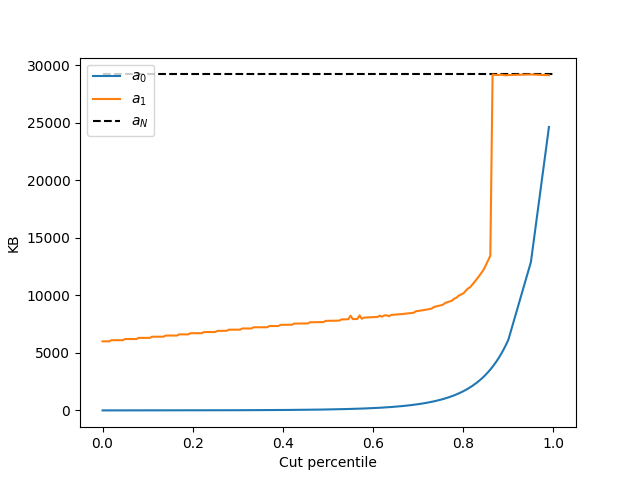
\includegraphics[width=0.99\textwidth]{Chapter3/Figures/cut_demotion}
		\caption{Optimal sub threshold for $s_2$ ($\lambda=0.99$)}
		\label{fig:opt-subth-lowpserver}
	\end{subfigure}%
	\hfill
	\begin{subfigure}{.5\textwidth}
		\centering
		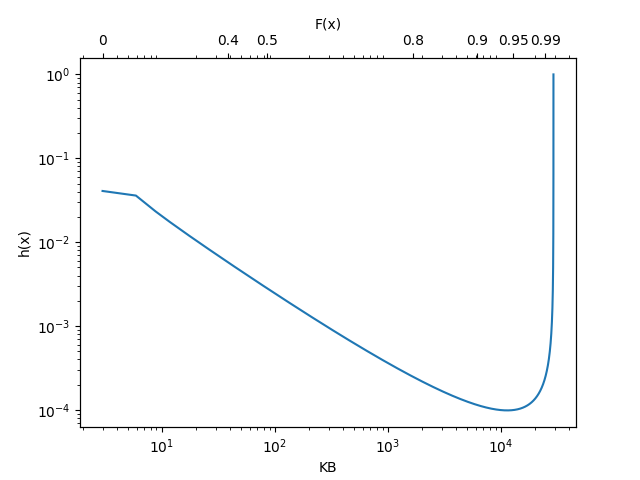
\includegraphics[width=0.99\textwidth]{Chapter3/Figures/hazard_pareto}
		\caption{Hazard function.}
		\label{fig:hazard}
	\end{subfigure}%
	\caption{WS workload}
\end{figure}%
Figure \ref{fig:opt-subth-lowpserver} shows the results. On the abscissa there are the cut percentile at which the load balance threshold truncate the job size distribution. The lower bound (blue curve) is the load balance threshold value, varying in order to cut the workload cdf at a given percentile.  The upper bound (black dashed line) is the length of the longest job in the workload. Finally, it is shown the optimal sub-threshold of the low priority server $s_2$ (orange line), computed for each imposed cut. The notable result is that starting from nearly the 90-th percentile, it is not convenient to use PQs on the low priority server for demotion. Indeed, the optimal sub-threshold saturates to the extreme of the support. This is coherent with the increasing hazard function at high percentiles. Indeed, it was discussed (\S \ref{sec:las}) that LAS scheduling is convenient when the hazard rate $h(x)$ is a decreasing function.\\
This experiment also explained why the performances are so bad when the dimensions of the system increase. The heavy-tail of the DC-wide workload is progressively reduced as considering lower and lower priority servers. Under this condition, it is not recommended to schedule with LAS discipline, thus many intra-server demotion are a downside. Intuitively, since lower priority servers receive only jobs corresponding to high percentiles, on these servers long flows cause protracted starvation of longer elephant flows. 
\subsubsection{Flow synchronization}
The second issue we have identified is flow synchronization. Consider the topology with $K$=5 and $N$=2. We plot the CDF of the flow inter-arrival time, that is the distribution of the time elapsed between two consecutive job arrivals. 
\begin{figure}
	\centering
	\captionsetup{width=.75\linewidth}
	\begin{subfigure}{.5\textwidth}
		\centering
		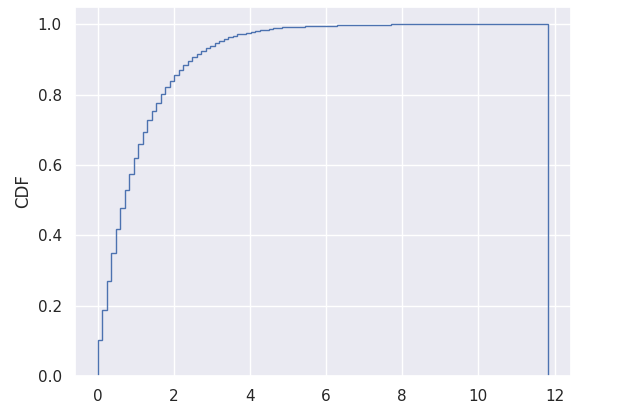
\includegraphics[width=0.99\textwidth]{Chapter3/Figures/inter_arrival0_PS}
		\caption{CDF at $s_1$}
		\label{fig:iatimes-ps-s1}
	\end{subfigure}%
	\hfill
	\begin{subfigure}{.5\textwidth}
		\centering
		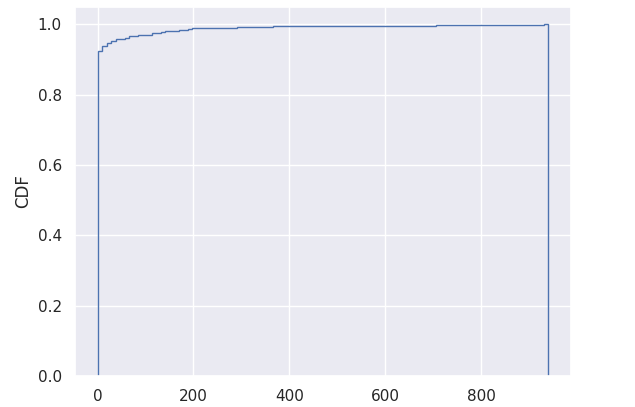
\includegraphics[width=0.99\textwidth]{Chapter3/Figures/inter_arrival4_PS}
		\caption{CDF at $s_5$}
		\label{fig:iatimes-ps-s5}
	\end{subfigure}%
	\caption{Flow synchronization with PS discipline. Flow inter-arrival distributions at highest and lowest priority servers.}
	\label{fig:iatimes-ps}
\end{figure}%
As usual the notation $s_i$ indicates the servers, from higher to lower priority. By looking at the distribution on the lowest priority server $s_5$, there is an anomalous spike at 0ms inter-arrival, that spans the y-axis up to the 90-th percentile (Fig.\ref{fig:iatimes-ps-s5}). This is strange because all flows enter the system from $s_1$, hence we expected a flatter cumulative function, at least at the beginning. Instead, its shape discloses bursts of flow arrivals, with many of them arriving synchronized at the same time instants. \\
We explain this synchronization as a joint result of processor sharing, strict priority and flow demotion. Consider a generic set of flows $\mathcal{F}$, whose sizes are such that the all flows end their service in $s_5$. Denote with $Q_i^j$ the $i$-th priority queue of the $j$-th server, with the usual order and notation followed in the theoretical model of spatial diversity (\S \ref{sec:complete-model}). Flow $\tilde{f}$ enters the system through $s_1$ and starts its service. Denote with $\mathcal{F}^\prime$  all flows $f \in \mathcal{F} \setminus \{\tilde{f}\}$ entered the system before $\tilde{f}$. Instead, use $\mathcal{F}^{\dprime}$ for all flows $f \in \mathcal{F} \setminus \{\tilde{f}\}$ arriving after $\tilde{f}$ but still while $\tilde{f}$ is served by the first server. Flows in $\mathcal{F}^{\dprime}$ either share the processor with $\tilde{f}$ in the high priority queue $Q_1^1$ or are served with higher priority of $\tilde{f}$ because this is already in the lowest priority queue $Q_2^1$.  In both cases, $\tilde{f}$ is the first to be shifted to the lowest PQ and at this point happens the synchronization. As a matter of fact $\tilde{f}$ doesn't leave the lowest PQ until all flows $f \in \mathcal{F}^{\dprime}$ do. First it waits them in $Q_2^1$ because of strict priority scheduling among PQs, then it shares the processor with them. When finally $\tilde{f}$ is rerouted to the subsequent server $s_2$, those flows in $\mathcal{F}^\prime$ that are yet served in $s_2$, again synchronize themselves with --- at least --- $\tilde{f}$.  In other words, the combination of spatial diversity, processor sharing and strict priority create on-off bottlenecks that lead to synchronization. This explanation is validated by the fact that in case of FIFO we do not observe any of this effect. Figure \ref{fig:iatimes-fifo} reports the inter-arrivals at the lowest priority servers $s_5$; for $s_1$ it is appropriately identical to the one obtained with PS.
\begin{figure}
	\centering
	\begin{subfigure}{.45\textwidth}
		\centering
			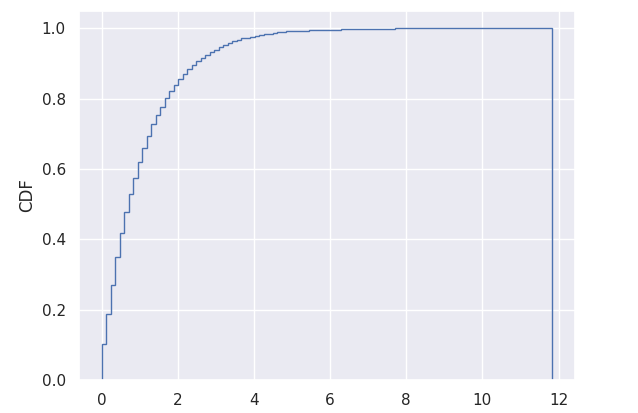
\includegraphics[width=0.99\textwidth]{Chapter3/Figures/inter_arrival0_FIFO}
		\caption{CDF at $s_1$}
		\label{fig:iatimes-fifo-s1}
	\end{subfigure}%
	\hfill
	\begin{subfigure}{.45\textwidth}
		\centering
		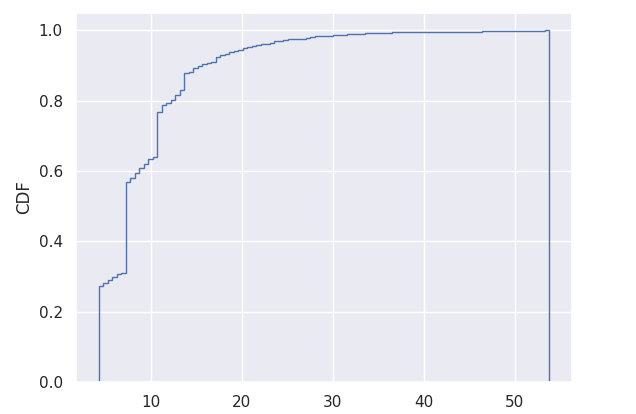
\includegraphics[width=0.99\textwidth]{Chapter3/Figures/inter_arrival4_FIFO}
		\caption{CDF at $s_5$}
		\label{fig:iatimes-fifo-s5}
	\end{subfigure}%
	\caption{FIFO does not suffer flow sync. CDF of inter-arrivals shown only for $s_5$}
	\label{fig:iatimes-fifo}
\end{figure}%

We think that this flow synchronization arises also in the system without spatial diversity and it is something not highlighted by authors of PIAS. Instead of showing at server level, we think that bursts arrivals could occur at priority queue level, especially when $N$ is large. However, since lower priority queues are served in strict priority only when high PQs are empty, we guess that these bursts are also less penalizing. \textcolor{red}{QUAL'ERA IL COMMENTO DI ANDREA ? CHE IN UNA RETE A PACCHETTO PROBABILMENTE NON SI VEDE COSI TANTO?? PERCHE' ? PERCHE' IL FLUSSO NON CE L'HAI TUTTO SUBITO MA LE TCP SOURCES TE LO MANDANO SEGMENTATO?}
\subsection{Final comparison}
%\textcolor{red}{Final comparison with ES-N (no spatial). Show plots and resume table}.

\chapter{Evaluation in simulated Data Center Network}\label{ch4}
The last chapter of this work is the evaluation of our proposal in a packet network. We configured a DCN network in a simulated environment, where now the protocol stack is fully implemented. We worked with the open-source discrete event simulator OMNeT++ \cite{omnetpp} and the INET library \cite{inet}, which provides readily deployable components for the TCP/IP stack, link layer and physical layer protocol implementations, as well as models for QoS provisioning. In order to test spatial diversity we extended and customized some of the library components. The most relevant among of these modifications will be reported in this chapter to allow easy reproducibility. Indeed, we dedicate the first section (\S \ref{sec:opp-setup}) to an in-depth description of the simulation methodology and the configuration of the network components and their interactions. Then, we will analyze the results and draw the final conclusions. 
\section{Simulator setup}
\label{sec:opp-setup}
OMNeT++ is a discrete-event simulator, based on message passing. Essentially, the events are represented by messages which are stored in a priority queue. The user can schedule events by creating a message with associated a timestamp, which indicates the moment in time when events need to be simulated and corresponds to the message priority in the queue.  The events are sorted in ascending order of timestamps.  Obviously, there isn't correspondence with the real time, instead all timestamps refer to a simulated time. Therefore, all events are executed at CPU speed and the virtual simulation time is set artificially to the timestamp of the last event popped from the queue. \\ OMNeT++ separates the definition of the model components from their actual implementation. It provides a descriptive language to define which components to include in the simulation model and possibly to define interconnection among them. The interconnections allow different modules to communicate with message passing. Separately, the user can implement the actual behavior of such components. For each of them it is possible to customize the routines to handle events, schedule new events and pass messages to other modules.

We worked in Ubuntu 16.04 environment, using OMNeT++ v.5.2.1 and INET v3.6.4. 
The goal of this section is to explain the setup we used on our simulator and provide implementation details, eventually useful for hands-on experiments with this system. 
\subsection{Traffic generation}
We consider a standard leaf and spine Ethernet-based topology, with only two layers. All hosts in the topology are directly connected through a single 1Gbps links to ToR switches, that comprises the first layer. Then, all ToRs are connected to all spines (second layer), forming a bi-partite graph structure. Also these links are configured at 1Gbps speed. We do not apply any over-subscription, therefore the aggregate bandwidth of all access links equals the bisection bandwidth. The topology and the nomenclature is shown in Fig. \ref{label}.
\begin{figure}
	\centering
	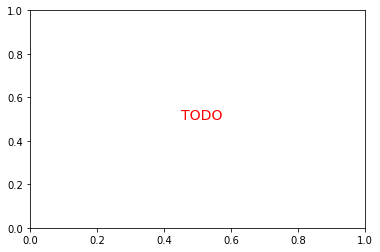
\includegraphics[width=0.5\textwidth]{Chapter3/Figures/todored}
	\caption{Data center topology used in simulations}
\end{figure}%
\\The first point is to generate a given amount of traffic. We want the hosts to fed the DCN with a given offered load $\rho$ defined as the average traffic offered to the switching fabric normalized to the bisection bandwidth. All hosts in the network have a single traffic source application and a single traffic sink application. Flows arrive at traffic sources according to a Poisson process with intensity $\lambda$ and are sent to a traffic sink belonging to another server chosen uniformly at random. Every new flow size is drawn from a given distribution. The flow size distributions that we considered are generally the ones already presented in section \ref{sec:workloads}. We did few experiments also with the uniform distribution at the very beginning to verify what happens when the flow size distribution has low variability. We never accounted for cases of heterogeneous workloads across the data center, thus all servers are always assumed to run the same workload. The bounded Pareto distribution wasn't available by default in the OMNeT++ library. However, it is easy to generate new samples of a random variable $X$ from any distribution through the CDF inversion technique. It is first extracted a uniform point $y \in [0,1]$. The uniform distribution is readily provided in the library of the simulator. Then, the following transformation involving the inverse of the cumulative function $F(x)$ is performed:
\[
x = F^{-1}(y)
\]
Essentially, the value $y$ is projected through $F(x)$ on the support of the distribution, giving the corresponding $y$-th quantile $x$, which is the new realization of the distribution of $X$ we needed. For the bounded Pareto with support in the interval $[u,t]$, whose $F(x)$ has been expressed in Eq.\ref{eq:bpcdf}, it holds:
\[
F^{-1}(y) = \sqrt{-\dfrac{(ut)^\alpha}{yt^\alpha - yu^\alpha - t^\alpha}}
\]
In order to implement the Poisson arrival process it has to be derived its intensity $\lambda$. Let $n_S$ be the number of spines, $n_T$ the number of ToRs and $n_H$ the number of hosts per rack. Denote with $C$ the link capacity connecting a rack with a spine. It has to be expressed the total traffic on the bisection bandwidth as a function of $\lambda$. First write the probability that a flow originated by a server in rack $T_i$ is destined to another server in a rack $T_j$ with $i \neq j$ (exit rack probability):
\[
P_{out} = \frac{(n_T-1)\times n_H}{n_T \times n_H - 1}
\]
Indeed there are $(n_T-1)\times n_H$ possible destinations among the total number of servers, excluded the source. If only cross-rack flows are simulated, obviously $P_{out}$=1.  Next, from the average flow size at application layer $\mathbb{E}[X_{(7)}]=\mathbb{E}[X]$ we need to obtain the average flow size at physical layer $\mathbb{E}[X_{(1)}]$. Define $\mathcal{H}(i)$ the procotol control information (PCI) added by the $i$-th OSI layer. The average flow size at physical layer is the average flow size at application layer with the addition of all headers in between. For a fixed packet size $pktsize$, that we always set to the Maximum Transmission Unit for the Ethernet ($pktsize$=1500B):
\[
\mathbb{E}[X_{(1)}] = \mathbb{E}[X_{(7)}] + \dfrac{\sum_{i=0}^{4}\mathcal{H}(i)}{pktsize}
\]
Since the all racks have the same workload, the total load $\rho$ on the fabric corresponds to the average traffic outgoing a single ToR.
\begin{equation}
	\label{eq:udp-load-generation}
	\rho = \dfrac{\lambda \; n_H \; \mathbb{E}[X_{(1)}]}{n_S \; C} P_{out}
\end{equation} 
Here it has been implicitly used the merging property of independent Poisson processes (PP), that states that merging multiple independent PP gives another PP with rate equal to the sum of individual rates. Inverting Eq.\eqref{eq:udp-load-generation} gives the final intensity $\lambda$ to be adopted by all hosts in the network: 
\begin{equation}
	\label{eq:lambda}
	\lambda = \frac{\rho \; n_S \; C}{n_H \; \mathbb{E}[X_{(1)}] \; P_{out}}
\end{equation}
We performed experiments both with TCP and UDP. The reasons will be explained in details when describing their setup. However, in writing the total traffic with Eq.\eqref{eq:udp-load-generation} it has to be accounted also for control packets of the TCP connections. We decided to disregard \texttt{SYN} and \texttt{FIN} packets, since they really have a negligible impact on the total traffic.  Instead, we considered \texttt{ACK} responses. All hosts of a rack send back an \texttt{ACK} in exchange of every received TCP packet, thus:
\begin{equation}
	\rho_{TCP} = \rho + \gamma \; \rho, \qquad \gamma = \dfrac{acksize}{pktsize}
\end{equation}
The same reasoning applies also if the delayed-ACK option of TCP is applied, but $\gamma$ must be rescaled accordingly.  \\
\subsubsection{Simulation length}
Once $\lambda$ is known, it is possible to derive the simulation time $t_M$ required to observe an average total number of flows $M$:
\[
t_s = \dfrac{1}{\lambda}\;\frac{M}{n_H \; n_T}
\]
The rough criterion we used for choosing $M$ is to tune its value depending on the tail of the flow size distribution and the "importance" of tail flows for the total load. In particular, we considered the mass-weighted function (\S \ref{sec:workloads} Fig. \ref{fig:mwf}) to understand how much traffic is carried by flow sizes corresponding to high percentiles. For instance, for both Pareto distributions we have seen that flow sizes corresponding to percentiles as high as 99-th still carry a lot of traffic (for data mining actually they carry almost all the traffic). Therefore, for these distributions unfortunately we should observe some amount of these tail flows to get the average load $\rho$ that we impose. In this respect, they are important to be simulated. For example, let's suppose we decided --- by looking at the mass-weighted function --- that we want simulate at least 100 realizations of the largest 1\% flows. We need $M \ge 100 \mslash 0.01 = 10000$. Usually for the web search Pareto workload we used $M \sim O(10^{4})$. Note that another aspect to keep in mind is also the number of simulated flows per server, that is the ratio $M \mslash (n_H \; n_T)$. If the topology is very large, the total number of flows $M$ must be increased to avoid non-homogeneity across servers in the offered traffic. For this reasons, the data mining workload it is really not practical and often it has been ignored. 
\subsection{Host configuration}
\label{sec:host-config}
All hosts in the network have one source client application, that generates flows according to the Poisson process, and one sink server application, that only receives flows in order to measure FCT, then discards their bytes. The host configuration changes a bit depending on whether we used TCP or UDP as transport. We run experiments with TCP and UDP, motivated by the noticeable difference among PS and FIFO discipline we observed in chapter \ref{ch:numerical-simulator} for SD-MLFQ. Indeed, the setting adopted for UDP at end hosts turned out to resemble the FIFO service discipline. 
\subsubsection{TCP}
\begin{figure}[!tb]
	\centering
	\captionsetup{width=.75\linewidth}
	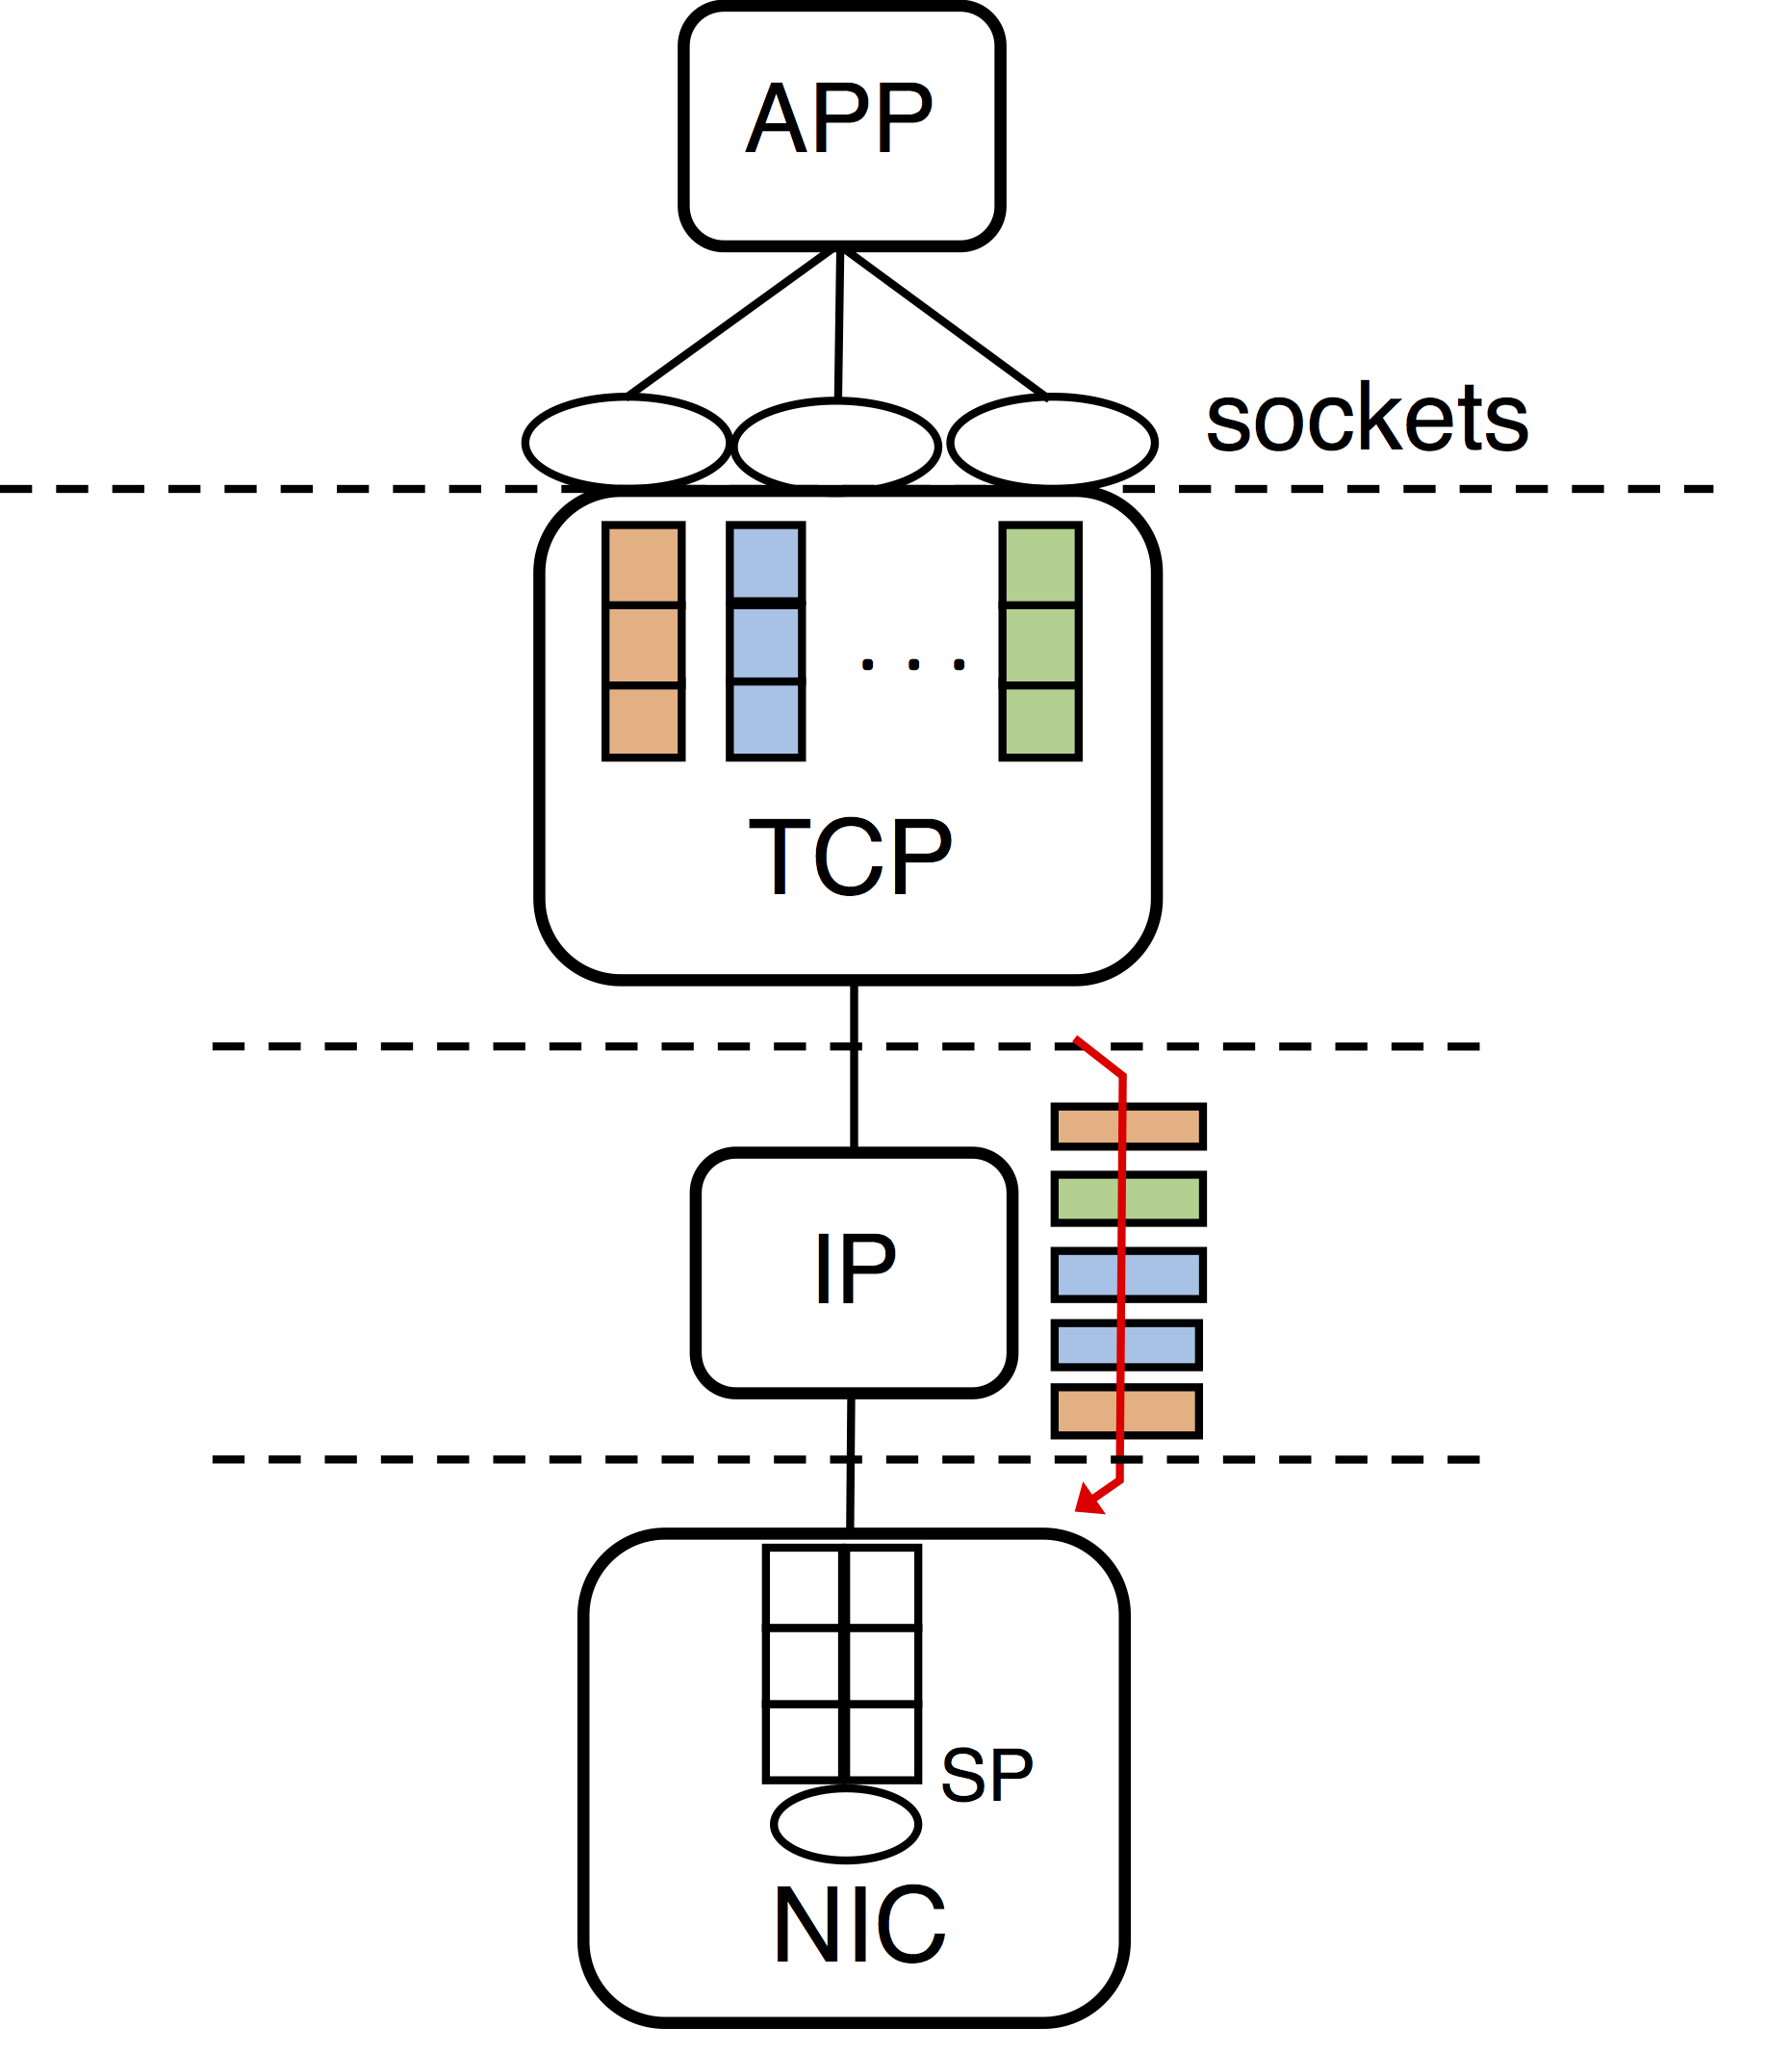
\includegraphics[width=0.4\linewidth]{Chapter4/Figures/tcp-config}
	\caption{Host architecture with TCP. Flows are interleaved thus emulating PS discipline.}
	\label{fig:tcp-config}
\end{figure}%
The architecture of the whole protocol stack at end hosts when adopting TCP is shown in Figure \ref{fig:tcp-config}. First start from the application layer. There is a unique application, following the generation process it setup a new TCP connection for each flow. Hence, already opened TCP sessions are not reused, but they are teared down when the flow completes. For every new connection, the application creates a socket, it batch sends the entire flow through the socket, offloading to TCP the segmentation in packets, then it immediately closes the socket. The application can close immediately the socket because it does not wait any data in response to its flow from the other peer of the TCP connection. There is not interaction, instead it only performs a one-way data transfer. For long flows this approach is not realistic. In a real TCP implementation the operating system would limit the maximum simultaneous bytes it can receive from the user application for preserving the memory allocation in kernel space. However, we can neglect these practical impairments to ease the implementation of the simulator. Opening and closing the socket in this way allows to avoid more complex management of simultaneous connection, like thread creation. Practically, our TCP application has been derived with some changes to the \texttt{TcpSessionApp} class of the standard INET library.\\
From the point of view of TCP, a separated transmission queue is allocated for each new socket. The simulator gave us the possibility to set the queue size limit to infinity. The scheduling among the queues is self-clocked by the TCP ACKs and transmission control mechanisms. A packet is popped from a queue only when the TCP window allow to do so. Simultaneous popping never occurs because ACKs belonging to distinct connections arrive back to back in the worst case. Therefore, packets of different flows are delivered to the IP layer with interleaving. When the socket transmission queue is completely drained, the TCP client immediately send a FIN packet for closing the connection, as the client application has already closed the socket. New connections always run the three-way-handshake during their setup and start with minimum window size. We do not set the initial window increase option of TCP. This is because the bandwidth-delay product of the network amounts to few packets. As a matter of fact, the distances between network elements in data centers are very short and propagation times on the network links are negligible for light speed. For example, on a link of 30m the bit propagation time is roughly 100ns. The transmission time of a TCP ACK packet on a 1Gbps link is 32ns. Thus, differently from large network on geographic scale, the Round Trip Time (RTT) is proportional to the packet transmission times. Since the topology is comprised by very few links, when multiplying the bandwidth and the RTT the result is near 5 packets.
We modified the defualt value of the TCP port range, in order to allow TCP to support the maximum number of simultaneous connection. With the default configuration, new connection could only use ports in the range 32768-61000. We extended the range to 1024-65535. Also, we removed the randomization of the initial sequence number, which is always started from zero. In this way, it is easy to discern the amount of service obtained by a flow and to tag its packets with the right priority. \\
Finally, we tackle at transport layer a possible shortcoming that has been also addressed in PIAS. Since we enforced strict priority queues also in the servers' NICs, that represent the first contention interface for the sender, large backlogs of packets may build up at end hosts. Indeed, the flows demoted to low priority stay active for long and many simultaneous flows share the server access link. They take time to converge to their fair share, meanwhile they increase their window to harvest additional bandwidth. The inet implementation of IP and MAC layer doesn't include back-pressure mechanisms to counteract the aggressiveness of TCP. Thus, either big delays or packet losses may be introduced yet before entering the network. A possible solution is to rate-limit to line rate the data flow between the application and the TCP. However, for the sake of simplicity we acted on the TCP Advertised Window (\texttt{AWND}) to upper bound the sender window to the bandwidth-delay product. Although the effect is practically the same, we are aware that in a real implementation the first solution is more clean. Indeed, the bandwidth-delay product of the topology is in general unknown or not specified to the servers. 
\subsubsection{UDP}
The scenario changes when adopting UDP as a transport protocol. Systems that aim to minimize the Flow Completion Time usually target transport protocols that ensure the delivery of the entire flow, thus neglecting UDP protocol. We tested the system also with UDP essentially for two reasons. First, it is easier to control its behavior, because it do not implement congestion control schemes, retransmissions, timeouts,..It is straightforward to check if the measured load on the topology corresponds to the offered load and verify the correctness of the traffic generation algorithm. Second, it may provide a rude approximation of the FIFO service at flow level, that gave the best results with spatial diversity (\S \ref{sec:dimensioning-spatial}). This is best understood considering Figure \ref{fig:udp-config}. It is well known that differently from TCP, UDP is connectionless. As a consequence, flows are packetized directly at application level and transfered to UDP already broken in datagrams. UDP does not have internal queues nor transmission control schemes, so it forwards all packets to IP, which in turn does the same with the MAC layer, that finally enqueues all packets in the line card buffers. In our simulator this happens in time zero, meaning that all these operations are code routines of the different layers that do not increase the simulation time. In other words, the new flow arrival event at application layer triggers all these network stack operations, which end only once all the packets of the flow are stored in the NIC's buffer. Since the simulator handles one event at a time, nothing else happens in the meantime. The relevant effect is that flows are served fully in FIFO order without interleaving at end hosts. In the network there is statistical multiplexing among different flows, even if the number of concurrent flows in the same interfaces is significantly reduced, due to the discipline enforced at the servers.\\
We use a trivial format for the application message, in order to make few information available on each UDP packet. In particular, we attach to application messages a sequence number and the flow length. Both the information are used for tagging packets with their priorities and to detect at the receiver when the flow is ended.
\begin{figure}[!tb]
	\centering
	\captionsetup{width=.75\linewidth}
	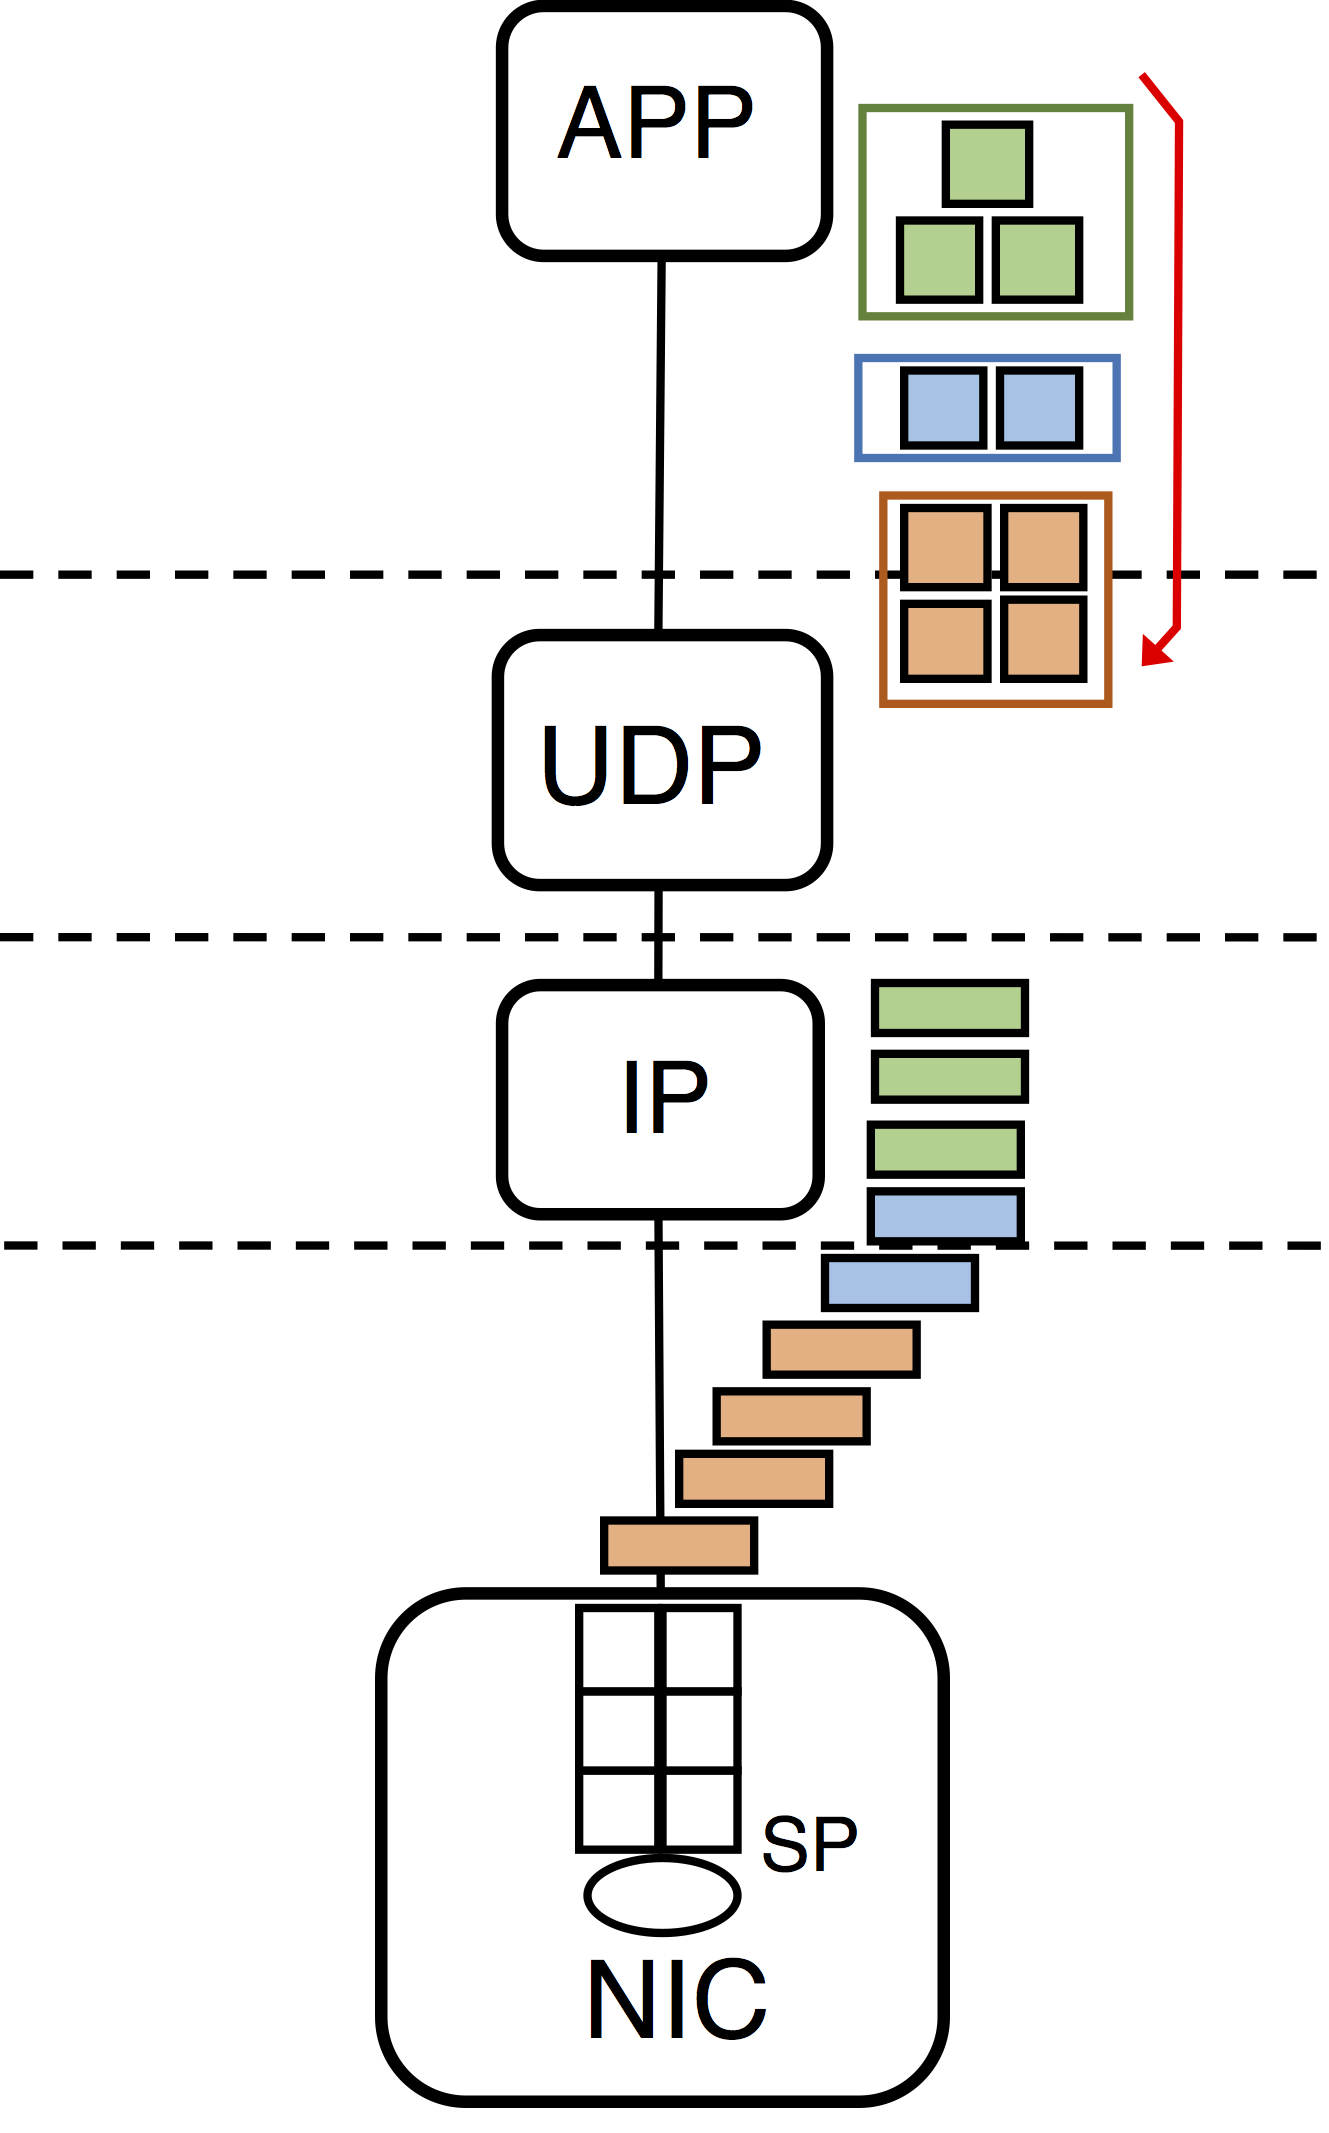
\includegraphics[width=0.3\linewidth]{Chapter4/Figures/udp-config}
	\caption{Host architecture with UDP. Flows are not interleaved thus emulating FIFO discipline.}
	\label{fig:udp-config}
\end{figure}%
\subsection{Network configuration}
% TODO modified djikstra
As discussed in chapter \ref{ch:sdframework}, a radical effect of SD-MLFQ is that the priority of a flow determines its routing over the topology. In a leaf-and-spine network, the ToR switches has to decide in which spine forward every packet, depending on some load balancing criterion. For SD-MLFQ, it is the flow priority, that has been assigned accounting for load balancing. Therefore spatial diversity has to be considered in routing algorithms. \\
We decided to handle the priority-dependent routing with a centralized controller module. End-hosts ask packet-by-packet to the central controller both the priority for their flows and the corresponding route. The controller knows the DC-wide flow size distribution and has computed all the demotion thresholds. Also, it keeps a centralized network view and it knows the priorities configured on every interface in the network. Thus, it can easily respond with a priority code and the route. The route depends on the load balance thresholds and it is provided as a vector of interface identifiers, whereas the priority code depends on the sub-thresholds. End hosts attach the interface IDs to their packets as a control information and tags the packets with the priority code. Finally, they send them through the network. The network devices use the interface identifiers for forwarding packets on the proper links and the priority to enqueue the packets on the proper priority queues. To sum up, it is applied a sort of source routing with the help of a central controller. \\
Both the route requests to the controller and the route information are handled offline, hence they don't contribute as overhead to network traffic. It means they are just data structures and function calls in the simulator. Instead, the priority code is carried in the DSCP field of the IEEE 802.1p \cite{ek1999ieee} standard for VLANs. This was the more immediate and flexible way to have a working prototype, without messing with solutions that make use of standard routing protocols to announce the priorities handled by the network nodes. The actual implementation of spatial diversity routing is out of the scope of this work. We think, however, that a centralized solution would be easy practicable also in modern SDN-based data center networks. \\
%Some changes were required to the inet modules in order to implement spatial diversity mechanism.
At this point, we built the entire topology using only standard inet modules for Ethernet switches with our modification for the forwarding-plane. We configured a single LAN for any topology size and we do not place any IP functionality inside the network. We do not need IP because the routing is handled by the controller. Also, we disabled the computation of the spanning tree and we instructed all servers with predefined entries in the ARP table before the beginning of the simulation. In this way we avoided all the possible problems that might arise from having a unique layer 2 network, such as spanning tree convergence or broadcast storms. Since we do not consider neither network nor server failures, the initial ARP mappings are valid for the entire simulation. We set priorities both at server and switch interfaces to implement the MLFQ scheduler. All priority queues are FIFO queues disciplined by a simple strict priority scheduler. Flow demotion is managed at the sources as explained above. Network switches are left with the only responsibility of choosing the priority queue by reading the DSCP code. \\
All links are Ethernet cables with a length of 30 meters, which seems reasonable in relation to the size of data center buildings. Buffer sizes are set to 1000 packets shared between priority queues of the same interface. Different ports have their own independent memories. We ignored switch architectures with port-shared memory pool, although they are common in data center networks \cite{dctcp, mqecn}.  In the experiments with UDP all queues have unlimited buffer space, in order not to loose packets and allow straightforward FCT measurements at the receiver. This is because packet losses would unnecessarily make controversial the meaning of FCT itself. Despite we are absolutely aware that the system with UDP has no practical value, nevertheless we recognize it has a theoretical utility.
\subsubsection{Priority assignment in down-send}
An aspect that we never addressed in the numerical simulator is how to assign priorities at the egress interfaces, that connect ToR switches to the servers. These ports are last traversed in the \emph{down-send} transmissions before leaving the switching fabric. During the up-send phase of the path from source to destination server we may exploit the spatial diversity to augment the priority classes proportionally to the number of spines. However, when traversing the egress interfaces all the priorities must be in some way mixed and multiplexed to the small number of queues available on a single port. This is illustrated in Fig. \ref{fig:downsend} for the case of rank=4 and two PQs per port, where 8 priorities have to be mapped on two queues. Our observation is that all egress interfaces receive the same DC-wide workload used for generating new flow sizes, because flows are uniformly sent to destination servers. Hence, we treat egress interfaces as in the system without spatial diversity, applying demotion at link level. In our experiments we mostly focused on 2 PQ, thus it was possible to compute rapidly the optimal PIAS threshold.
%\begin{figure}
%	\centering
%	\begin{subfigure}{.45\textwidth}
%		\centering
%		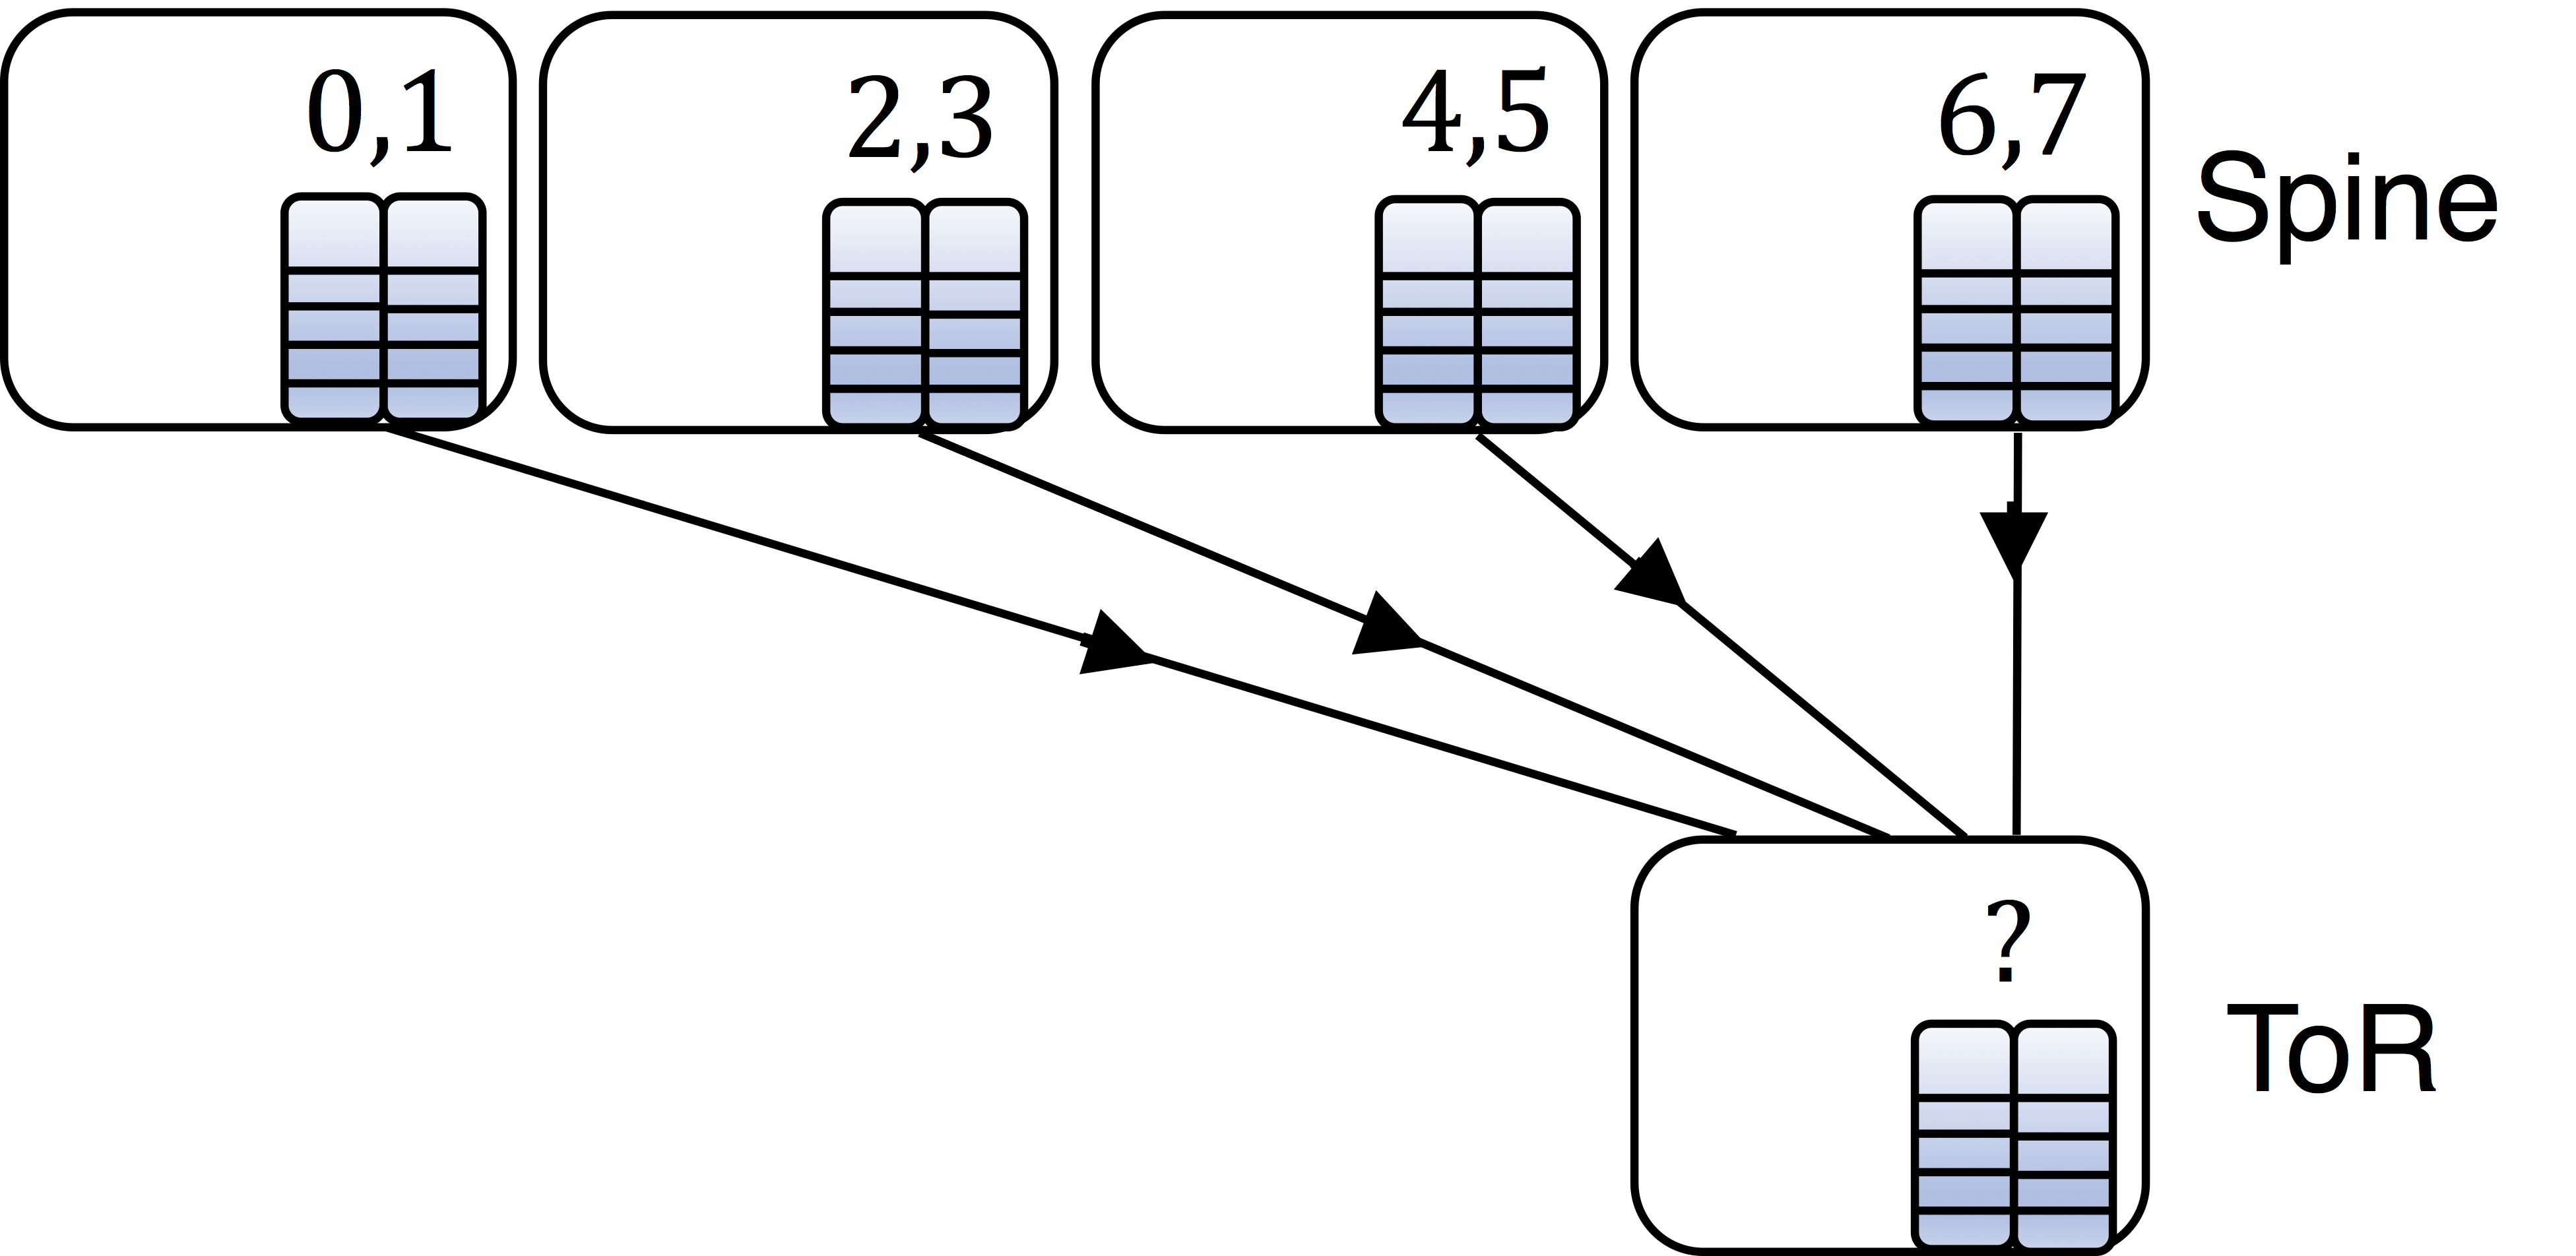
\includegraphics[width=0.99\textwidth]{Chapter4/Figures/downsend}
%		\caption{Example scenario}
%		\label{fig:example-downsend}
%	\end{subfigure}%
%	\hfill
%	\begin{subfigure}{.55\textwidth}
%		\centering
%		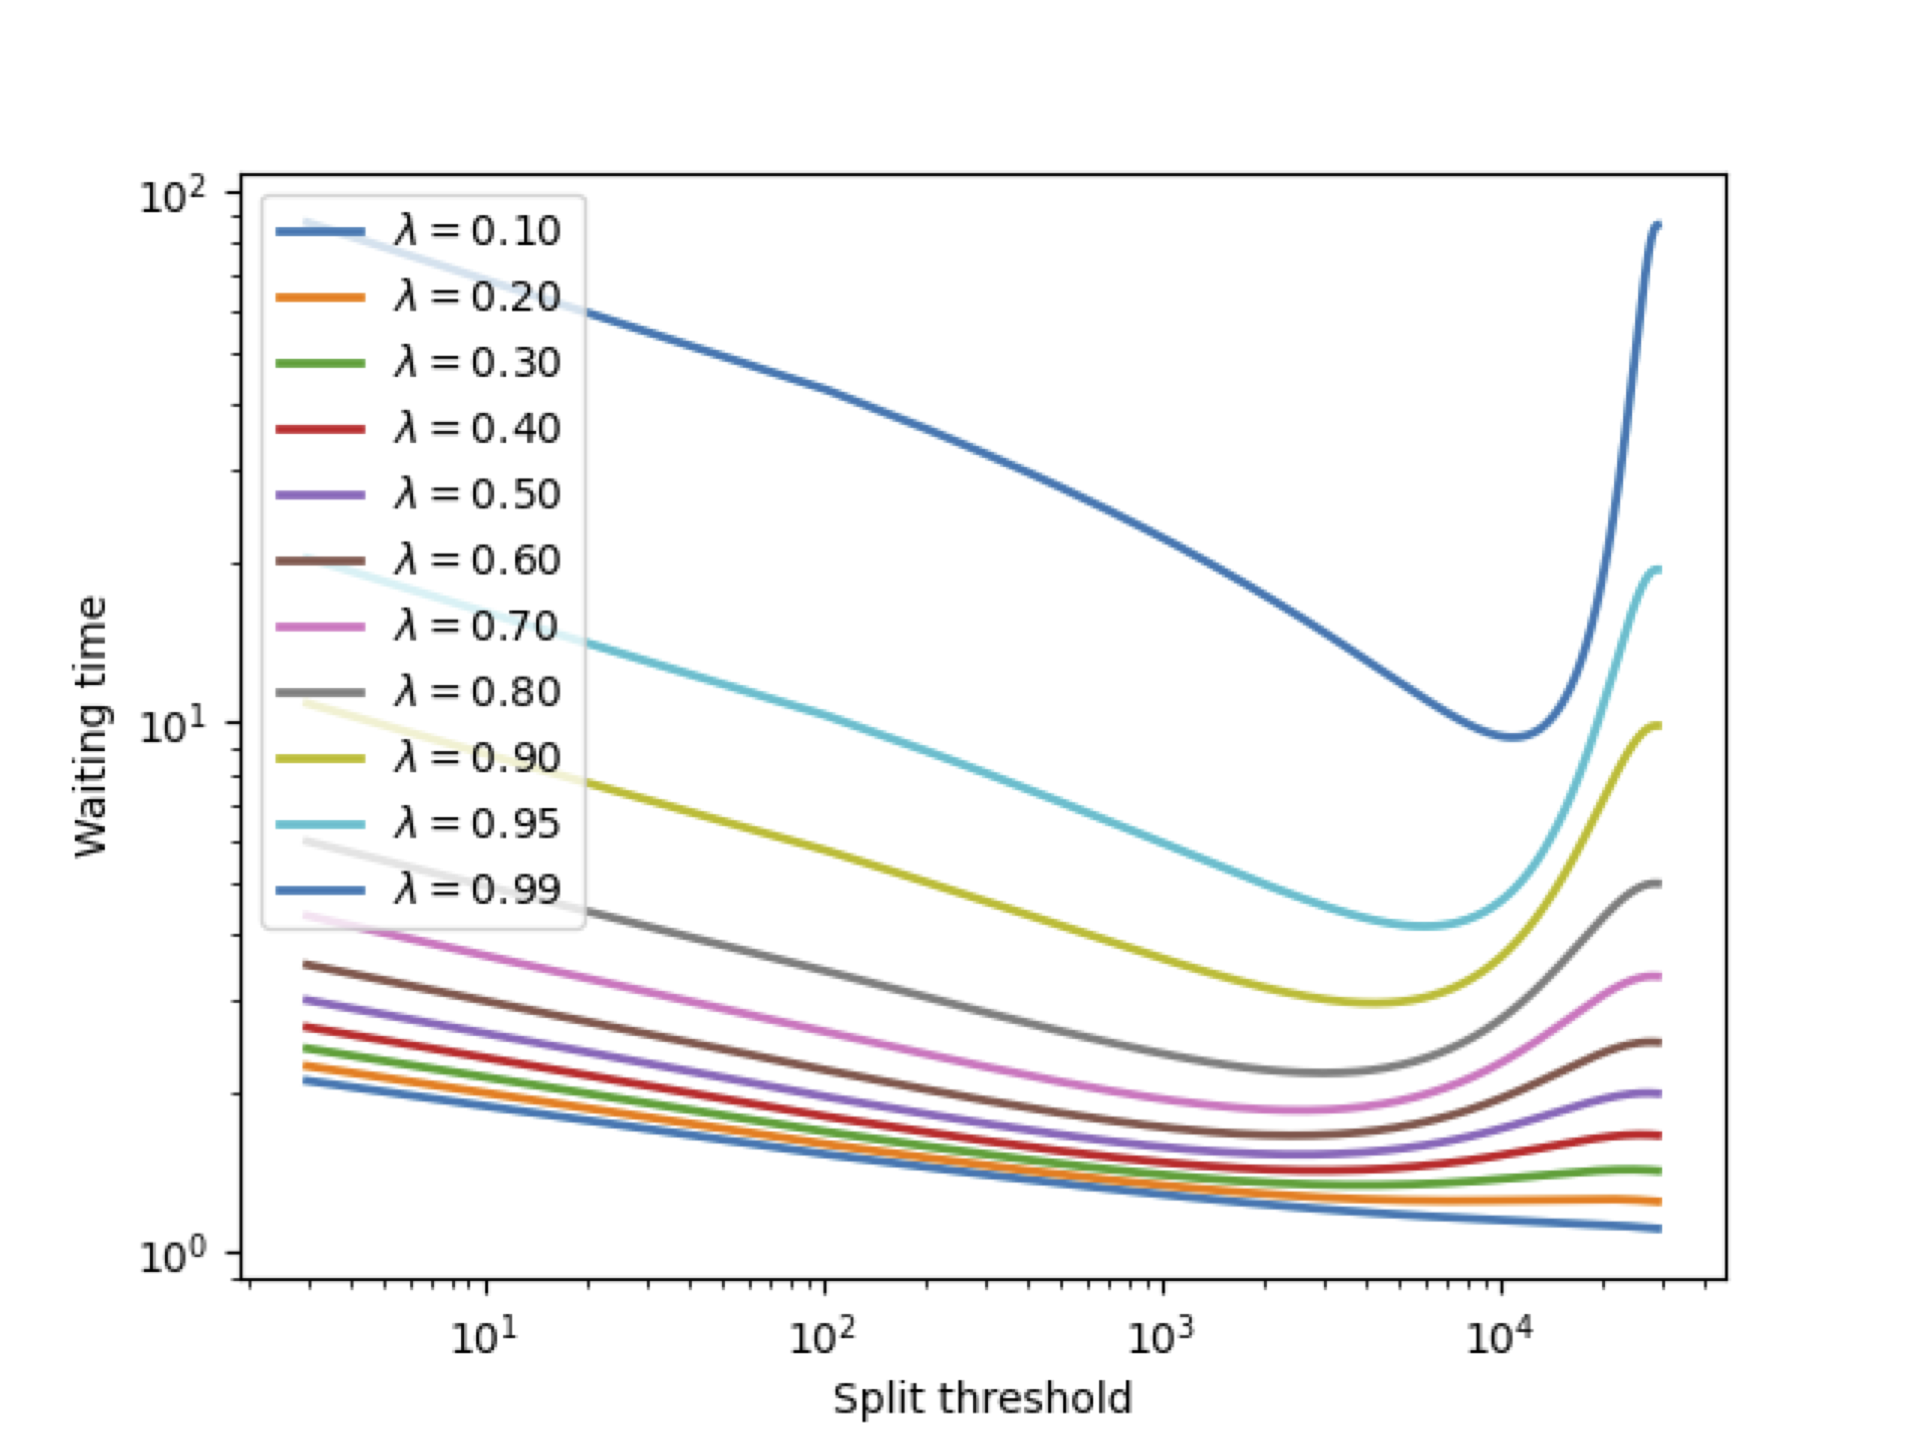
\includegraphics[width=0.99\textwidth]{Chapter4/Figures/opt-2pq}
%		\caption{PIAS thresholds}
%		\label{fig:opt-thresh}
%	\end{subfigure}%
%	\caption{Priority mixture in egress interfaces}
%	\label{fig:downsend}
%\end{figure}
\begin{figure}
	\centering	
	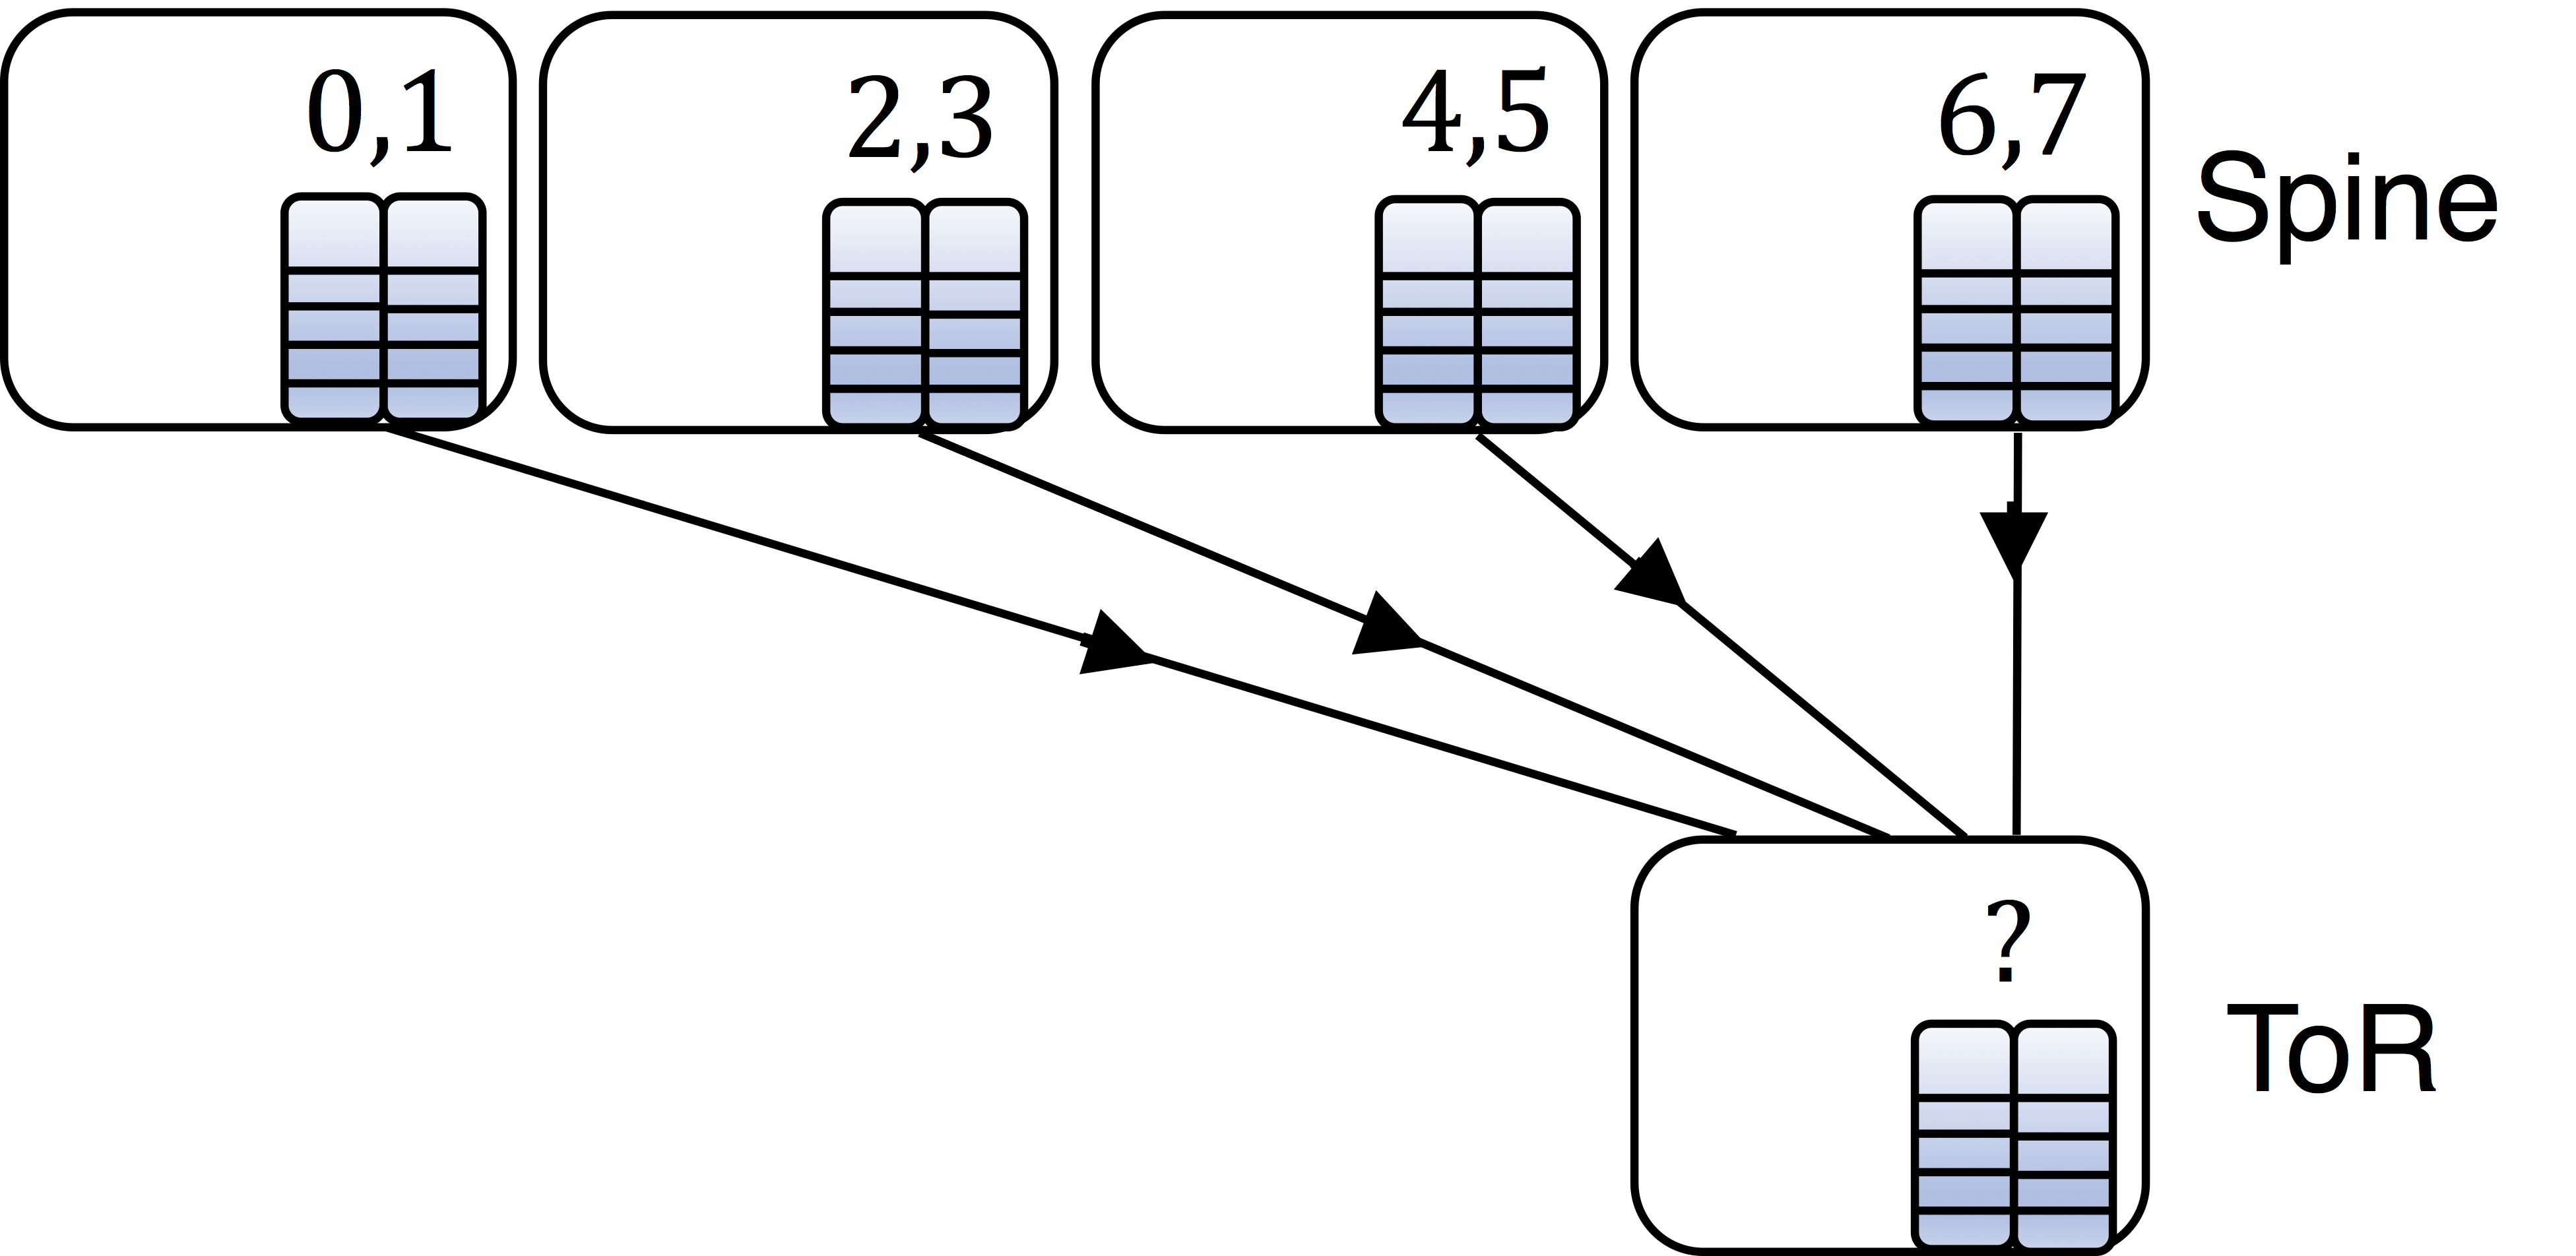
\includegraphics[width=0.5\textwidth]{Chapter4/Figures/downsend}
	\caption{Priority mixture in egress interfaces}
	\label{fig:downsend}
\end{figure}%
\subsection{Datacenter TCP(DCTCP)}
\label{sec:dctcp}
For the final versions of our experiments we employed state-of-the-art DCTCP \cite{dctcp}, among all possible versions of TCP.
Datacenter TCP (DCTCP) is a milestone for transport protocol design in data centers. It actually consists in minimal modifications to TCP New Reno. Its main insight is to leverage Explicit Congestion Notifications (ECN) from the network to properly modulate the window size of the TCP senders. The basic idea behind DCTCP is that queues in the network should be kept as empty as possible to avoid large backlogs that increase latency and do not leave enough headroom to absorb burst arrivals, occurring for example due to incast. Instead of pushing the window to grow until a packet drop is detected, the DCTCP transmitter slows down proactively depending on the level of congestion on the bottleneck link. Network queues mark packets with a congestion signal as soon they exceeds a given occupancy $K$. Then, TCP receivers convey back the congestion signals to TCP transmitters, setting the ECN-Echo bit to 1 in their ACKs. Finally, the TCP sender mantains an estimate $\alpha$ of the fraction of marked packet on an interval of roughly one RTT and modulates the window as:
\[ \text{cwnd} = \text{cwnd} \times (1-\alpha/2)\]
This way, upon mild congestion the window size is gently reduced --- note that only in case $\alpha$=1 it is cut in half as in standard TCP --- still ensuring high throughput, but mitigating its aggressiveness.\\It has been proven that DCTCP effectively succeed in lowering the amplitude of queue oscillations to $O(\sqrt{\text{BDP}})$, instead of $O(\text{BDP})$ of TCP, being BDP the bandwidth-delay product, while not losing throughput for a proper setting of the marking threshold $K$. More importantly, the queue length with DCTCP is proven to be predictable with an analytical expression. In the worst case of $N$ synchronized flows, the queue length is stable around $K+N$. \\
Note that the only requirement from the network is to configure switches with an AQM scheme to mark packets. In practice this can be achieved configuring the RED algorithm, already available in most devices, so that it marks based on the instantaneous queue length and with a unique high and low threshold equal to $K$. 
\subsubsection{DCTCP testbed}
We implemented the above changes to TCP in INET and the ECN markers to plug into the switch interfaces. We deployed the same testbed used in the original article of DCTCP \cite{dctcp}, in order to verify the correctness of the implementation. The testbed topology is shown in \ref{fig:dctcp-testbed-topology}. A group of $N$ server (on the left) start simultaneously long-lived TCP connections towards the same destination server (on the right). We used $N=2$ and $N=20$ and flow sizes fixed to TODO. All links are configured at 1Gbps speed and the DCTCP parameters set according to the guidelines of the reference paper. In particular, the threshold $K$ is set to 20 packets. \texttt{AWND} is set to its maximum value, so that the transmission control is not restricted. Buffer sizes are set to 500 packets.\\ %TODO check\\
\begin{figure}
	\centering
	\begin{subfigure}{.35\textwidth}
		\centering
		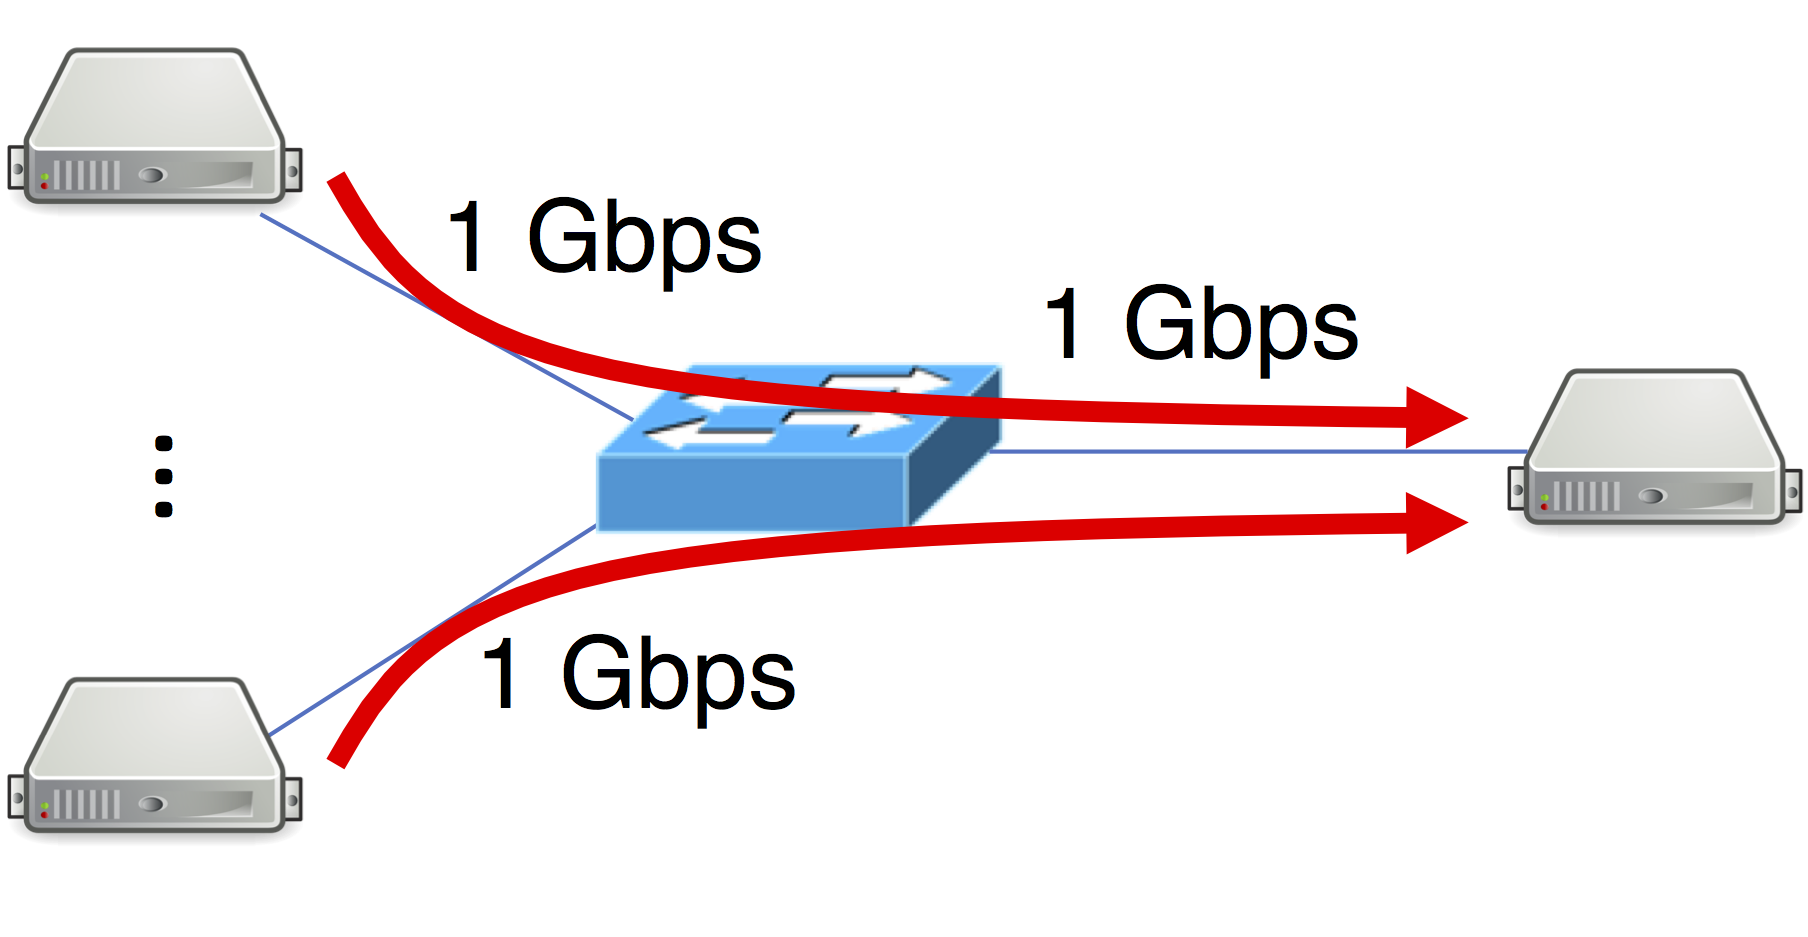
\includegraphics[width=0.99\textwidth]{Chapter4/Figures/dctcp-testbed}
		\caption{Testbed topology}
		\label{fig:dctcp-testbed-topology}		
	\end{subfigure}%
	\hfill
	\begin{subfigure}{.65\textwidth}
		\centering
		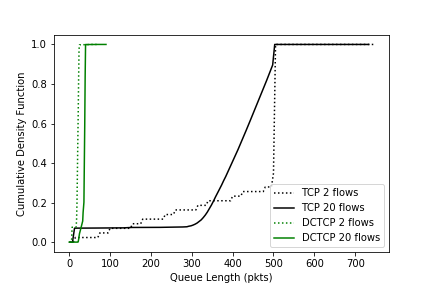
\includegraphics[width=0.9\textwidth]{Chapter4/Figures/dctcp-qlen}
		\caption{CDF of queue length, sampled every 3 packets}
		\label{fig:dctcp-testbed-res}		
	\end{subfigure}%
	\caption{DCTCP implementation testbed}
	\label{fig:dctcp-testbed}
\end{figure}%
We compare the CDF of the queue length when using TCP New Reno and DropTail queues in the bottleneck interface, with the case of DCTCP and ECN-enabled buffers (Fig. \ref{fig:dctcp-testbed-res}).  
It is clearly appreciable the effectiveness of DCTCP, which enforces the queue length to be stable around the predicted value. Conversely, with TCP DropTails the queue variance enlarges significantly, indicating the presence of large oscillations typical of sawtooth pattern induced by TCP AIMD congestion control scheme.
\subsubsection{Integrating ECN with SD-MLFQ}
We set ECN markers only in the network switches with recommended \cite{dctcp} threshold value. Conversely. servers have been equipped with simple DropTail queues and do not adopt AQM schemes. We dealt with few caveats in order to seamlessly integrate ECN rate control with the SD-MLFQ simulator. \\
\textbf{Per-port ECN marking}. First we had to choose how to apply ECN marking to the multi queue scenario. There are fundamentally two choices that trade latency, throughput and fairness. One possibility is to configure the recommended marking threshold independently on each of the $N$ priority queues available. This solution is known as per-queue ECN. It guarantees full link utilization in each priority queue, but the total queue length could potentially grow $N$ times larger and introduce high delays especially to low priority packets. Another option, referred to as per-port ECN, adopts a single marking threshold shared among different priority queues. While ensuring low latency, per-port ECN doesn't provide isolation among queues. Prior work \cite{mqecn} proposed dynamic threshold adjustment to provide best trade-off. We chose to simply use per-port ECN following the same approach as in PIAS. Per-port ECN could help in mitigating the long flow starvation problem. Starvation on low priority queues is undesirable with TCP, since it triggers retransmission timeouts of the connections even if the packets are not lost. Ultimately, it may lead to abrupt connection termination. With per-port ECN and its shared threshold, large buffer pressure on low priority queues helps in slowing down high priority traffic. \\ %TODO verify how many
\textbf{Marking \texttt{SYN/ACK} with CE codepoint.}
According to standardization \cite{ipecn}, ECN capable devices can mark with the congestion signal (\texttt{IP\_CE} - Congestion Experienced codepoint in the IP ToS field) only those packets with the  ECN Capable Transport codepoint set (\texttt{IP\_ECT} codepoint). However, the standard ECN extension to TCP specifies that control packets (\texttt{SYN, ACK, FIN},.) must been transmitted as Non ECN-Capable (\texttt{IP\_NOT\_ECT} codepoint). Thus, if they enter a switch interface when its occupancy exceeds the marking threshold, they are dropped rather than being marked. We noticed in our first simulations with DCTCP an anomalous number of retransmission timeouts (RTOs). We better investigated the number of bytes transmitted when TCP connections experienced RTOs: practically all timeout events occurred at connection setup. Thus, we implemented the modification to TCP that allows ECN-Capable control packets \cite{synecn}.
\section{Result analysis}

%\include{Chapter6/chapter6}
%\include{Chapter7/chapter7}
\bibliographystyle{plain}
\bibliography{biblio}
\paginavuota
\end{document}
